\documentclass[11pt]{article}
\usepackage[T1]{fontenc}
\usepackage{lmodern,microtype}
\usepackage[margin=1in]{geometry}
\usepackage{amsmath,amssymb,amsthm,mathtools}
\usepackage{enumitem,booktabs,longtable,array}
\usepackage{graphicx,xcolor,tikz}
\usetikzlibrary{arrows.meta,calc,positioning,patterns,decorations.pathreplacing}
\usepackage[numbers,sort&compress]{natbib}
\PassOptionsToPackage{hyphens}{url}
\usepackage[colorlinks=true,linkcolor=blue!45!black,citecolor=blue!45!black,urlcolor=blue!45!black]{hyperref}
\numberwithin{equation}{section}
\newtheorem{theorem}{Theorem}[section]
\newtheorem{lemma}[theorem]{Lemma}
\newtheorem{proposition}[theorem]{Proposition}
\newtheorem{corollary}[theorem]{Corollary}
\theoremstyle{definition}
\newtheorem{definition}[theorem]{Definition}
\newtheorem{assumption}[theorem]{Assumption}
\theoremstyle{remark}
\newtheorem{remark}[theorem]{Remark}
\newcommand{\R}{\mathbb R}
\newcommand{\N}{\mathbb N}
\newcommand{\Z}{\mathbb Z}
\newcommand{\eps}{\varepsilon}
\newcommand{\Id}{\operatorname{id}}
\newcommand{\id}{\operatorname{id}}
\newcommand{\cH}{\mathcal H}
\newcommand{\cL}{\mathcal L}
\newcommand{\norm}[1]{\left\lVert #1\right\rVert}
\newcommand{\abs}[1]{\left\lvert #1\right\rvert}
\newcommand{\ind}{\mathbf 1}
\newcommand{\op}{\mathrm{op}}
\DeclareMathOperator{\Lip}{Lip}
\DeclareMathOperator{\supp}{supp}
\DeclareMathOperator{\diam}{diam}
\DeclareMathOperator{\dist}{dist}
\DeclareMathOperator{\rank}{rank}
\DeclareMathOperator{\GL}{GL}
\DeclareMathOperator{\tr}{tr}
\DeclareMathOperator{\conv}{conv}
\DeclareMathOperator{\relint}{relint}
\DeclareMathOperator{\interior}{int}
\DeclareMathOperator{\osc}{osc}
\DeclareMathOperator{\sgn}{sgn}
\setlist{itemsep=3pt,topsep=5pt}
\hypersetup{pdftitle={Strong diffeomorphic approximation in three dimensions for 1 <= p <= 2},pdfauthor={OpenAI}}
\title{Strong diffeomorphic approximation\\in three dimensions for $1\le p\le2$}
\author{OpenAI}
\date{September 24, 2026}
\begin{document}
\maketitle
\begin{abstract}
We resolve the three-dimensional Ball--Evans approximation problem for
$1\le p\le2$. Every $W^{1,p}$ homeomorphism between arbitrary bounded domains
in $\R^3$ is a strong $W^{1,p}$ limit of smooth diffeomorphisms onto the same
target.
\end{abstract}
\section{Introduction and conventions}\label{sec:introduction}

The Ball--Evans approximation problem concerns the compatibility of
Sobolev approximation with global injectivity. A deformation in nonlinear
elasticity is represented by a map between spatial domains; injectivity
expresses noninterpenetration, whereas its weak first derivative records
the local deformation. Smooth approximation is elementary if injectivity
is discarded, but convolution need not preserve it. The question is
whether the two requirements can be met simultaneously. Ball's
formulation explicitly attributes the question to Evans
\cite[Section~3, p.~8]{Ball2001}; his later discussion and Hencl's survey
explain the surrounding variational questions
\cite{Ball2010,Hencl2025}.

Here a \emph{domain} is a nonempty connected open set. For domains
$\Omega,\Lambda\subset\R^3$ and $1\le p<\infty$, a Sobolev
homeomorphism is a homeomorphism $f:\Omega\to\Lambda$ whose components
and weak first derivatives belong to $L^p(\Omega)$. A smooth
diffeomorphism has a smooth inverse as well as a smooth forward map.
The fixed-target version of the approximation problem asks for
diffeomorphisms $f_j:\Omega\to\Lambda$ such that both $f_j-f$ and
$Df_j-Df$ tend to zero in $L^p(\Omega)$. In particular, every
approximating map, not just the limit, must have image exactly
$\Lambda$.

We resolve this problem for the low and critical exponents in dimension
three.

\begin{theorem}\label{main:theorem}
Let $\Omega,\Lambda\subset\R^3$ be nonempty bounded connected open sets, let $1\le p\le2$, and let $f:\Omega\to\Lambda$ be a homeomorphism in $W^{1,p}(\Omega;\R^3)$. There exist $C^\infty$ diffeomorphisms $f_j:\Omega\to\Lambda$, each belonging to $W^{1,p}(\Omega;\R^3)$, such that
\begin{equation}\label{main:convergence}
\int_\Omega\bigl( |f_j-f|^p+|Df_j-Df|^p\bigr)\,dx\longrightarrow0.
\end{equation}
\end{theorem}

Both the map and its inverse in the conclusion are smooth on their open domains. No smoothness at the boundary, boundary extension of $f$, or regularity of either boundary is assumed. Neither inverse Sobolev regularity nor a nonvanishing Jacobian is an additional hypothesis. The target $\Lambda$ is fixed throughout.

\subsection{Prior work and the three-dimensional difficulty}

In the plane, Iwaniec, Kovalev, and Onninen proved strong diffeomorphic
approximation for $1<p<\infty$
\cite[Theorem~1.1]{IwaniecKovalevOnninen2011}. Hencl and Pratelli
established the endpoint $p=1$, including approximation by locally
finite piecewise affine homeomorphisms
\cite[Theorem~1.1]{HenclPratelli2018}. These theorems preserve the
original target and do not require Sobolev regularity of the inverse.
They show that the global topological constraint can be compatible
with strong derivative control throughout the planar exponent range.
The endpoint is a distinct achievement: strict convexity of the
$L^p$ norm is unavailable at $p=1$.

The planar development also distinguishes two mechanisms. The
$p=2$ precursor of Iwaniec, Kovalev, and Onninen used harmonic
replacements and smoothing \cite{IwaniecKovalevOnninen2012}; their
general $p>1$ result used coordinatewise $p$-harmonic replacements.
Hencl and Pratelli's endpoint proof instead used geometric extension
estimates and an adapted grid. Quantitative approximation of
bi-Lipschitz planar maps by Daneri and Pratelli
\cite{DaneriPratelli2014}, and approximation of planar bi-Sobolev
$W^{1,1}$ maps by Pratelli \cite{Pratelli2017}, additionally control
inverse derivatives under their respective stronger hypotheses.
Smooth invertibility of each approximant in Theorem~\ref{main:theorem}
is not a claim of Sobolev convergence of the inverses.

Higher dimensions exhibit a genuine obstruction. Hencl and Vejnar
initiated the counterexamples at $p=1$ \cite{HenclVejnar2016}.
Campbell, Hencl, and Tengvall corrected a gap in that construction and
extended the range to $1\le p<\lfloor n/2\rfloor$ in dimensions
$n\ge4$, with Jacobian determinants of both signs on sets of positive
measure \cite{CampbellHenclTengvall2018}. A sequence of diffeomorphisms cannot
reproduce this sign pattern by strong convergence of its derivatives.
In dimension three, Hencl and Mal\'y's orientation theorem instead
gives $\det Df\ge0$ almost everywhere for a sense-preserving
$W^{1,1}_{\mathrm{loc}}$ homeomorphism
\cite[Theorem~1.1]{HenclMaly2010}. This sign conclusion does not
assert a positive Jacobian and does not furnish an approximation:
rank-deficient derivatives still require separate constructions.

Smoothing a homeomorphism that is already piecewise affine is an
important intermediate problem. Mora-Corral and Pratelli obtained
fixed-image diffeomorphic smoothing in the plane, with control of the
forward map and its inverse \cite{MoraCorralPratelli2014}.
Campbell and Soudsk\'y proved $C^1$ homeomorphic approximation of
piecewise affine maps in arbitrary dimension
\cite{CampbellSoudsky2021}; their conclusion does not require the
inverse to be smooth. Campbell, D'Onofrio, and V\'itek subsequently
proved diffeomorphic smoothing of locally finite piecewise affine
homeomorphisms in dimensions three and four, including forward and
inverse derivative-error control
\cite[Theorem~A]{CampbellDOnofrioVitek2026}. These results identify
the importance of distinguishing a smooth injective map from a
diffeomorphism. They do not construct a strong piecewise affine
approximation of an arbitrary Sobolev homeomorphism.

The present proof separates that approximation problem from smoothing.
It first constructs an onto locally bi-Lipschitz map with small strong
Sobolev error, and then proves a smoothing theorem with arbitrarily
fine pointwise control. Three-dimensional PL topology, developed by
Moise and Bing and used here in Hamilton's relative formulation,
provides qualitative replacements
\cite{Moise1952Approximation,Moise1952Triangulation,Bing1959,Hamilton1976}.
It supplies no derivative estimate. The energy bounds must therefore
come from the parametrizations and measurements used below, rather
than from the mere existence of a topological replacement.

The critical exponent $p=2$ has additional analytic structure.
Cs\"ornyei, Hencl, and Mal\'y proved that a three-dimensional
$W^{1,2}_{\mathrm{loc}}$ homeomorphism has an inverse of locally
bounded variation, and that almost every parallel plane has the
two-dimensional Lusin property
\cite[Theorems~1.1 and~1.3]{CsornyeiHenclMaly2010}. We use these two
statements, respectively, to select reverse rays and to measure
generic image surfaces. Neither is an assumption on the given inverse.
The further analytic ingredients include Whitney's extension theorem
for compatible first jets \cite{Whitney1934} and conformal
parametrization of metric disks \cite{AhlforsBers1960,McMullen2023}.
Their roles and the accompanying local estimates are made explicit
at the point of use.

The complementary range $2<p<\infty$ is treated by a separate
construction in \cite[Theorem~1.1]{OpenAIHigh2026}. The present paper does
not invoke that range theorem or any of its proof modules. The smoothing
theorem proved here holds for all finite exponents; the companion also
includes a complete proof in its Appendix~A.

\subsection{Measurements, local models, and the proof strategy}

The first objective is to replace $f$ by a locally bi-Lipschitz
homeomorphism while estimating derivatives without a quantitative
topological extension theorem. We measure the images of a locally
finite collection of source curves, and also of source surfaces when
$p=2$. A target triangulation gives complementary-dimensional dual
pieces inside its tetrahedra, defined by ties among their largest
barycentric coordinates. Intersections with these pieces determine a
\emph{budget}: each curve
crossing is charged the length of a corresponding target edge, and
each surface crossing is charged the area of a corresponding target
face, with multiplicity. Generic sampling bounds these sums by the
original trace integrals. Local topological changes make the counted
crossings regular; a face-preserving target reparametrization then
concentrates the image length or area near them. Thus
Proposition~\ref{lt:budget-transfer} converts intersection counts into
actual measurements for an onto locally bi-Lipschitz replacement.
All protected local data are retained in buffered regions that are
excluded from the measurements.

Measurements alone give an upper energy bound, not proximity to
$Df$. We therefore retain finitely many disjoint compact sets on
which the values and first derivatives of $f$ are controlled and
the derivative has a fixed positive rank. The discarded derivative
integral is small; rank-zero points carry no such energy. The
construction on these compact sets depends on the rank.
\begin{enumerate}
\item At full rank, compatible first jets extend to local
$C^1$ diffeomorphisms. Radial source changes enlarge an exact germ,
meaning agreement with such a model near the block center, into most
of a small block, so that the map recovers the prescribed
jet there. The surrounding thin region is filled using the trace
budgets. At $p=2$, reverse-ray selection and angular attenuation
control the surface cost of this radial construction
(Lemma~\ref{la:radial-blocks}).
\item At rank one or two, source coordinates split into the
nonzero directions and the kernel of a nearby fixed matrix.
Compressing the kernel reduces the controlled part of a volume block
to a line or plane section. Nearly minimal curve length gives the
correct derivative on a line. At rank two and $p=2$, the sharp
boundary-parametrized disk estimate gives the analogous conclusion
from nearly minimal area (Lemma~\ref{lt:disk}). At rank two and
$p<2$, a further radial construction inside the plane section
provides the needed approximation.
\item Uncontrolled cells are reparametrized relative to their
already chosen boundary values. Below a cell's dimension, radial
collapse bounds its energy by the boundary energy
(Lemma~\ref{lt:collapse}). This fills faces when $p<2$ and volumes
throughout $1\le p\le2$; the critical faces instead use the disk
estimate. The resulting maps preserve the old cell images and
agree on shared faces (Lemma~\ref{la:cell-completion}).
\end{enumerate}

The order of choices is part of the argument. Compact jet bounds and
all finite multiplicative constants are fixed before the excess
neighborhoods and trace errors are made small against them. The
critical radial construction separates the regions whose area can
be suppressed after replacement from those whose area must be measured
in advance; Figure~\ref{la:radial-bands} displays these regions at the
point where their construction is explained. Outside the
retained compact configurations, universal mesh constants multiply
only the small original energy tail. Summable local errors then
yield a global $W^{1,p}$ approximation, not just a locally Sobolev
map. For $p=1$, the line argument uses an elementary squared
length-defect estimate followed by H\"older's inequality, rather
than strict convexity of $L^1$.

Finally, locally bi-Lipschitz maps are approximated strongly by PL
maps using finite local model libraries. Their derivative bounds are
fixed before reducing the exceptional mesh volume. PL smoothing
then uses small edge and vertex neighborhoods with summable costs.
A fine value tolerance makes the smooth map properly homotopic to
the original homeomorphism inside the target; its positive local
degrees and degree one force bijectivity. This proves the fixed
image for each individual approximant, independently of passage
to the limit.

Section~\ref{sec:smoothing} proves this smoothing theorem first.
Section~\ref{sec:low-tools} develops the disk and collapse estimates,
relative topological replacements, and sampled trace budgets.
Section~\ref{sec:low-assembly} constructs the rank-sensitive blocks
and proves their global strong approximation estimate.
Section~\ref{sec:completion} concludes the diffeomorphic
approximation theorem on the original target.

\subsection{Conventions}

Unless stated otherwise, all domains, closures, local finiteness, and compactness are taken relative to the indicated open manifold. A compact set in an open domain has positive distance from its Euclidean complement. A PL map or triangulation is locally finite. A locally bi-Lipschitz homeomorphism has finite Lipschitz constants in both directions on sufficiently small neighborhoods; no global bound is implicit.

The symbol $|A|$ denotes the Frobenius norm of a matrix, and $\|A\|_{\op}$ its operator norm. We use the Frobenius norm in sharp gradient estimates. Equivalent norms give the same strong convergence in Theorem~\ref{main:theorem}. The symbols $\cL^m$ and $\cH^m$ denote Lebesgue and Hausdorff measure. Integrals on parameterized traces include their stated multiplicities. The differential along an $m$-dimensional parameter space is denoted $D_m$ when it must be distinguished from the full differential.

A \emph{fine value tolerance} on a domain $U$ is a positive continuous function on $U$. To approximate finely means to meet a prescribed such tolerance pointwise. Whenever inverse control is needed on a compact localization, it is included in the prescribed tests. Locally finite constructions permit tolerances tending to zero toward the ends of the open domains; no positive global lower bound is assumed.

Constants called \emph{absolute} depend only on dimension and on fixed universal reference shapes. A constant $C_p$ may also depend on the fixed exponent. Other dependencies are specified when the constant is introduced. A finite constant that depends on a chosen compact collection of jets or charts is fixed before an error is required to be small against it.

A homeomorphism between connected oriented domains has a constant topological orientation. If necessary, reflect the target, perform the construction for the orientation-preserving map, and undo the reflection. This convention imposes no extra hypothesis on the Sobolev differential.

\begin{lemma}[Local tolerances]\label{pre:local-tolerances}
Let $U\subset\R^n$ be open and let $a:U\to(0,\infty)$ be continuous. For every $L>0$ there is a positive $L$-Lipschitz function $d$ on $U$ such that
\[
 d(x)\le \min\{a(x),1,L\dist(x,\R^n\setminus U)\}.
\]
There are also positive smooth minorants satisfying prescribed positive continuous upper bounds on their values and first derivatives. One may additionally impose positive constant bounds on a locally finite family of compact regional tests. Finite collections of such requirements can be combined, and error budgets on a countable compact exhaustion can be made summable.
\end{lemma}
\begin{proof}
Extend $e(x)=\min\{a(x),1,L\dist(x,\R^n\setminus U)\}$ by zero outside $U$, and put
\[
 d(x)=\inf_{y\in\R^n}\{e(y)+L|x-y|\}.
\]
This function is $L$-Lipschitz and is bounded above by $e$. It is positive at an interior point $x$: on a small closed ball about $x$, $e$ has a positive minimum, and outside that ball the distance term has a positive lower bound.

For a smooth minorant take a smooth locally finite partition of unity $\{\chi_i\}$ with compact supports in $U$ and put $b=\sum_i c_i\chi_i$, with positive constants $c_i$. Given positive continuous bounds $v,w$, choose
\[
 c_i\le 2^{-i-2}\min\left\{
 \inf_{\supp\chi_i}v,
 \frac{\inf_{\supp\chi_i}w}{1+\|D\chi_i\|_\infty}
 \right\}.
\]
Then $b>0$, $b\le v$, and $|Db|\le w$. Replace a finite list of requirements by their minimum. For countably many regional tests use a locally finite compact cover with compact enlargements, refine the bounds on each intersecting support, and allocate total errors by a convergent positive series. Only finitely many regional requirements meet a given compact support.
\end{proof}

We will also use the following elementary global observation. If $H:U\to V$ is a homeomorphism and a continuous map $G:U\to V$ satisfies
\[
 |G(x)-H(x)|<\tfrac12\dist(H(x),\R^n\setminus V),
\]
then the straight homotopy stays in $V$. When $V$ is bounded, it is a proper homotopy: the preimage of a compact target set is contained, uniformly in the homotopy parameter, in the $H$-preimage of a compact set a positive distance from $\partial V$. This observation will be used together with local injectivity and degree, not as a substitute for local injectivity.

\tableofcontents
\section{Qualitative topology and strong smoothing}
\label{sec:smoothing}

All PL structures in this Section are the ordinary structures on open
subsets of $\R^3$.  Triangulations are locally finite in the open domain.
In particular, neither a triangulation nor the local constants used below
need have uniform behavior at the boundary.

The qualitative PL tools belong to the three-dimensional triangulation
and approximation theory of Moise and Bing
\cite{Moise1952Approximation,Moise1952Triangulation,Bing1959}; Hamilton's
relative formulation \cite{Hamilton1976} is the precise interface used
below. Edwards--Kirby's deformation theorem supplies the supported
ambient extensions \cite{EdwardsKirby1971}. We separate these
topological existence statements from the derivative estimates:
finite local model libraries and subsequently chosen small exceptional
sets provide the latter.

\begin{theorem}[Strong smoothing of locally bi-Lipschitz maps]
\label{sm:smoothing}
Let $\Omega,\Omega'\subset\R^3$ be bounded domains, let
$1\le p<\infty$, and let $H:\Omega\to\Omega'$ be a locally
bi-Lipschitz homeomorphism in $W^{1,p}(\Omega;\R^3)$.  For every
$\eps>0$ and every continuous function $\xi:\Omega\to(0,\infty)$,
there is a $C^\infty$ diffeomorphism $g:\Omega\to\Omega'$ such that
\begin{equation}
 \label{sm:smoothing-conclusion}
 \norm{g-H}_{W^{1,p}(\Omega)}<\eps,
 \qquad |g(x)-H(x)|<\xi(x)\quad(x\in\Omega).
\end{equation}
In particular, $g$ belongs to $W^{1,p}(\Omega;\R^3)$, and the
approximations have exactly the target $\Omega'$.
\end{theorem}

The proof has two parts.  First we smooth a locally finite PL
homeomorphism with summable local derivative errors.  We then approximate
$H$ by such a PL map.  In the second part a finite collection of local
models gives derivative bounds before the measure of the exceptional
mesh cubes is made small.  The qualitative topology used to choose those
models supplies no derivative estimate.

\subsection{Relative qualitative tools}

\begin{lemma}[Fine relative PL approximation]
\label{sm:relative-pl}
Let $M,N$ be PL three-manifolds without boundary, with $N$ metrized,
and let $f:M\to N$ be a homeomorphism.  Suppose that $K\subset M$ is
closed and that $f$ is PL on an open neighborhood of $K$.  Given a
continuous function $\eta:M\to(0,\infty)$, there is a PL
homeomorphism $f_1:M\to N$ which agrees with $f$ on a neighborhood of
$K$ and satisfies
\[
 d_N(f_1(x),f(x))<\eta(x)\qquad(x\in M).
\]
Noncompact manifolds are allowed.  For manifolds with boundary the same
statement holds if $K$ contains $\partial M$ and $f$ is PL near $K$.
\end{lemma}

\begin{proof}
Choose a closed neighborhood $K^+$ of $K$ contained in the open set on
which $f$ is PL.  Transport the PL structure of $N$ to $M$ by $f$.
The identity from the original structure to the transported structure
is PL near $K^+$.  Hamilton's relative approximation Theorem
\cite[Section~3, Theorem~2.2, pp.~68--69]{Hamilton1976} applies to these
two structures.  Use the compatible metric
$d_f(x,y)=d_N(f(x),f(y))$ and the fine tolerance $\eta$.
It gives a homeomorphism $a$ that is PL between the two structures,
is the identity on $K^+$, and satisfies
$d_f(a(x),x)<\eta(x)$.  Then $f_1=f\circ a$ has all the asserted
properties.  The boundary condition in Hamilton's Theorem is precisely
the additional condition stated here; for an open Euclidean domain its
manifold boundary is empty.
\end{proof}

\begin{lemma}[Small local ambient extension]
\label{sm:local-extension}
Fix a closed Euclidean cube $B\subset\R^3$, compact sets $C,D\subset B$
with $C\subset\operatorname{int}B$, and an open neighborhood $O$ of
$C\cup D\cup\partial B$.  For every $\lambda>0$ there is a
$\delta>0$, depending only on these source sets and on $\lambda$,
with the following property.  If $e:O\to\R^3$ is an embedding,
\[
 \sup_{x\in O}|e(x)-x|<\delta,
 \qquad e=\Id\ \hbox{on }D\cup\partial B,
\]
then there is a homeomorphism $A:\R^3\to\R^3$ such that
\begin{equation}
 \label{sm:extension-conclusion}
 A=e\ \hbox{on }C,\qquad
 A=\Id\ \hbox{on }D\cup(\R^3\setminus\operatorname{int}B),
 \qquad \sup_{\R^3}|A-\Id|<\lambda.
\end{equation}
The number $\delta$ is uniform over a finite list of fixed normalized
configurations $(B,C,D,O)$.  No derivative bound on $e$ is required.
\end{lemma}

\begin{proof}
Put $E=C\cup D\cup\partial B$.  The deformation Theorem of
Edwards--Kirby \cite[Theorem~5.1]{EdwardsKirby1971}, applied at the
inclusion of $O$ in $\R^3$, deforms every sufficiently close embedding
$e$ through embeddings $e_t$, starting at $e_0=e$, so that
$e_1=\Id$ on $E$.  The deformation is unchanged outside a fixed
compact neighborhood $L$ of $E$ in $O$, and fixes the inclusion.
Its continuity at the inclusion permits us to require
\[
 |e_t(x)-x|<\lambda/2\quad(x\in L,\ 0\le t\le1),
 \qquad |e(x)-x|<\lambda/2\quad(x\in L).
\]
A sufficiently small uniform $\delta$ on $O$ meets the finitely many
compact-open conditions that specify this neighborhood of the
inclusion.  In the terminology of that Theorem a proper embedding
respects manifold boundaries; this condition is automatic for the
ambient manifold $\R^3$.

All the open images $e_t(O)$ coincide.  To see this, enclose $L$ in a
finite union of relatively compact subdomains of $O$ whose boundary collars are outside
the region where the deformation changes the map.  The embeddings
agree on that collar. Invariance of domain
\cite[Theorem~2B.3]{Hatcher2002} and degree relative to
the common boundary show that the images of the enclosed subdomain
are the same.  Outside it the maps already agree.
On this common open image define
\[
 A_0=e\circ e_1^{-1},
\]
and define $A_0$ to be the identity elsewhere.  The map is already
the identity off the compact set $e_1(L)$ in the common image, so
this is an ambient homeomorphism.  It agrees with $e$ on $E$ and has
displacement less than $\lambda$.  Since it fixes $\partial B$
pointwise, it preserves the bounded complementary component
$\operatorname{int}B$.  Restrict $A_0$ to $B$ and extend it by the
identity outside $B$ to obtain $A$.

The construction uses only the displayed source configuration and
continuity at the inclusion.  For finitely many normalized
configurations take the minimum of the resulting positive tolerances.
\end{proof}

We will use Lemma~\ref{sm:local-extension} when the input embedding is
defined by a small map $\eta$ near a new core and by the identity near
older protected sets.  The following observation specifies the required
gluing condition.  Choose open sets
$\overline{O_0}\subset U_0$, where $\eta$ is defined on $U_0$, and
an open set $V$ containing the protected sets, such that
$\eta=\Id$ on $U_0\cap V$.  If $\eta$ is sufficiently close to
the identity that $\eta(O_0)\subset U_0$, the map
\begin{equation}
 \label{sm:patched-embedding}
 e=\eta\ \hbox{on }O_0,\qquad e=\Id\ \hbox{on }V
\end{equation}
is an embedding.  Indeed, a collision $\eta(x)=y$ with
$x\in O_0$ and $y\in V$ has $y\in U_0\cap V$, whence
$\eta(y)=y$ and injectivity of $\eta$ gives $x=y$.  The open
embedding property then follows from invariance of domain.  All the
sets in this observation can be fixed in advance when the source
configurations range over a finite list.

\begin{lemma}[Fine control, properness, and the target]
\label{sm:proper-degree}
Let $h:\Omega\to\Omega'$ be an orientation-preserving homeomorphism
between bounded domains, and let $g:\Omega\to\R^3$ be a smooth
map with $\det Dg>0$.  If
\begin{equation}
 \label{sm:target-distance}
 |g(x)-h(x)|<\frac12\dist(h(x),\R^3\setminus\Omega')
 \qquad(x\in\Omega),
\end{equation}
then $g$ is a diffeomorphism of $\Omega$ onto $\Omega'$.
\end{lemma}

\begin{proof}
Write $d(y)=\dist(y,\R^3\setminus\Omega')$ and
$g_t=(1-t)h+tg$.  Condition~\eqref{sm:target-distance} puts the entire
segment $g_t(x)$ in $\Omega'$.  Since $d$ is 1-Lipschitz,
\[
 d(g_t(x))\le\frac32d(h(x)).
\]
If $K\Subset\Omega'$ and $m=\min_Kd>0$, the inverse image of $K$
under the homotopy lies in
\[
 h^{-1}\bigl(\{y\in\Omega':d(y)\ge2m/3\}\bigr)\times[0,1].
\]
The set in braces is compact because $\Omega'$ is bounded.
Thus $g_t$ is a proper homotopy.  Its endpoint $g$ has the same
degree as $h$, namely one.  A proper local diffeomorphism has
finitely many preimages of each point, and here each preimage has
positive local degree.  The degree-one identity therefore says that
every point of $\Omega'$ has exactly one preimage.  The local smooth
inverses patch to a smooth inverse on $\Omega'$.
\end{proof}

\subsection{Smoothing a locally finite PL homeomorphism}

\begin{proposition}[Strong PL smoothing]
\label{sm:pl-smoothing}
The conclusion of Theorem~\ref{sm:smoothing} holds if $H$ is replaced
by a locally finite PL homeomorphism
$h:\Omega\to\Omega'$ in $W^{1,p}(\Omega;\R^3)$.
\end{proposition}

\begin{proof}
An orientation-reversing Euclidean isometry in the target reduces
the proof to the orientation-preserving case.  Fix a locally finite
affine triangulation for $h$.  We prescribe summable error budgets
for its edges, vertices, and a locally finite family of compact sets
covering the remainder of the domain.  All modifications below can
also obey an arbitrary positive continuous value tolerance.

\paragraph{The open edges.}
Around each open edge choose a tube of radius $d(t)$, where
$0<t<l$ is its axial coordinate.  The tubes of distinct open edges
are disjoint, their radii are bounded by a small multiple of
$\min(t,l-t)$, and $d$ is exactly linear near both endpoints.
These choices follow from the finite geometry of each simplex star;
local finiteness makes them compatible throughout $\Omega$.
We may make $\norm{d'}_\infty$ small by decreasing the width.

In positively oriented orthogonal frames, and after translations,
the original map on this tube is
\begin{equation}
 \label{sm:edge-form}
 (t,r,\theta)\longmapsto
 \bigl(at+r b(\theta),\;r s(\theta)e_{\phi(\theta)}\bigr),
 \qquad e_\alpha=(\cos\alpha,\sin\alpha),
\end{equation}
where $a>0$, $s>0$, and the coefficients are smooth on the closed
angular sectors.  The transverse homogeneous map is injective:
otherwise two equal transverse images, taken at arbitrarily small
radius, would have their axial difference canceled by changing $t$,
contradicting injectivity of $h$ in the edge star.  Its angular
map is consequently an orientation-preserving circle
homeomorphism.  We choose a lift $\phi$ with
$\phi(\theta+2\pi)=\phi(\theta)+2\pi$.
Positive determinants on the finitely many sectors give upper and
positive lower bounds for $s$ and for the one-sided derivatives
$\phi'$.

Choose constants $c>0$ and $c'$, and for $0\le\tau\le1$ put
\[
 b_\tau=(1-\tau)b,\qquad
 s_\tau=(1-\tau)s+\tau c,\qquad
 \phi_\tau=(1-\tau)\phi+\tau(\theta+c').
\]
For fixed $\tau$, the determinant of the corresponding map in the
frame $(\partial_t,\partial_r,r^{-1}\partial_\theta)$ is
\begin{equation}
 \label{sm:edge-determinant}
 a s_\tau^2\phi_\tau'>0.
\end{equation}
On all the closed sectors and all $\tau\in[0,1]$ this has a
positive minimum.  Let $\chi$ be a smooth cutoff equal to 1 on
$(-\infty,-1]$ and to 0 on $[-1/2,\infty)$, and substitute
\[
 \tau(t,r)=\chi\!\left(\frac{\log(r/d(t))}{N}\right)
\]
in the preceding formula.  The additional derivative columns have
size at most
\begin{equation}
 \label{sm:edge-cutoff-error}
 \frac{C}{N}\bigl(1+\norm{d'}_\infty\bigr).
\end{equation}
Indeed, $|r\partial_r\tau|\le C/N$ and
$|r\partial_t\tau|\le C(r/d)|d'|/N$, while $r/d\le1$ on
the support of the modification.  The remaining factors come from
the fixed angular data.  Taking $N$ large preserves positive
determinants on every sector, including one-sided limits.
Near the axis the result is the nonsingular affine map
$(t,r,\theta)\mapsto(at,cr e_{\theta+c'})$.
Near the tube boundary it agrees with $h$.

All first derivatives are bounded by an edge-dependent constant
independent of a further common decrease of $d$.  The volume of the
tube tends to zero under that decrease.  Both its derivative error
and its value error therefore have arbitrarily small $W^{1,p}$
cost.  Choose these costs summably over the edges and call the
result $h_1$.  It is continuous and locally Lipschitz, fixes all
vertices, and has the required small total error.  Because the
tube widths are exactly linear near endpoints, $h_1-h_1(v)$ is
homogeneous of degree one on a sufficiently small ball about every
vertex $v$.

\paragraph{The faces and the punctured vertex balls.}
Away from the vertices, the closed convex hull of the nearby
almost-everywhere gradients of $h_1$ is contained in
$\GL^+(3)$ on a sufficiently small neighborhood of each point.
At a smooth point this follows by continuity.  At a nonsmooth
point the only remaining interface is one face.  If $A_-$ and
$A_+$ are its two gradient traces, continuity gives agreement on
the tangent plane, so $A_+-A_-$ has rank at most one with normal
covector to that face.  Consequently
\begin{equation}
 \label{sm:face-segment}
 \det\bigl((1-t)A_-+tA_+\bigr)
 =(1-t)\det A_-+t\det A_+>0\quad(0\le t\le1).
\end{equation}
The traces vary continuously on the two sides.  Their nearby
convex hull lies in a sufficiently small neighborhood of this
compact positive-determinant segment, proving the assertion.
Homogeneity makes this property uniform at relative scale on
a punctured ball about a vertex: cover the unit sphere by finitely
many of the corresponding neighborhoods and rescale.

Let $\rho\ge0$ be a smooth probability kernel supported in the
unit ball.  Away from vertices define
\begin{equation}
 \label{sm:variable-convolution}
 h_2(x)=\int_{\R^3}h_1(x+w(x)z)\rho(z)\,dz,
\end{equation}
where $w$ is smooth and positive there and the integration balls
lie in $\Omega$.  Its derivative is
\begin{equation}
 \label{sm:variable-convolution-derivative}
 Dh_2(x)=\int Dh_1(x+w(x)z)\rho(z)\,dz
 +\int \bigl(Dh_1(x+w(x)z)z\bigr)\otimes Dw(x)\rho(z)\,dz.
\end{equation}
The first integral is in the positive-determinant convex hull just
described.  Taking $w$ and $|Dw|$ sufficiently small locally makes
the second integral a small perturbation, and hence gives
$\det Dh_2>0$.  Formula~\eqref{sm:variable-convolution} is smooth
where $w>0$, as is also seen by writing its smooth variable kernel
in the integration variable $y=x+w(x)z$.

On a small punctured ball at $v$ choose
$w(x)=c_v|x-v|$, with $c_v>0$ sufficiently small.  This is
consistent with the relative-scale convex-hull condition and
makes $h_2-h_1(v)$ homogeneous on a smaller ball.  Set
$h_2(v)=h_1(v)$ there.  The required radius function exists by
a locally finite partition of unity with sufficiently small
positive coefficients.  Near the vertices blend this function
with $c_v|x-v|$ on disjoint annuli.  The annular cutoff terms
are bounded by a constant times $c_v$ if the competing radii
are chosen at that same small scale, so both the radius and
gradient restrictions survive.  This is also an instance of
the local minorant construction in Lemma~\ref{pre:local-tolerances}.

Here is the global error choice.  First take disjoint vertex balls
so small that their volumes, multiplied by the fixed local
gradient bounds to the power $p$, meet a summable error budget.
On these balls the gradients in
Equation~\eqref{sm:variable-convolution-derivative} are bounded independently
of a further decrease of their radii.  On a compact set outside
the balls, the local gradients are bounded and converge at every
piecewise smooth point as $w,|Dw|\to0$.  Dominated convergence
therefore gives an arbitrarily small derivative error on that
compact set.  A locally finite compact covering with summable
budgets makes the total $W^{1,p}$ error as small as prescribed.
The value error follows from local Lipschitz continuity and the
small radius.  These arguments include $p=1$.

\paragraph{The vertices.}
Center a homogeneous vertex ball at the origin and subtract
$h_1(v)$.  Write the resulting map as $F$.  Euler's identity is
$DF(x)x=F(x)$.  Since $DF(x)$ is invertible for $x\ne0$, $F(x)$
never vanishes there.  We can thus write
\begin{equation}
 \label{sm:vertex-form}
 F(r\theta)=rR(\theta)\Phi(\theta),\qquad
 R>0,\quad\theta\in S^2.
\end{equation}
Its positive determinant implies that $\Phi:S^2\to S^2$ is a
smooth orientation-preserving local diffeomorphism.  It is a
covering by compactness, and it is one-sheeted because $S^2$ is
simply connected.

Smale's Theorem gives a smooth isotopy $\Phi_\tau$ from $\Phi$
to a rotation, smooth jointly in $(\tau,\theta)$
\cite[Theorem~6]{Smale1959}; for the jointly smooth deformation see also
\cite[Theorem~1.5]{LiWatts2011}.  Interpolate $R$ through positive
functions $R_\tau$ to a positive constant.  For fixed $\tau$ the
homogeneous map
$F_\tau(r\theta)=rR_\tau(\theta)\Phi_\tau(\theta)$
has determinant
\[
 R_\tau(\theta)^3 J_{S^2}\Phi_\tau(\theta)>0.
\]
The family has bounded first derivatives and a positive
determinant minimum, by compactness.  On an arbitrarily small
ball replace $F$ by $F_{\tau(r)}$, where $\tau$ is 0 near the
outer boundary, 1 near the center, and
$\sup_r|r\tau'(r)|$ is sufficiently small.  Such a transition
is obtained by spreading a fixed cutoff over a sufficiently
long interval of $\log r$.  Its extra derivative term is
bounded by $C|r\tau'(r)|$, so positive determinant persists.
At the center the map is a dilation followed by a rotation.
It is therefore smooth and nonsingular there.

The derivative bound for this last modification depends on the
fixed spherical isotopy but not on the support radius.  Shrinking
that radius gives arbitrarily small summable $W^{1,p}$ costs
over all vertices.  The resulting map $g$ is smooth and has
positive determinant throughout $\Omega$.

Finally, in each of the three operations impose local value
tolerances whose sum is less than
\[
 \min\!\left\{\xi(x),\frac12
 \dist(h(x),\R^3\setminus\Omega')\right\}.
\]
The preceding constructions permit these fine tolerances and a
total Sobolev error less than $\eps$.  Lemma~\ref{sm:proper-degree}
makes $g$ a diffeomorphism onto the original target.  This proves
the Proposition.
\end{proof}

\begin{remark}
Theorem~A of Campbell--D'Onofrio--V\'itek
\cite{CampbellDOnofrioVitek2026} also gives diffeomorphic
approximation of locally finite piecewise affine homeomorphisms
in dimension three.  Proposition~\ref{sm:pl-smoothing} records the
specific local and fine-control construction needed here; the
reduction from a general locally bi-Lipschitz map is proved next.
\end{remark}

\subsection{Fine meshes and controlled patch insertion}

It remains to approximate $H$ strongly by a PL homeomorphism.
Near most points, an affine first-order model will control the new
derivative. On the remaining patches, qualitative topology provides
replacements but gives no bound for their slopes. Choosing those
replacements only after making the exceptional patches small would
therefore leave the energy estimate circular. We instead select finite
libraries of replacements on each coarse neighborhood, fixing their
derivative bounds before the final mesh resolution. The mesh and
insertion lemmas below let neighboring replacements retain exactly
the same data on their overlaps.

Fix a coarse, locally finite Whitney decomposition $\mathcal P$ of
$\Omega$ into closed dyadic cubes with disjoint interiors.  Choose
relatively compact enlarged neighborhoods $U_P$ that are still locally
finite.  Enlarge them a fixed finite number of times when necessary.
Since $H$ is locally bi-Lipschitz, there are constants $K_P\ge1$ such
that
\begin{equation}
 \label{sm:coarse-bilip}
 K_P^{-1}|x-y|\le |H(x)-H(y)|\le K_P|x-y|
 \qquad(x,y\in U_P).
\end{equation}
Enlarge $K_P$ also to bound $|DH|$ almost everywhere on $U_P$ in the
chosen matrix norm.  The constants may incorporate the data from finitely many neighboring
coarse cubes.  All references below to data local to $P$ allow this
finite enlargement, but never an enlargement depending on the final
fine-mesh resolution.

\begin{lemma}[Adapted dyadic meshes]
\label{sm:mesh}
There is an absolute integer $n_0$ with the following property.
Given arbitrary positive local upper bounds on the fine scale, there
is a locally finite dyadic cube decomposition $\mathcal Q$ of $\Omega$
with centers $c_Q$ and side lengths $l_Q$ for which, on writing
\begin{equation}
 \label{sm:patch-box}
 B_Q(s)=c_Q+[-s l_Q,s l_Q]^3,
\end{equation}
the following hold:
\begin{enumerate}[label=\textup{(\roman*)}]
 \item $B_Q(100)\Subset\Omega$, and cubes meeting $B_Q(50)$ have
 side lengths comparable to $l_Q$ by absolute constants.
 \item The normalized cube configurations in $B_Q(6)$ belong to a
 finite list.  There is a conforming affine triangulation of
 $\mathcal Q$ with finitely many normalized nondegenerate shapes
 on these configurations.
 \item The cubes have $n_0$ colors so that the closed boxes $B_Q(6)$
 of a single color are pairwise disjoint.
 \item Attach to $Q$ a coarse index $P(Q)$ containing $c_Q$, using
 a fixed convention on coarse boundaries.  The initial scale
 bounds can be reduced so that all interactions through any fixed
 number of neighboring patch layers are confined to a fixed
 locally finite graph of coarse indices, independent of further
 mesh refinement.  The corresponding patches lie in the
 neighborhoods on which the required bounds in
 Equation~\eqref{sm:coarse-bilip} hold.
\end{enumerate}
The upper bounds on the fine scale remain arbitrarily prescribable.
\end{lemma}

\begin{proof}
Choose a positive size function $s$ on $\Omega$ with sufficiently
small absolute Lipschitz constant, below all the prescribed local
bounds and below $10^{-3}\dist(x,\R^3\setminus\Omega)$.
Lemma~\ref{pre:local-tolerances} supplies such a minorant.  Take the
maximal dyadic cubes for which
\[
 l_Q\le\inf_Qs.
\]
Failure of the condition for the dyadic parent gives
$s(x)\le(2+C\Lip(s))l_Q$ on $Q$.  The small Lipschitz constant
then gives local comparability on $B_Q(50)$.  For example, choosing
it sufficiently small makes every dyadic ratio in this neighborhood
belong to $\{1/2,1,2\}$.  The distance bound puts $B_Q(100)$ inside
$\Omega$.  Maximality gives a decomposition, and the positive lower
bound for $s$ near every compact subset gives local finiteness.

The cube vertices have dyadic coordinates.  Bounded local scale
ratios and bounded normalized distance therefore give only finitely
many normalized configurations.  To triangulate, decompose each
cube face into its square contact facets with adjacent cubes.
Put every contact vertex and hanging subdivision point on the
perimeter of each such square.  Cone these perimeter segments from
the square center, and then cone the resulting triangulation of
each cube boundary from the cube center.  The constructions on
shared facets agree.  They give nondegenerate simplices, and their
normalized shapes range over a finite list.

Local comparability bounds the degree of the graph joining cubes
whose $B_Q(6)$ boxes meet.  A coloring with one more than that
degree proves \textup{(iii)}.  Finally choose the initial local
upper bounds so small relative to the coarse Whitney sizes that
the finitely many required patch layers stay in fixed coarse
neighborhoods.  Since the coarse enlarged cover is locally finite,
its interaction graph is locally finite.  Taking a still smaller
minorant $s$ does not change any of these conclusions.
\end{proof}

The finite list in Lemma~\ref{sm:mesh} records actual normalized
geometric configurations, including the positions of their faces and
vertices.  When protected boxes are subsequently shrunk by one of
finitely many fixed amounts, their intersections and all the margins
used below still range over finitely many geometric configurations.

\begin{lemma}[Insertion with protected cores]
\label{sm:insertion}
Consider a patch $Q$ and a finite collection of older protected
boxes with the relative sizes and positions provided by
Lemma~\ref{sm:mesh}.  For every older box prescribe a larger
half-shrunk box and a smaller fully-shrunk box, separated by a
fixed positive normalized margin.  Let $G:\Omega\to\Omega'$ be
a homeomorphism, and let $h_Q$ be a PL embedding on a neighborhood
of $B_Q(3)$.  Assume that $h_Q=G$ on the intersection of
$B_Q(3)$ with each half-shrunk box.

For every $\lambda>0$ there is an $a>0$, depending only on
$\lambda$, the normalized source configuration, and a local
constant $K_P$ in Equation~\eqref{sm:coarse-bilip}, such that
\begin{equation}
 \label{sm:insertion-smallness}
 \sup_{B_Q(5)}|G-H|<a l_Q,
 \qquad \sup_{B_Q(3)}|h_Q-H|<a l_Q
\end{equation}
implies the following conclusion.  There is a domain
homeomorphism $A$ supported in $B_Q(5)$, with
\[
 \sup|A-\Id|<\lambda l_Q,
\]
such that $G\circ A=h_Q$ on a neighborhood of $B_Q(2)$ and
$G\circ A=G$ on the fully-shrunk older boxes.  The tolerances
are uniform over a finite list of source configurations.  They
do not depend on the derivatives of $G$ or of $h_Q$.
\end{lemma}

\begin{proof}
Scale the patch to $l_Q=1$.  First reduce $a$ using $K_P$ so
that $h_Q(B_Q(3))\subset G(\operatorname{int}B_Q(4))$.
Indeed, for $x\in B_Q(3)$ and $z\in\partial B_Q(4)$,
the distance $|H(z)-H(x)|$ is bounded below by $K_P^{-1}$.
The small errors in Equation~\eqref{sm:insertion-smallness} preserve
this separation.  Degree on $\operatorname{int}B_Q(4)$,
comparing $G$ with $H$ on the boundary, shows that $h_Q(x)$
is in its image.  The same statement holds with a small
margin around $B_Q(3)$.

The embedding
\[
 \eta=G^{-1}\circ h_Q
\]
is consequently defined there.  If $z=\eta(x)$, then
\begin{equation}
 \label{sm:inverse-value-bound}
 |z-x|\le K_P|H(z)-H(x)|
 \le K_P\bigl(|H(z)-G(z)|+|h_Q(x)-H(x)|\bigr)
 <2K_Pa.
\end{equation}
Thus its closeness to the inclusion uses no inverse-Lipschitz
bound for $G$.

Take a fixed closed neighborhood $C$ of $B_Q(2)$ and fixed
open neighborhoods $O_0,U_0$ with
$C\subset O_0\Subset U_0\Subset\operatorname{int}B_Q(3)$,
and let $D$ be the union of the fully-shrunk older
boxes intersected with $B_Q(5)$.  The half/full shrink margins
give neighborhoods on which the map $\eta$ on $U_0$ agrees
with the identity near $D$.  Include also an identity
neighborhood of $\partial B_Q(5)$, separated from $C$.
Choose these neighborhoods once for each normalized source
configuration.  By Equation~\eqref{sm:inverse-value-bound}, sufficiently
small $a$ makes the union of $\eta$ and these identity maps
an embedding, as in Equation~\eqref{sm:patched-embedding}.  Apply
Lemma~\ref{sm:local-extension} with $B=B_Q(5)$ and displacement
$\lambda$.  Precomposition by the resulting $A$ installs
$h_Q$ on $C$ and preserves the fully-shrunk boxes.  Rescaling
proves the Lemma.
\end{proof}

We record explicitly how tolerances in repeated insertions are chosen.
For a patch insertion supported in $B_Q(5)$,
\begin{equation}
 \label{sm:value-update}
 |G(A(x))-H(x)|
 \le |G(A(x))-H(A(x))|+K_P|A(x)-x|.
\end{equation}
After division by the local cube size, interacting patches introduce
only the bounded ratios from Lemma~\ref{sm:mesh}.  Hence, for a fixed
number of stages, all tolerances can be assigned by backward
recursion: start with the desired final value bounds; choose a small
allowed displacement at the last stage; use
Lemma~\ref{sm:insertion} to obtain its input tolerance; require the
preceding value error to be a small fraction of that tolerance; and
continue backward.  At a coarse index take the minimum over its
finitely many interacting indices at each step.  Only finitely many
steps occur.  Every tolerance remains positive, and none depends on a
PL derivative bound selected later.

\subsection{Finite PL libraries before resolution selection}

Finite normalized PL model families with exact agreement on earlier
overlaps appear in V\"ais\"al\"a's implementation of Carleson's method
\cite[Sections~1.2 and~2.7--2.11]{Vaisala1977}. Here they are combined
with the relative insertion just proved and a subsequent choice of mesh
resolution to obtain strong derivative control.

\begin{proposition}[Strong PL approximation of a locally bi-Lipschitz map]
\label{sm:bilip-pl}
Under the hypotheses of Theorem~\ref{sm:smoothing}, there is a
locally finite PL homeomorphism $G:\Omega\to\Omega'$ satisfying
\[
 \norm{G-H}_{W^{1,p}(\Omega)}<\eps,
 \qquad |G(x)-H(x)|<\xi(x)\quad(x\in\Omega).
\]
\end{proposition}

\begin{proof}
Fix the coarse neighborhoods, local bounds $K_P$, and finite
mesh configurations of Lemma~\ref{sm:mesh}.  Until the final resolution
choice, we describe rules and libraries uniformly over all admissible
meshes, rather than fix a particular mesh.  Write
$S=2n_0$ for the number of stages.  A newly installed patch
has protected radius 2.  At each subsequent stage decrease
the radius of every older protected patch by
\begin{equation}
 \label{sm:shrink-size}
 d_*=(4n_0+4)^{-1}
\end{equation}
in its own $B_Q$ coordinates.  Its final radius is greater
than $3/2$, and in particular its closed original cube $Q$
remains in the interior of its protected core.  At an
insertion we use half of the current prescribed decrease
for agreement of the new model and the old map, and the
full decrease for the sets fixed by the ambient change.
These are precisely the margins in
Lemma~\ref{sm:insertion}.

Choose all insertion and displacement tolerances by the
backward procedure following Equation~\eqref{sm:value-update}.
They can be chosen to give an arbitrarily small final
normalized value error on every patch.  If $a_{s,P}$ is
the accuracy required of a new model at stage $s$, require
the current $G-H$ bound before that stage to be less than
$a_{s,P}/8$, also on its interacting neighborhoods.  This
additional fraction is imposed during the same backward
recursion.  All these numbers are now fixed.

\paragraph{Quantized affine interpolation and good patches.}
Choose positive thresholds $\delta_P$ so small that errors
$C\delta_P$ suffice at every first-round insertion involving
that coarse neighborhood, and so that
\begin{equation}
 \label{sm:good-error-budget}
 \sum_{P\in\mathcal P}(C\delta_P)^p |U_P|<\eps^p/8.
\end{equation}
Here and below a local tolerance is reduced using finitely many
neighboring indices when necessary.  We also require
$C\delta_P<(2K_P)^{-1}$, where $C$ is the interpolation
constant for the finite mesh shapes.

At each vertex $v$ of the fine triangulation, round $H(v)$
to a target dyadic grid whose spacing is a small dyadic
multiple of the smallest incident cube size.  The dyadic
factor is fixed from the coarse indices of those cubes,
small enough that all the corresponding normalized
rounding errors are at most $\delta_P$.  Interpolate
the rounded values affinely on the conforming
triangulation to obtain a continuous piecewise affine
map $L$.  We do not assert that $L$ is globally injective.

Call a cube $Q$, with $P=P(Q)$, good if there is an affine
map $A_Q$ of bi-Lipschitz constant at most $2K_P$ such that
\begin{equation}
 \label{sm:good-tests}
 \sup_{B_Q(20)}|H-A_Q|\le\delta_P l_Q,
 \qquad
 \left(\frac{1}{|Q|}\int_Q|DH-DA_Q|^p\right)^{1/p}\le\delta_P.
\end{equation}
Changing the fixed factor 20 by a larger absolute factor
would have the same effect.  The rounding and the finite
shape list imply
\begin{equation}
 \label{sm:good-interpolation}
 \begin{aligned}
 |DL-DA_Q|&\le C\delta_P
 &&\text{near }B_Q(3),\\
 \sup_{B_Q(3)}|L-H|&\le C\delta_P l_Q.
 \end{aligned}
\end{equation}
For completeness, subtract $A_Q$ at the vertices of any
such tetrahedron.  The vertex errors are at most
$C\delta_P l_Q$; the inverse matrix of its three edge
vectors has norm at most $C/l_Q$, by finite normalized
shapes.  Multiplication gives the first estimate.
The value estimate follows by affine interpolation
and Equation~\eqref{sm:good-tests}.

The first estimate in Equation~\eqref{sm:good-interpolation} makes
$L$ an embedding on a neighborhood of $B_Q(3)$.
Indeed, $L-A_Q$ is Lipschitz on a slightly larger convex
box with constant at most $C\delta_P$; integrate its
piecewise constant derivatives on segments.  Thus
\[
 |L(x)-L(y)|\ge
 \bigl((2K_P)^{-1}-C\delta_P\bigr)|x-y|>0.
\]
Invariance of domain gives the open embedding assertion.

\paragraph{The first round.}
Start with $G_0=H$.  For stages $1,\ldots,n_0$ process the
colors in order, inserting a patch only if it is good,
and taking its model to be $h_Q=L$.  On every overlap
with an older protected core this agrees with the
already installed map, because both equal the single
global map $L$.  Equation~\eqref{sm:good-interpolation}
and the chosen thresholds supply the input accuracy
for Lemma~\ref{sm:insertion}.  Supports $B_Q(5)$ of one
color are disjoint, so these insertions are simultaneous.
Their local finiteness makes the union a domain
homeomorphism.  The value invariants follow from
Equation~\eqref{sm:value-update}.  At the end of this round the
map agrees with $L$ on every good cube and on a
protected neighborhood of it.

\paragraph{Normalized data and their finiteness.}
For each $Q$ choose $m_Q\in\Z^3$ nearest to
$H(c_Q)/l_Q$ and use normalized coordinates
\begin{equation}
 \label{sm:normalization}
 z=\frac{x-c_Q}{l_Q},\qquad
 \widehat H_Q(z)=\frac{H(c_Q+l_Qz)-l_Qm_Q}{l_Q}.
\end{equation}
The value at $z=0$ is bounded by an absolute constant,
and Equation~\eqref{sm:coarse-bilip} gives a uniform local
Lipschitz bound.  The normalized vertex values of $L$
on $B_Q(4)$ lie in a bounded set on finitely many
dyadic grids.  They therefore take only finitely many
values for each coarse index.  Here it matters that
the translation $l_Qm_Q$ is included in the data:
without it one would not have finiteness of affine
maps, as opposed to finiteness of their gradients.

If $R$ interacts with $Q$, then
\begin{equation}
 \label{sm:relative-origins}
 \frac{l_Rm_R-l_Qm_Q}{l_Q}
\end{equation}
is a bounded dyadic vector with a denominator from a
finite list.  Boundedness follows by comparing
$H(c_R)$ and $H(c_Q)$ using Equation~\eqref{sm:coarse-bilip};
the denominators are fixed by the bounded dyadic
scale ratios.  Consequently the first-round exact
PL data, as viewed in any interacting normalized
patch, have only finitely many possibilities.

\paragraph{Choosing the second-round libraries.}
For stages $n_0+1,\ldots,2n_0$ we insert at every
patch of the current color.  The models are chosen
as follows, before the final fine scale is selected.
For each coarse index, the normalized maps
$\widehat H_Q$ on a fixed larger patch form a
uniformly bounded equicontinuous family.  They
admit finitely many sup-norm bins of any prescribed
positive diameter.  At stage $s$ use diameter less
than $a_{s,P}/8$.

Inductively assume that the already installed
normalized PL data have finite lists.  The
relative positions of the protected cores have
finitely many possibilities, by
Lemma~\ref{sm:mesh} and Equation~\eqref{sm:shrink-size}.
Their target translations have finitely many
possibilities by Equation~\eqref{sm:relative-origins}.
Thus the exact older data on all required
half-shrunk overlaps have a finite list at this
stage as well.  There are consequently only
finitely many combinations of
\begin{equation}
 \label{sm:model-combination}
 \text{source configuration, normalized }H\text{-bin,
 and exact protected PL data}.
\end{equation}

For each combination which can occur, select one
representative normalized embedding $G^*$, close
to a map $H^*$ in that bin by the prescribed
current value tolerance, and realizing the
specified older data.  Take the representative
on the fixed open patch $(-4,4)^3$.  If
$\widehat K_i$ are the normalized half-shrunk
older boxes, the set
\[
 K=[-3,3]^3\cap\bigcup_i\widehat K_i
\]
is compact in that open patch.  It lies
strictly inside the currently protected
cores, so $G^*$ is PL on a neighborhood of
$K$.  Apply Lemma~\ref{sm:relative-pl} to
$G^*$ on the open patch, keeping $K$ fixed.
Obtain a PL embedding $h^*$ there with
uniform error less than $a_{s,P}/8$ on the
required compact patch.  Store its restriction
to a neighborhood of $[-3,3]^3$ in the library.

If a different actual tuple has the same
combination in Equation~\eqref{sm:model-combination}, this
single model agrees with all of its prescribed
PL overlap data.  Moreover,
\begin{equation}
 \label{sm:reuse-error}
 \norm{h^*-\widehat H_Q}_{\infty}
 \le \norm{h^*-G^*}_{\infty}
     +\norm{G^*-H^*}_{\infty}
     +\norm{H^*-\widehat H_Q}_{\infty}
 <\frac38 a_{s,P}.
\end{equation}
The three norms are on the fixed patch needed
for insertion.  The actual current map is
already within $a_{s,P}/8$ of its $H$, so
Lemma~\ref{sm:insertion} applies after undoing
the normalization.  This installs $h_Q$ while
preserving the fully-shrunk older cores.

This selection does not require compactness of
the family of possible intermediate maps $G$.
Only the $H$-family is binned; the intermediate
map is used as an existence witness for an
embedding realizing the exact finite overlap
data.  All possible normalized meshes and
inputs obeying the fixed coarse bounds may
be included when deciding which combinations
occur.  At any stage the choices for a coarse
index depend only on libraries from strictly
earlier stages at its finitely many interacting
indices, so they can be made simultaneously
over all coarse indices.  Hence the choices are independent of
the eventual mesh resolution.

Each stored map is PL on a neighborhood of a
fixed compact patch and thus has finitely many
affine pieces there.  It has a finite upper
derivative bound.  There are finitely many
stored maps for each local coarse combination,
and only finitely many stages.  This proves by
induction both the finiteness of the exact data
needed at the next stage and the existence of
constants $M_P<\infty$ such that the final map
satisfies
\begin{equation}
 \label{sm:model-derivative-bound}
 |DG|\le M_P\quad\hbox{almost everywhere on }Q,
 \qquad P=P(Q).
\end{equation}
The constants $M_P$ are fixed before reducing
the fine scale.  They may be arbitrarily large;
no efficient dependence on $K_P$ is asserted.

After the second round every cube has a
protected PL neighborhood.  The final map is
locally PL.  If a single triangulation is
desired, take common refinements of the
finitely many affine subdivisions meeting
each compact set and triangulate the resulting
polyhedral cells.  Local finiteness gives a
locally finite affine triangulation on
$\Omega$.  The map is still onto $\Omega'$
because every stage was a precomposition by
a domain homeomorphism.  On every good cube
the map still equals $L$, since its first-round
protected neighborhood was preserved throughout.

\paragraph{Selecting the resolution and paying for bad cubes.}
Only now choose the final local upper size
bounds of Lemma~\ref{sm:mesh}.  On a fixed
coarse compact region, almost every $x$ is
both a differentiability point of $H$ and a
Lebesgue point of $DH$.  The derivative at
such a point is invertible, with the upper
and lower bounds inherited from local
bi-Lipschitzness.  The affine map
\[
 A_x(y)=H(x)+DH(x)(y-x)
\]
then passes both tests in
Equation~\eqref{sm:good-tests} on every sufficiently
small cube containing $x$.  Indeed its
enlargement is contained in a ball of radius
$C l_Q$ about $x$, which gives the sup-norm
test by differentiability.  The volume of
that ball is at most a fixed multiple of
$|Q|$, which gives the derivative mean test
by the Lebesgue-point property.  Only
finitely many coarse thresholds occur near
a fixed compact set.

It follows that the measure of the union of
bad cubes with a fixed coarse index $P$
tends to zero as their local upper side
length tends to zero.  This statement is
uniform over the admissible meshes.  One
can see the uniformity by taking the union
of all bad dyadic cubes with that index
and side at most $r$.  These measurable
unions decrease as $r\downarrow0$, and
their intersection is null by the preceding
pointwise argument.  They lie in the fixed
finite-volume neighborhood $U_P$.

Choose positive numbers $b_P$ with
$\sum_Pb_P<\eps^p/8$, and reduce the
local mesh bounds until
\begin{equation}
 \label{sm:bad-error-budget}
 (M_P+K_P)^p
 \left|\bigcup_{\substack{Q\text{ bad}\\P(Q)=P}}Q\right|
 <b_P.
\end{equation}
All bounds can be imposed simultaneously
using Lemma~\ref{sm:mesh}.  The $M_P$ in
this inequality were fixed in
Equation~\eqref{sm:model-derivative-bound}; they
are unaffected by this refinement.

On good cubes, Equation~\eqref{sm:good-tests} and
Equation~\eqref{sm:good-interpolation} give
\[
 \int_Q|DG-DH|^p\le(C\delta_P)^p|Q|.
\]
On bad cubes use
Equation~\eqref{sm:model-derivative-bound} and
Equation~\eqref{sm:coarse-bilip}.  Summing and
using Equation~\eqref{sm:good-error-budget} and
Equation~\eqref{sm:bad-error-budget} makes the
derivative error less than the allocated
part of $\eps^p$.

The stage tolerances also bound
$|G-H|/l_Q$ by fixed local constants
on each cube.  Further reduce the
local size bounds so that the actual
value error is below $\xi$ and has
$p$th integral less than the remaining
part of $\eps^p$.  For example require
it to be below a global constant
$\eps/[4(1+|\Omega|)^{1/p}]$ and below
the positive minimum of $\xi/2$ on
the relevant compact neighborhood.
These reductions only help the bad-cube
estimate.  The map is locally Lipschitz,
its derivative is globally $p$-integrable
by the estimates just proved, and its
values lie in the bounded target.
Thus it belongs to $W^{1,p}(\Omega;\R^3)$
and has the required strong error.
\end{proof}

\begin{proof}[Proof of Theorem~\ref{sm:smoothing}]
Apply Proposition~\ref{sm:bilip-pl} with
Sobolev tolerance $\eps/2$ and value
tolerance $\xi/2$, obtaining a PL
homeomorphism $h:\Omega\to\Omega'$.
Apply Proposition~\ref{sm:pl-smoothing}
to $h$ with the same tolerances.
The triangle inequality proves
Equation~\eqref{sm:smoothing-conclusion}.
Both approximations have exactly the
target $\Omega'$.  Choosing
$\eps\downarrow0$ gives the sequence
asserted by the smoothing reduction.
\end{proof}

\section{Parametrization, topology, and trace budgets for the low exponents}
\label{lt:section}\label{sec:low-tools}

The constructions in this Section use length measurements when
$1\leq p<2$, and both length and area measurements when $p=2$.
Area always means parametrized Euclidean area, counted with multiplicity.
The Dirichlet integral uses the squared Frobenius norm, without a factor
$1/2$.  All topological changes are made in the interiors of the open
domains.  In particular, none of the relative statements below concerns
an extension to the boundary of either domain.

The disk and collapse Lemmas convert compatible boundary data and image
measurements into energy bounds for parametrizations.  The topological
Lemmas prepare crossings and exact germs; the simplex squeeze then
converts the counted crossings into trace measurements.  Source and
target sampling control the resulting budgets.

\subsection{Boundary parametrization of a disk}

The conversion of area into nearly minimal Dirichlet energy by a
change of parameters has a classical precursor in Morrey's
$\varepsilon$-conformal parametrization theorem
\cite[Chapter~I, Section~9, Theorem~1.2]{Morrey1948}. Here we also
need exact boundary agreement and control of the boundary energy.

\begin{definition}[Essential tangential compatibility]
\label{lt:compatibility}
Let $D$ be a compact polygonal disk or a convex polyhedral cell and let
$v:D\to\R^d$ be Lipschitz.  We say that $v$ has essential tangential
compatibility if the following properties hold.
\begin{enumerate}
\item At almost every interior point $x$, the a.e. derivative of $v$ has
essential limit $Dv(x)$ as its argument tends to $x$.
\item In radial coordinates based at an interior point, at almost every
boundary parameter the derivatives in boundary directions have essential
limits, from the interior as well, equal to the derivatives of the
boundary restriction.
\end{enumerate}
The exceptional sets here are null sets on the relevant parameter
manifold.  An ambient null-set assertion alone is insufficient for the
second condition.
\end{definition}

\begin{lemma}[Compatibility of finite closed-piece formulas]
\label{lt:closed-pieces}
A continuous Lipschitz map given on a compact parameter manifold by
finitely many $C^1$ formulas extending to neighborhoods of their closed
pieces has the compatibility in Definition~\ref{lt:compatibility}.
The same assertion applies to compositions of such maps.  It continues
to hold after a boundary parametrization is changed on each edge by a
bi-Lipschitz map whose derivative has an essential limit almost
everywhere, and the change is extended by coning.
\end{lemma}

\begin{proof}
At a point belonging to a closed piece, only pieces containing that
point can meet every sufficiently small neighborhood of it.  At almost
every point of an overlap, that point is a density point of the overlap
in its parameter manifold.  Two $C^1$ extensions whose values agree
there have equal derivatives in its tangent directions: their difference
vanishes on a set of density one, and its first-order expansion therefore
vanishes on every tangent vector.  Continuity of the finitely many
extension derivatives now gives the asserted essential limits.
Apply this argument on the boundary parameter manifold for boundary
directions.  For a composition, partition by the finitely many choices
of formulas and use the chain rule; tangential agreement on a preimage
overlap follows from the same density argument.  In a cone extension,
away from its center and face rays the formula is a smooth radial
factor times the boundary formula.  The asserted limits consequently
follow from those of the boundary derivative; the excluded rays and
parameter exceptions have measure zero.
\end{proof}

\begin{lemma}[Boundary-parametrized disk estimate]
\label{lt:disk}
Put $Q=[-1/2,1/2]^2$.  Let $h:Q\to\R^d$ be a bi-Lipschitz embedding
having essential tangential compatibility, and put
\[
 A(h)=\int_Q J_2Dh,\qquad
 L(h)=\int_{\partial Q}|D_t h|^2.
\]
For every $\eps>0$ there is a bi-Lipschitz self-homeomorphism
$\rho:Q\to Q$, equal to the identity on $\partial Q$, such that
\begin{equation}
 \int_Q|D(h\circ\rho)|^2
       \leq C\bigl(A(h)+L(h)\bigr)+\eps,
 \label{lt:disk-weak}
\end{equation}
where $C$ is absolute.

There is also the following sharp form.  Suppose $h_j$ are such
embeddings, $\sup_jL(h_j)<\infty$,
$A(h_j)\leq1+o(1)$, and
$h_j|_{\partial Q}\to\iota|_{\partial Q}$ uniformly, where
$\iota(x)=(x,0)\in\R^d$.  The parametrizations can be chosen so that
\begin{equation}
 \int_Q|D(h_j\circ\rho_j)|^2\leq2+o(1),
 \qquad
 D(h_j\circ\rho_j)\longrightarrow D\iota
       \quad\hbox{in }L^2(Q).
 \label{lt:disk-sharp}
\end{equation}
The bi-Lipschitz constants of the chosen parametrizations may depend on
the individual embedding.  The conclusions transport to polygons
through fixed shape-controlled, bi-Lipschitz piecewise smooth charts;
the sharp square normalization is used when the constant $2$ matters.
\end{lemma}

\begin{proof}
We first majorize the pullback metric by a smooth metric that is
conformally Euclidean on an added collar. Conformal coordinates on a
rectangle then give the weak energy estimate. For the sharp estimate,
coordinate tests force both the rectangle and its boundary correction
to be nearly isometric.

\paragraph{Metric preparation.}
Fix $0<\tau\leq1$, set $S=1+2\tau$ and
$Q^+=SQ$, and use square radial coordinates.  For $\delta>0$, let
$r:Q^+\to Q$ preserve radial directions, carry the inner $Q$ by the
homothety of factor $1-\delta$, and carry the added shell linearly along
each radius onto $Q\setminus(1-\delta)Q$.  Thus $r$ is bi-Lipschitz
for fixed positive $\delta$.  Given $\xi>0$, we may choose $\delta$
and a smooth positive metric $g$ on a neighborhood of $Q^+$ so that
\begin{align}
 g&\geq D(h\circ r)^TD(h\circ r)\quad\hbox{a.e.},
       \label{lt:metric-dominates}\\
 g&=M^2I\quad\hbox{throughout }Q^+\setminus Q,
       \label{lt:metric-shell}\\
 \operatorname{area}_g(Q)&\leq A(h)+\xi,
 \qquad
 \operatorname{area}_g(Q^+\setminus Q)
       \leq C\tau L(h)+\xi,                 \label{lt:metric-area}\\
 \|h\circ r-h\|_{C^0(\partial Q)}&\leq\xi,
 \qquad
 \int_{\partial Q}|D_t(h\circ r)|^2
       \leq CL(h)+\xi.                    \label{lt:metric-trace}
\end{align}
Here a scalar factor in \eqref{lt:metric-shell} is allowed to vary
smoothly in the shell.

We give the details of this preparation because its boundary assertion
is used at the critical exponent.  On the shell the radial derivative
of $h\circ r$ is bounded by $C\delta\Lip(h)/\tau$.  Essential
tangential compatibility implies that the essential suprema of the
perimeter-direction derivatives in shrinking neighborhoods of almost
every boundary parameter tend to the corresponding boundary derivative
norm.  They are bounded by fixed Lipschitz data.  Covering the perimeter
by short overlapping intervals, taking suprema on slightly enlarged
intervals, and using a smooth partition of unity therefore gives scalar
majorants whose squared integrals are at most $CL(h)+\xi$ once
$\delta$ is sufficiently small.  The negligible radial derivative can
be included in these majorants.  Square radial and ordinary angular
coordinates have uniformly bounded distortion in this shell.  Their
conformal metrics consequently have area at most $C\tau L(h)+\xi$.
Choose in addition a typical sufficiently small inner level to obtain
\eqref{lt:metric-trace}.

On the inner square consider the pullback quadratic form in
\eqref{lt:metric-dominates}.  It is bounded, uniformly positive for the
fixed data, and essentially continuous almost everywhere.  On a fine
partition of unity, majorize it by a representative matrix on each
enlarged patch plus its essential oscillation times the identity and a
small positive scalar matrix.  The resulting smooth positive form
dominates the original form.  The oscillations tend to zero almost
everywhere and are bounded, so its area integral tends to that of the
pullback form by dominated convergence.  The latter is the area of
$h$ on $(1-\delta)Q$, hence is at most $A(h)$.  Call this inner majorant $g_0$, and call the scalar shell
majorant $M^2I$.  Choose a finite number $N$ dominating the operator
norms of $g_0$, $M^2I$, and both one-sided pullback forms near
$\partial Q$.  This is possible for the fixed map and the fixed
positive $\delta$.  In a two-sided neighborhood of $\partial Q$ of
thickness $t$ set the metric equal to $NI$.  Blend $g_0$ to $NI$
on the inner side and $NI$ to $M^2I$ on the outer side by smooth
cutoffs supported in a slightly larger neighborhood.  Each blend is
between two forms dominating the relevant pullback form, so it still
dominates that form; the entire outer blend is scalar.  The metric
is constant on an open neighborhood of the interface, so its jets
match across the sides and corners.  Smooth neighborhoods and cutoffs
can be chosen with area $O(t)$, and the added metric area is at most
$CNt$.  Choose $t<\tau/10$ and then $t$ so small that $CNt$ is below
the remaining error allowance.  Derivatives of the cutoff metric
are not charged to any estimate.  Along a sequence, $N$ may diverge,
but $t$ is chosen after $N$ so that $Nt\to0$.  In particular a
fixed-width outer band of the added shell is unaffected.  This proves \eqref{lt:metric-dominates}--\eqref{lt:metric-trace}.

\paragraph{Conformal coordinates.}
By isothermal coordinates and marked-quadrilateral uniformization
\cite[Lemma~7 and Theorem~6]{AhlforsBers1960}\cite[Theorem~4.31]{McMullen2023},
uniformize the smooth metric quadrilateral $(Q^+,g)$ conformally onto
the centered rectangle
\[
 R_{W,S}=[-W/2,W/2]\times[-S/2,S/2],
\]
with corresponding corners, and write this map as $\Phi$.  The marked
quadrilateral uniformization determines the modulus $W/S$; a Euclidean
dilation sets the height to $S$.  In the interior $\Phi$ is smooth and
nonsingular. We justify this regularity before using $\Phi$ in the
energy estimates.
The metric's
Beltrami coefficient $\mu$ is smooth and vanishes on the outer scalar
band, so it extends by zero to a compactly supported smooth coefficient
on the plane. Lemma~7 of Ahlfors--Bers gives a $C^1$ solution with
positive Jacobian. Its smooth bootstrap follows from their
parameter construction \cite[Section~2, Theorem~2]{AhlforsBers1960}:
choose $q>2$ with $\|\mu\|_\infty C_q<1$ for the norm $C_q$ of
their singular integral operator. Translated coefficients
$\mu_t(z)=\mu(z+t)$ vary smoothly in $L^\infty\cap L^q$; the
uniformly invertible operator in that construction therefore gives
smooth dependence of $U_t-\Id$ in its solution space $B_q$, where
$U_t(0)=0$ and $\partial U_t-1\in L^q$. The H\"older norm of $B_q$
makes point evaluation continuous.
Writing $U=U_0$, uniqueness gives $U_t(z)=U(z+t)-U(t)$. On any bounded neighborhood
of $t$, choose a fixed $z_*$ such that $z_*+t$ stays outside
$\supp\mu$. Then
$U(t)=U(z_*+t)-U_t(z_*)$ is smooth, since its first term is
holomorphic there and its second depends smoothly on $t$.
The conformal rectangle map preserves interior smoothness and
nonsingularity. Since the metric is conformally Euclidean near the outer
boundary, Schwarz reflection across sides
\cite[Chapter~4, Section~6.5, Theorem~24]{Ahlfors1979}, and then across the two
perpendicular sides at each corner, shows that $\Phi$ and its inverse
are bi-Lipschitz up to the boundary for each fixed metric.

\paragraph{Weak estimate.}
Fix, for example, $\tau=1/4$. Extend the first
and second Euclidean coordinate functions from the outer boundary
through the shell using cutoffs which vanish before reaching $Q$.
Their $g$-Dirichlet integrals are bounded by an absolute constant:
on the shell the scalar factor cancels from a two-dimensional
Dirichlet integral.  On the rectangle, the corresponding horizontal
and vertical boundary differences equal $S$.  Cauchy's inequality on
horizontal and vertical segments gives, respectively, the lower bounds
\begin{equation}
 S^3/W\quad\hbox{and}\quad SW.
 \label{lt:rectangle-lower}
\end{equation}
It follows that $W$ is bounded above and below by positive absolute
constants.

Choose $\eta<c\tau$, for example $\eta=\tau/16$.
Because $g$ is scalar on the whole added shell, $\Phi$ is ordinary
holomorphic there.  Reflect in each outer source side and its
corresponding rectangle side.  Near a corner use the two perpendicular
reflections, which commute.  Every point in the resulting neighborhood
of width $\eta$ folds into the original shell, so these formulas give
one analytic extension on that entire neighborhood.  Away from its
seams the derivative is an original nonzero derivative or its conjugate.
Across a side the reflected halves map to opposite half-planes, and
at a corner the four copies map into the four distinct target
quadrants.  The extension is therefore locally injective also on
seams and corners, and its derivative is nonzero throughout the band.
Its image is contained in
$[-3W/2,3W/2]\times[-3S/2,3S/2]$, since at most two side reflections
are used.  The rectangle bounds and Cauchy's estimate on disks in the
band now give a uniform upper derivative bound on a slightly narrower
band, independent of the metric on the inner square.

Choose $C$ strictly above that upper bound.  The positive harmonic
function $u=\log(C/|\Phi'|)$ is defined on this fixed-width band.
On each outer side the integral of $|\Phi'|$ equals the corresponding
rectangle side length.  Thus some boundary point has
$|\Phi'|\geq c_0>0$.  A fixed finite chain of disks along the outer
boundary gives by Harnack's inequality
$u\leq C_H\log(C/c_0)$ there.  Consequently
$|\Phi'|\geq C\exp(-C_H\log(C/c_0))>0$ on the entire boundary,
including the corners.  The constants depend on the fixed $\tau$,
but not on the inner metric distortion.  The boundary map of
$\Phi$ thus has a uniformly controlled bi-Lipschitz extension
$P:Q^+\to R_{W,S}$, obtained by coning from the centers.

Set, for $x\in Q$,
\[
 F(x)=h\circ r\circ\Phi^{-1}\circ P(Sx).
\]
Since $P=\Phi$ on $\partial Q^+$ and $r(Sx)=x$ there, this is
$h\circ\rho$ with $\rho$ a bi-Lipschitz self-homeomorphism fixing
$\partial Q$.  The homothety does not change two-dimensional
Dirichlet energy.  Conformal invariance, the bounded distortion of
$P$, and \eqref{lt:metric-dominates} yield
\[
 \int_Q|DF|^2
 \leq C\int_{Q^+}|d(h\circ r)|_g^2\,d\operatorname{area}_g
 \leq 2C\operatorname{area}_g(Q^+).
\]
Letting $\xi$ be sufficiently small proves \eqref{lt:disk-weak}.

\paragraph{Sharp estimate.}
First fix an arbitrarily small positive
$\tau$ and make the metric errors tend to zero along the given
sequence.  Denote the first two physical coordinates of $h_j\circ r_j$
on $Q$ by $X_j,Y_j$.  Each coordinate has squared $g_j$-gradient at
most one, so each has energy at most
$\operatorname{area}_{g_j}(Q)\leq1+o(1)$.  By
\eqref{lt:metric-trace}, its boundary discrepancy from the corresponding
Euclidean coordinate is bounded in $W^{1,2}(\partial Q)$ and tends to
zero in $L^2(\partial Q)$.  The interpolation inequality
\[
 \|v\|_{H^{1/2}(\partial Q)}^2
      \leq C\|v\|_{L^2(\partial Q)}\|v\|_{H^1(\partial Q)}
\]
therefore makes the discrepancy tend to zero in $H^{1/2}$.
The trace extension operator on the fixed polygonal collar, followed
by a cutoff, extends it with vanishing Euclidean $W^{1,2}$ norm and
with support away from the outer half of the shell.  Extend $X_j,Y_j$
accordingly so that they equal the Euclidean coordinates on that outer
half.  Their individual shell energies are at most
$S^2-1+o(1)$, since the metric is scalar there.  Their total individual
energies on $Q^+$ are thus at most $S^2+o(1)$.

Apply \eqref{lt:rectangle-lower} to these tests on
$R_{W_j,S}$.  Both $S^3/W_j$ and $SW_j$ are at most $S^2+o(1)$;
hence $W_j\to S$.  Moreover, if
$(\widehat X_j,\widehat Y_j)=(X_j,Y_j)\circ\Phi_j^{-1}$, equality
asymptotically in the two segmentwise inequalities gives
\begin{equation}
 D(\widehat X_j,\widehat Y_j)\longrightarrow I
              \quad\hbox{in }L^2(R_{W_j,S}).
 \label{lt:coordinate-rigidity}
\end{equation}
For example, the horizontal integral of
$\partial_1\widehat X_j$ on every segment is $S$, and subtracting
$S^3/W_j$ from its energy gives exactly
\[
 \int_{R_{W_j,S}}
 \bigl(|\partial_1\widehat X_j-S/W_j|^2
               +|\partial_2\widehat X_j|^2\bigr).
\]
The vertical coordinate has the analogous identity with derivative
$1$.

On the outer coordinate band, the pair in
\eqref{lt:coordinate-rigidity} equals $\Phi_j^{-1}$.  For an
orientation-preserving similarity $A$ in dimension two,
\[
 |A^{-1}-I|^2\det A=|A-I|^2.
\]
Change of variables therefore gives $D\Phi_j\to I$ in Euclidean
$L^2$ on the corresponding source band.  Reflection and the analytic
interior estimates give uniform derivative convergence on a smaller
band containing the boundary.  The corner normalization and $W_j\to S$
also give convergence of the values there.  Blend $\Phi_j$ in this
fixed band with the linear map
$(x_1,x_2)\mapsto(W_jx_1/S,x_2)$.  This gives extensions $P_j$ of the
boundary values with distortion $1+o(1)$; for large $j$ their derivatives
are close to the identity, so they are bi-Lipschitz homeomorphisms onto
the rectangle.  The preceding energy argument now gives
\[
 \int_Q|D(h_j\circ\rho_j)|^2
   \leq(1+o(1))\,2\operatorname{area}_{g_j}(Q^+)
   \leq2+C\tau\sup_jL(h_j)+o(1).
\]
Take $\tau\downarrow0$ diagonally.  Finally, boundary agreement and
uniform convergence of the boundary values give, by integration in
coordinate directions,
\[
 \int_Q D(h_j\circ\rho_j):D\iota\longrightarrow2.
\]
Expanding the square of the derivative difference and using the energy
bound proves the second conclusion in \eqref{lt:disk-sharp}.
\end{proof}

\subsection{Subcritical collapse onto boundary data}

The skeleton and radial-extension strategy is classical in Sobolev
approximation; see Bethuel \cite[Section~II.1, pp.~164--165, and
Section~II.3, Eqs.~(32), (37), pp.~170--171]{Bethuel1991}.
This background motivates the collapse below.  Its injective
reparametrization, fixed image and exact boundary compatibility are
proved locally; Bethuel's density theorem does not supply these
homeomorphism requirements.

\begin{lemma}[Cell collapse]
\label{lt:collapse}
Let $m\in\{2,3\}$ and $1\leq p<m$.  Let $D\subset\R^m$ be a
convex polyhedral cell of scale $\ell$, with inradius bounded below by
$c\ell$ and diameter bounded above by $C\ell$.  Suppose
$H:D\to\R^d$ is a bi-Lipschitz embedding with essential tangential
compatibility.  Let $\sigma:\partial D\to\partial D$ be a
face-preserving, cellwise bi-Lipschitz homeomorphism.  For every
$\eps>0$ there is a bi-Lipschitz parametrization $F:D\to H(D)$ with
$F|_{\partial D}=H\circ\sigma$ and
\begin{equation}
 \int_D|DF|^p
       \leq C_{m,p,c,C}\ell
                    \int_{\partial D}|D_t(H\circ\sigma)|^p+\eps.
 \label{lt:collapse-estimate}
\end{equation}
The boundary data on shared cells are retained exactly, so the
parametrizations glue when those data agree.
\end{lemma}

\begin{proof}
Rescale to $\ell=1$ and place an incenter at the origin. Cone-extend
$\sigma$ from that center; this is bi-Lipschitz for the fixed data.
In radial coordinates
$x=rz$, $z\in\partial D$ and $0\leq r\leq1$, precompose the
resulting map by the radial homeomorphism with profile
\[
 q_{\alpha,\delta}(r)=
 \begin{cases}
 (1-\delta)r/\alpha,&0\leq r\leq\alpha,\\
 1-\delta+\delta(r-\alpha)/(1-\alpha),&\alpha\leq r\leq1.
 \end{cases}
\]
Here $0<\alpha,\delta<1$, and the resulting parametrization is
\[
 F_{\alpha,\delta}(rz)
       =H\bigl(q_{\alpha,\delta}(r)\sigma(z)\bigr).
\]
On $r\leq\alpha$ all derivatives are
at most a fixed-data constant times $\alpha^{-1}$; hence the energy
there is $O(\alpha^{m-p})$.  On $r>\alpha$ the radial derivative
tends to zero as $\delta\downarrow0$, while the tangential derivatives
tend essentially to $r^{-1}D_t(H\circ\sigma)(z)$. Indeed, the
angular derivative contains
$q_{\alpha,\delta}(r)DH(q_{\alpha,\delta}(r)\sigma(z))D_t\sigma(z)$.
The last factor is evaluated at the fixed boundary point $z$;
only the base map's tangential derivatives require a limiting
argument. The radial
Jacobian is comparable to $r^{m-1}$ with constants determined by the
cell shape.  Essential compatibility and dominated convergence yield
an upper bound
\[
 C\left(\int_\alpha^1r^{m-1-p}\,dr\right)
                      \int_{\partial D}|D_t(H\circ\sigma)|^p
\]
for the limiting outer energy.  To apply the essential limits, use a
sequence of the individual bi-Lipschitz radial changes and the common
full-measure set of their Lebesgue representatives.  Coning $\sigma$
only inserts its fixed a.e. angular derivative.  Since $p<m$, the
radial integral stays bounded as $\alpha\downarrow0$ and the central
error tends to zero.  First choose $\alpha$ and then $\delta$.
Restoring scale multiplies the boundary integral by $\ell$ and proves
\eqref{lt:collapse-estimate}.  All radial profiles fix the boundary,
which proves the gluing assertion.
\end{proof}

\subsection{Local topological modifications}\label{lt:local-topology}

The budget construction needs regular transverse crossings at its
measured hits, while the radial blocks need exact identity germs at
selected centers. Both are local topological requirements; neither
provides an energy estimate. We first treat one crossing. We then
control the marked rays meeting at a center, where the way they join
across a surrounding shell must also be retained.

All constructions in this subsection take place in interior coordinate
neighborhoods of three-manifolds. The classical inputs are the locally
flat Schoenflies theorem, Dehn's lemma, and the classification of
mapping classes of punctured spheres; see
\cite{Brown1960,Brown1962,Papakyriakopoulos1957,FarbMargalit2012}.
We use the relative approximation and small embedding extension
statements of Lemmas~\ref{sm:relative-pl} and
\ref{sm:local-extension}. Marked points on a sphere carry no tangent
framing; an isotopy fixing such a point need not fix a tangent
direction there.

\begin{lemma}[Cleaning an isolated crossing]\label{lt:clean-crossing}
Let $P$ be a locally flat embedded surface disk and let $I$ be an interval
which is straight in specified local topological coordinates.  Suppose
that $z\in P\cap I$ is interior to both objects, is an isolated point of
their intersection, and has a neighborhood containing no other surface
sheet under consideration.  There is an ambient modification of $P$,
supported in an arbitrarily small neighborhood of $z$, after which the
intersection in that neighborhood is either empty or consists of a
single standard transverse crossing.  At a retained crossing the disk
can be taken flat across the straight interval.  No initial local
flatness of the pair $(P,I)$ is assumed.

If the interval passes from one local side of $P$ to the other at $z$,
then a sufficiently small modification retains one crossing.
\end{lemma}

\begin{proof}
Choose a small topological ball $B$ about $z$ in which $P$ is a proper
unknotted disk.  All changes will occur away from $\partial B$.
Straighten $I$ in its supplied coordinates near $z$ and choose two
cap levels on opposite sides of $z$ within a segment of the axis whose
only intersection with $P$ is $z$.  In a parameter disk for $P$ choose
round disks $D_1\Subset\operatorname{int}D_0$ about the parameter of
$z$ so that $P(D_0)$ is compactly contained in the open slab between
these levels and in the straight-axis chart.  Now choose a sufficiently
thin polygonal cylinder $C$ about the intervening axis interval.  Its
caps miss $P$.  Compactness and the isolated-axis intersection make
all intersections with its side annulus $A$ lie in $P(D_1)$ once
the radius is sufficiently small.  Every side loop and its bounded
parameter subdisk then lie in $D_1$.  Thus all disks subsequently used
for linking lie inside the cap slab and cannot meet the axis extended
beyond the isolated supplied segment.

Put $P$ in PL general position near $A$, without changing it near the
axis or near $\partial B$.  To justify this preliminary operation,
write $P$ as the image of a flat disk under a chart homeomorphism,
approximate that homeomorphism by a PL homeomorphism on a compact
neighborhood of the prospective side intersections, and install the
approximation on a smaller closed neighborhood by
Lemma~\ref{sm:local-extension}.  The support misses the axis, and the
unsupported part of the disk has a positive gap from the cutting side.
Take the perturbation sufficiently small that $P(D_0)$ remains in
the open cap slab and all prospective side intersections remain in
its parameter interior.  A small change of the polygonal side gives
transverse intersections.
Consequently $P\cap A$ is a finite family of polygonal simple closed
curves.

First remove every curve which is null-homotopic in $A$.  Choose an
innermost such curve on $A$.  Its annular disk has interior disjoint
from $P$: it contains no further null curve by the choice, and cannot
contain an essential curve of $A$.  Replace the disk which this curve
bounds in $P$ by that disk on $A$, pushed slightly off $A$.  Round the
seam on the side dictated by the remaining part of $P$.  The annular
disk lies inside the open cap slab; its small push can be kept there.
The operation replaces a parameter subdisk of $D_0$, and hence the
remaining relevant subdisks still lie in that slab.  It gives an
embedded locally flat disk, removes the chosen intersection curve, and
creates no new side or axis intersections.  Repeating finitely many
times leaves only essential side curves.  The disks discarded in this
operation may contain $z$; in that event the axis intersection is simply
removed.

Every remaining essential side curve has linking number $\pm1$ with
the extended straight axis.  Its disk in $P$ must therefore meet that
axis.  Since the surgeries have added no axis intersections, this disk
contains the original isolated intersection.  The disks bounded by the
remaining curves are thus nested.  Replace the outermost one by a tame
proper disk inside $C$ with the same rim and with exactly one flat
transverse crossing of the axis.  Such a disk is obtained by isotoping
the essential rim in the side annulus to a circular section and
extending that isotopy across an outer collar of a meridian disk.
After this replacement the rest of $P$ is outside the cylinder.  If no
side curves remain, there is no intersection with the cylinder at all:
the caps miss $P$, the outer boundary of the proper disk lies outside
$C$, and any component entering $C$ would have to cross its side.

The result is a locally flat proper disk in $B$ agreeing with the
original disk near its boundary.  Both disks split $B$ into balls.
The locally flat Schoenflies theorem \cite[Theorem~4]{Brown1962},
followed by extension on the two
sides, gives an ambient homeomorphism of $B$, fixed on $\partial B$,
carrying the original disk to the constructed disk.  Extend it by the
identity outside $B$.  The ball, the cylinder, and each surgery support
can be chosen successively smaller, proving the support assertion.

Finally, in the opposite-side case retain two nearby axis points on
opposite sides, outside the modification support.  Separation forces
the modified disk to meet the intervening interval.  Since the
construction leaves at most one intersection, exactly one remains.
\end{proof}

\begin{corollary}[Affine germs at cleaned crossings]
\label{lt:affine-crossing}
Let $h$ be a homeomorphism between open three-manifolds.  A crossing of
a regular source surface with the preimage of a target line can be
cleaned by applying Lemma~\ref{lt:clean-crossing} to the image surface.
A crossing of a regular source curve with the preimage of a target
surface can be cleaned by applying the Lemma to $h^{-1}$.
If the regular strata are straightened in $C^1$ coordinates, the
modified homeomorphism can additionally be made affine on a smaller
neighborhood of every retained crossing.  The only crossings there
are the retained transverse ones.  Supports can be prescribed to be
small in both the source and target.
\end{corollary}

\begin{proof}
After cleaning, use the indicated coordinates so that the relevant
source and image surface germs are planes.  Choose a small outer source
ball in this germ and a much smaller inner source ball.  Prescribe an
affine map on the inner ball, sending its equator to the target plane,
with its image contained in the outer image ball.  Choose the affine
map to agree with the side correspondence and orientation of $h$.

Extend first across the planar annulus between the two equators.
On either side, the outer half-ball is a topological ball with a flat
boundary patch near the equatorial center.  Removing the inner
half-ball, attached along a disk in that patch, again leaves a ball.
This follows either from a boundary half-space chart and relative
Schoenflies or from the usual ball-with-boundary-attached-ball model.
The resulting boundary homeomorphisms extend across these balls.
The two extensions agree on the planar annulus, so they define the
required cutoff of $h$.  The surface remains in the target plane during
this further change.  In the inverse construction the inverse affine
germ is again affine.  Finally, continuity of $h$ and $h^{-1}$ permits
the paired support neighborhoods to be made small in both spaces.
\end{proof}

A crossing has now been made regular without changing the map away
from a small paired neighborhood. To install an identity germ at a
center with several prescribed rays, we must also control the arcs
between successive surrounding spheres and their boundary
identifications. The next lemma identifies the individual arcs; the
following product lemma identifies the shell together with all its
labelled strands. These are the two topological inputs to
Proposition~\ref{lt:star-replacement}.

\begin{lemma}[A two-point cut of an unknot]\label{lt:unknot-cut}
Let $K$ be a tame unknot in the three-sphere and let $B$ be a locally
flat ball whose boundary meets $K$ in exactly two standard transverse
crossings.  Then the proper arc $K\cap B$ is boundary-parallel in $B$.
In particular, the ball--arc pair is the standard unknotted interval
pair.
\end{lemma}

\begin{proof}
Choose a tube about $K$ meeting $\partial B$ in two meridian disks.
Such tubes can be constructed on the two cut intervals, starting with
the product charts at their endpoints and continuing ordinary regular
neighborhoods along their interiors.  Glue the endpoint disks to obtain
the tube about $K$.  The exterior of the whole tube has fundamental
group $\mathbb Z$, generated by a meridian.  Its two pieces are glued
along the annulus obtained from $\partial B$ by deleting the meridian
disks.  The inclusion of this annulus into the whole exterior induces
an isomorphism on fundamental groups.  Hence its inclusions into the
two pieces are injective.  The injective-amalgam form of van Kampen
then embeds each piece's group in the total group.  Since its image
contains the meridian generator, each piece has group $\mathbb Z$,
again generated by that meridian.

In the exterior piece lying in $B$, join the two end circles by an arc
on the annulus from $\partial B$, and close it by a connector on the
lateral annulus of the drilled tube.  This is a simple loop on the
boundary of the exterior.  Its class is a power of the meridian.
Twisting the connector by the opposite integer power on its annulus
makes the loop null-homotopic while preserving simplicity.  Dehn's
Lemma supplies a properly embedded disk with that boundary.

Restore the tube and attach the radial strip joining its connector to
the core arc.  The strip is embedded even when the connector twists:
in product coordinates its angle may vary with the interval coordinate
while its radius decreases to zero at the core.  Its two short edges
lie in the meridian end disks.  The resulting locally flat disk has
boundary consisting of $K\cap B$ and an arc in $\partial B$.  Thus the
arc is boundary-parallel.  Sliding along a neighborhood of this disk
identifies the pair with a ball and a standard diameter.  Rounding the
seams does not change this conclusion.
\end{proof}

\begin{lemma}[A sphere crossing radial strands once]\label{lt:punctured-product}\label{lt:ray-product}
Let $0<a<b$, let $v_1,\ldots,v_n\in S^2$ be distinct, with $n\geq3$, and put
\[
 M=\{x\in\R^3:a\leq |x|\leq b\},\qquad
 L_i=\{t v_i:a\leq t\leq b\}.
\]
Suppose that $S\subset\operatorname{int}M$ is a locally flat embedded
sphere separating the two boundary spheres of $M$.  Suppose that $S$
meets each $L_i$ at exactly one point $z_i$, and that these intersections
are standard topological transverse crossings: the surface--arc pair
has a local chart onto a plane and a transverse straight line.
Let $U$ be the closed region between $\{|x|=a\}$ and $S$.
Then there is a homeomorphism of pairs
\[
 \Phi:\bigl(S^2\times[0,1],\{v_1,\ldots,v_n\}\times[0,1]\bigr)
 \longrightarrow
 \bigl(U,\textstyle\bigcup_i(L_i\cap U)\bigr)
\]
with $\Phi(q,0)=a q$ and $\Phi(v_i,1)=z_i$.
Moreover, for any such product parametrization, the upper boundary map
$\phi(q)=\Phi(q,1)$ satisfies
\[
 q\longmapsto \frac{\phi(q)}{|\phi(q)|}\simeq\Id_{S^2}
 \quad\text{relative to }\{v_1,\ldots,v_n\}.
\]
This homotopy takes unmarked points to unmarked points at every time.
Equivalently, the link identification supplied by the product agrees,
up to a homotopy preserving the marked points and their complement,
with radial projection.
\end{lemma}

\begin{proof}
Write $P=S^2\setminus\{v_1,\ldots,v_n\}$ and
$S^\circ=S\setminus\{z_1,\ldots,z_n\}$.  Radial projection restricts to
\[
 f:S^\circ\longrightarrow P.
\]
This map is proper: its extension to the compact sphere $S$ has
$f^{-1}(v_i)=\{z_i\}$, so the inverse image of a compact subset of $P$
is a compact subset of $S^\circ$.  Orient $S$ as the boundary of its
bounded complementary region.  Since $S$ encloses the inner sphere,
its unpunctured radial projection has degree $1$.  Local degree at any
point of $P$ therefore shows that the proper map $f$ also has degree $1$.

We record explicitly the covering argument for $f_*$.  Let
$p:\widetilde P\to P$ be the connected covering corresponding to
$f_*\pi_1(S^\circ)$, and let $\widetilde f$ be the lift of $f$.
The lift is proper: for compact $K\subset\widetilde P$, its inverse
image is closed in the compact set $f^{-1}(p(K))$.
Give the covering its induced orientation and let $d$ be the proper
degree of $\widetilde f$.  For a fixed $y\in P$, compactness of
$f^{-1}(y)$ implies that its lifted image meets only finitely many
points of the discrete closed fibre $p^{-1}(y)$.  Additivity of local
degree expresses $\deg f$ as the sum of the local degrees over these
points.  At every point of the covering the local-degree sum for
$\widetilde f$ equals $d$; it is zero at a point outside its image.
Consequently an infinite-sheeted covering would force $d=0$ and then
$\deg f=0$.  For a finite-sheeted covering with $k$ sheets, the same
calculation gives $1=k d$.  Hence $k=1$, and $f_*$ is surjective.
Both fundamental groups are free of rank $n-1$, so the Hopf property
of finitely generated free groups \cite[III.A, Complements~18--19]{deLaHarpe2000} makes $f_*$ an isomorphism.

Choose pairwise disjoint closed regular-neighborhood tubes $N_i$
around the full strands $L_i$, each meeting $S$ in one meridian disk
and meeting each boundary sphere of $M$ in one end disk.  Such tubes
are obtained from the pair charts at the crossings and regular
neighborhoods of the two remaining tame subintervals, using the same
end disks where they join.  In particular all tubes and their pieces
on either side of $S$ are standard interval neighborhoods.
Drill out their interiors relative to $M$, obtaining an exterior $E$.
Denote its bottom and top planar boundary surfaces by $F_0$ and $F_2$,
and the truncated copy of $S$ by $F_1$.
Regular-neighborhood coordinates identify the fundamental groups of
these exteriors with those obtained by deleting just the core
strands, compatibly with the inclusions of the truncated surfaces.
Since
\[
 M\setminus\bigcup_iL_i\cong P\times[a,b],
\]
our calculation of $f_*$ shows that $F_1\hookrightarrow E$ induces a
fundamental-group isomorphism.  The same is immediate for $F_0$ and
$F_2$.

Cut $E$ along $F_1$, and let $W$ be the piece on the inner side.
The inclusion of $F_1$ into either piece is injective on fundamental
groups, because its composite into $E$ is injective.  Van Kampen and
the normal-form Theorem for a free product with amalgamation therefore
embed both piece groups in $\pi_1(E)$.  As the common group
$\pi_1(F_1)$ already maps onto $\pi_1(E)$, both piece inclusions are
isomorphisms.  It follows that both
\[
 \pi_1(F_0)\longrightarrow\pi_1(W),\qquad
 \pi_1(F_1)\longrightarrow\pi_1(W)
\]
are isomorphisms.  Apart from these horizontal surfaces, the boundary
of $W$ consists of $n$ annuli $A_i$, one from each drilled tube, joining
the corresponding boundary circles of $F_0$ and $F_1$.

The manifold $W$ is irreducible.  Indeed, let $\Sigma$ be a locally
flat sphere in its interior.  It cannot separate the boundary spheres
of $M$, since every full strand joins those spheres and is disjoint
from $\Sigma$.  Schoenflies therefore gives a ball $B$ bounded by
$\Sigma$ and contained in $\operatorname{int}M$.  Each $N_i$ is connected,
is disjoint from $\Sigma$, and meets $\partial M$, so it lies outside
$B$.  The connected surface $F_1$ also lies outside $B$, since it is
disjoint from $\Sigma$ and its boundary meets the tubes.  Thus
$B\subset W$.  All subsequent disks and spheres may be taken locally
flat, or PL after triangulating this compact $3$-manifold.

We now give a relative product recognition argument, including the
boundary identifications.  Orient $F_0$ and $F_1$ so that oriented
peripheral loops correspond across the annuli $A_i$; these are opposite
to one another when compared with their induced orientations as parts
of $\partial W$.  The fundamental-group identification between them
preserves the individual oriented peripheral conjugacy classes.
The surface classification Theorem in its peripheral-preserving
Dehn--Nielsen form supplies a homeomorphism
$j:F_0\to F_1$ realizing this outer isomorphism and matching the labelled
boundary circles \cite[Theorem~8.8 and Proposition~3.19]{FarbMargalit2012}.

Here is the adjustment from outer to based identifications.  For this
step relabel the boundary circles and their annuli by $0,\ldots,n-1$.
Choose
a basepoint $x_0$ on one boundary circle $C_0$ of $F_0$, and a connector
$\Delta_0$ in its annulus from $x_0$ to $j(x_0)$.  Transport the second
inclusion into $W$ along $\Delta_0$.  Its composition with $j_*$ and
the first inclusion differ by an inner automorphism.  Both carry the
positive based peripheral of $C_0$ to the same element $g_0$ of
$\pi_1(W,x_0)$, so the conjugating element centralizes $g_0$.
Every peripheral of an $n$-holed sphere is primitive in its free
fundamental group; since $n\geq3$, its centralizer is precisely the
cyclic group it generates.  Twisting $\Delta_0$ by an appropriate
integer power in its annulus therefore gives the based equality
\[
 [c]=[\Delta_0\,j(c)\,\Delta_0^{-1}]
 \quad\text{in }\pi_1(W,x_0)
 \quad\text{for every based loop }c\text{ in }F_0.
 \tag{*}
\]

Choose disjoint properly embedded arcs $\alpha_1,\ldots,\alpha_{n-1}$
in $F_0$, joining $C_0$ to the other boundary circles, whose cutting
opens $F_0$ to a disk.  Their endpoints on $C_0$ are distinct.
For each other circle choose the endpoint $x_i$ of its arc, a path
$c_i$ from $x_0$ to $x_i$ following $C_0$ and then $\alpha_i$, and an
initial connector $\Delta_i$ in $A_i$ from $x_i$ to $j(x_i)$.
The two paths
\[
 c_i\Delta_i\quad\text{and}\quad\Delta_0j(c_i)
\]
transport the peripheral at $j(x_i)$ to the same based element of
$\pi_1(W,x_0)$, by (*) and the annulus correspondence.
Their discrepancy thus centralizes that peripheral.  The same
centralizer argument allows an integer twist of $\Delta_i$ making
these two paths homotopic relative to their endpoints in $W$.

Parametrize each $A_i$ as a circle product, with its lower boundary
the identity, its upper boundary the restriction of $j$, and its
chosen connector in the adjusted relative homotopy class.  Such a
parametrization exists because its remaining integer winding is
changed by a Dehn twist of the annulus.  On the base annulus use the
parametrization with track $\Delta_0$ at $x_0$ and use its tracks also
at every endpoint of an $\alpha_i$ on $C_0$.  Thus all connectors are
disjoint.  The product tracks are compatible with travel along a
boundary circle, so the preceding path equalities imply that each
closed curve formed from $\alpha_i$, its two connector tracks, and
$j(\alpha_i)$ is nullhomotopic in $W$.  These curves, denoted $\gamma_i$,
are disjoint simple curves on $\partial W$.

Dehn's Lemma supplies properly embedded disks $D_i\subset W$ with
$\partial D_i=\gamma_i$ \cite{Papakyriakopoulos1957}.  They can be chosen
disjoint: put them in general position and remove their intersection
circles by the usual innermost-disk replacements, keeping their
already disjoint boundaries fixed.  The chosen horizontal and annular
maps give a boundary homeomorphism from $\partial(F_0\times[0,1])$
to $\partial W$ carrying the boundaries of the rectangles
$\alpha_i\times[0,1]$ to the $\gamma_i$.  Consequently cutting $W$
along the $D_i$ produces a manifold whose boundary is one sphere,
just as cutting $F_0\times[0,1]$ along those rectangles does.
Every component of a manifold obtained by these proper disk cuts has
nonempty boundary, so the cut manifold is connected.  Irreducibility
persists under the cuts: a sphere in the cut manifold bounds a ball
in $W$, and each cutting disk, being connected and having boundary
on $\partial W$, must lie outside that ball.  A collar inset of the
spherical boundary then shows that the cut manifold is a ball.

Extend the boundary correspondence over the rectangles and the
$D_i$, and then over the resulting balls.  Regluing gives a product
homeomorphism $F_0\times[0,1]\to W$ realizing the chosen boundary
correspondences.  Restore each removed tube piece.  Extend its
boundary-circle maps over its two cap disks, taking the marked core
endpoints to one another.  A homeomorphism of the boundary of a
standard ball--interval pair preserving the two endpoints extends to
the pair: identify both pairs with a ball and a diameter and cone the
boundary map.  Applying this to each tube extends the exterior
product to the asserted product of the filled region and its labelled
strands.  At the lower end choose the cap extensions to agree with
the identity, so that $\Phi(q,0)=a q$.

Finally the formula
\[
 (q,t)\longmapsto\frac{\Phi(q,t)}{|\Phi(q,t)|}
\]
is the claimed boundary-comparison homotopy.  It fixes each $v_i$
because its product track is contained in $L_i$, and it avoids all
marked directions whenever $q$ is unmarked because the product
homeomorphism is a homeomorphism of pairs.
\end{proof}

\begin{proposition}[Replacement at a star center]\label{lt:star-replacement}\label{lt:star}
Use centered Euclidean coordinates in the source and target of a local
homeomorphism $h$, with $h(0)=0$.  Let
\[
 D=\{v_1,\ldots,v_n\}\subset S^2,\qquad n\geq3,
 \qquad R_i=\{t v_i:t\geq0\},
\]
be distinct labelled directions, partitioned into forward and reverse
sets $F$ and $E$.  Each nonempty set has at least two elements.
Choose narrow round cones $C_i$ about $R_i$, and slightly wider round
cones $C_i^+$ with pairwise disjoint angular closures.  Assume, as germs
at the origin, that
\[
 h(R_i)\subset\operatorname{int}C_i\quad(i\in F),
 \qquad h^{-1}(R_i)\subset\operatorname{int}C_i\quad(i\in E).
\]
For each nonempty distorted system, assume there are nested round
spheres with radii tending to zero in its own space, each meeting every
arc of that system exactly once, with the arc passing from one side of
the sphere to the other.  Impose one of the following angular tests.
\begin{enumerate}
\item There is a finite based generating loop system
$(\gamma_1,\ldots,\gamma_{n-1})$ for $S^2\setminus D$, chosen outside
the closed angular caps of all the cones.  At arbitrarily small common
source radii $r$, all parametrized loops
\[
 s\longmapsto \frac{h(r\gamma_a(s))}{|h(r\gamma_a(s))|}
\]
are close to $\gamma_a$ within a fixed simultaneous homotopy tolerance
in $S^2\setminus D$.  The tolerance also keeps the image loops outside
the cone caps.  Their common basepoint is identified with the original
basepoint through the small basepoint neighborhood in this tolerance.
\item There are only forward directions, all lying cyclically on a
source equator and corresponding to the same target equator
directions.  The map $h$ preserves orientation.  At arbitrarily small
source radii the parametrized radial projection of the image of that
equatorial circle is uniformly close to its original parametrization,
with tolerance small compared with the separations of successive
marked points.
\end{enumerate}
The cones are taken narrow enough relative to these tolerances and
separations.  Then $h$ can be changed in arbitrarily small paired
neighborhoods of the center to equal $\Id$ as a germ.  The forward and
reverse angular conditions persist, with the margins from $C_i$ to
$C_i^+$ if necessary.  Any additional strict safety conditions away
from the germ are preserved by making the supports sufficiently small.
The assertion imposes no identity condition at other points of the
original intervals.
\end{proposition}

\begin{proof}
We first straighten the distorted arc systems within their separate
angular sectors.  Each distorted arc is tame as an ambient arc, being
the image or preimage of a straight interval under a homeomorphism.
At each of its intersections with a chosen round section, straighten
the arc in an ambient chart and apply Lemma~\ref{lt:clean-crossing} to
the section disk.  The opposite-side crossing persists once if the
support is sufficiently small.  Move the changed section back to the
round section by the inverse supported homeomorphism, dragging the
arc with it.  The resulting arc has a standard transverse crossing
with the original round section.  Choose these changes in disjoint
annular patches inside the relevant angular sectors.  They can be
made arbitrarily small and preserve nesting of the sections.  All
section crossings are now standard pair crossings.

Consider the connecting strand between two successive sections inside
one angular sector.  Their annular-sector region is a ball, and this
strand is a proper interval in it.  It is unknotted for the following
reason.  Choose a second arc of the same distorted system, which is
possible by the cardinality hypothesis.  On the undistorted side of
the system, the two radial arcs can be closed outside a smaller germ
neighborhood by a polygonal path to give an unknot.  Take the closing
polygon and its spanning disk in a sufficiently small original chart
ball whose image remains in the working chart.  The image of the
closed curve is still an ambient unknot: the chart-ball homeomorphism
extends across its exterior by locally flat Schoenflies.  For a
reverse system use $h^{-1}$ in this argument.  Choose the round
sections so close to the center that they avoid the closing path.
The second arc lies in its own disjoint sector, so the first sector's
annular ball meets this unknot in just the strand under consideration,
with exactly two boundary crossings.  The section-cleaning
homeomorphisms preserve the ambient unknot.  Lemma~\ref{lt:unknot-cut}
therefore makes the strand boundary-parallel in its annular-sector
ball.

Straighten each such strand in that ball, using matching maps on the
cap disks and the identity on the sector sides.  The prescribed cap
maps present no extra obstruction: for the standard ball--diameter
pair, a homeomorphism of the boundary sphere respecting the two ends
extends by coning, and fixes the diameter as a set.  At the outermost
section make a transition inside the same sector and extend by the
identity outside a slightly larger neighborhood.  The infinitely
many annular straightenings glue to a homeomorphism at the center,
with continuous inverse there, because their supports lie in balls
with radii tending to zero.

Perform the target changes for the forward system and the source
changes for the reverse system.  All the sectors are disjoint, so
the target changes leave the target reverse rays fixed, and the
source changes leave the source forward rays fixed.  Pre- and
post-composing accordingly gives a homeomorphism $H$ carrying every
labelled ray of the combined system to itself as a set, as a germ.
The generator test is unchanged: its source loops and their image
directions have positive margins from the supports.  In the
equatorial case the target changes have arbitrarily small angular
displacement, since they act in sufficiently narrow sectors; thus
the parametric angular test persists within its homotopy tolerance.

Choose a test radius $r$ inside this exact-ray germ.  The locally flat
sphere $S=H(\partial B_r)$ meets each marked ray once in a standard
topological crossing.  Indeed $H$ carries the standard source
sphere--ray pair to this pair.  A sufficiently small round target
sphere lies inside $H(B_r)$; together with $S$ it bounds a shell to
which Lemma~\ref{lt:punctured-product} applies.  Its product comparison
of the marked boundary spheres is homotopic to radial projection on
their punctured complements.

In the first angular case the comparison of the outside boundary map
with the intended identity map induces the identity on the chosen
based generators.  The punctured-sphere mapping-class Theorem implies
that it is isotopic to the identity through maps fixing the labelled
marked points \cite[Theorem~8.8]{FarbMargalit2012}.
The same Theorem detects the orientation here; the
assumption $n\geq3$ excludes the two-puncture ambiguity.

In the equatorial case take a consecutive spanning chain of equatorial
joining arcs between marked points, omitting one closing arc. Their
projected images represent the same
classes relative to their marked endpoints.  To see this directly,
the middle of each parametrized image lies in a narrow corridor
containing no puncture, while each short end lies in a disk containing
only its own marked point.  In such an end disk, possible angular
winding can be interpolated using lifted polar angles on the open
end of the arc; the radius tends to zero at the endpoint throughout
the interpolation.  Thus no framing obstruction remains at that
marked point.  Interior points of the image arcs avoid all marked
points because $H$ already maps the complete labelled ray germs
exactly to themselves.  The homotopy comparison in
Lemma~\ref{lt:punctured-product} transfers these arc classes to the
boundary identification.  The usual disjoint-arc isotopy test fixes
these classes simultaneously
\cite[Section~1.2.7, Proposition~2.8, and Lemma~2.9]{FarbMargalit2012}.
Cutting along this chain leaves a disk,
on which the orientation-preserving boundary identification is
isotopic to the identity.  This proves the required trivial marked
mapping class also in the second case.

Choose a smaller source sphere $\partial B_s$ whose intended identity
image is contained in $H(B_r)$.  Product coordinates on the source
annulus and on the target annulus, together with the preceding
marked-sphere isotopy, extend the outside values of $H$ and the
inside identity across the annulus while respecting every labelled
ray.  Set the map equal to the identity on $B_s$ and equal to $H$
outside $B_r$.  This is a homeomorphism and supplies the asserted
identity germ.  The earlier sector straightenings and the final
cutoff have arbitrarily small support in the corresponding spaces.
Their angular bounds and the given strict margins prove the
remaining assertions.
\end{proof}

\begin{lemma}[Relative regularization with protected germs]
\label{lt:relative-germs}
Suppose a homeomorphism has been made affine in specified $C^1$
coordinates near a disjoint locally finite family of crossing
points, and has prescribed exact affine or identity germs at
finitely many star centers.  It admits a fine approximation by a
locally bi-Lipschitz homeomorphism retaining smaller exact germs.
On each compact the approximation is given by finitely many $C^1$
formulas on closed pieces.  Positive-gap avoidance conditions,
the retained transverse crossing counts, and strict angular
conditions can be preserved.  Fine approximation tolerances can
also impose reciprocal closeness on compact sets.
\end{lemma}

\begin{proof}
First realize the required coordinate changes by supported $C^1$
diffeomorphisms.  After separating an affine first jet, such a local
coordinate change has the form $g(0)=0$, $Dg(0)=I$.  On a sufficiently
small ball, a cutoff
\[
 \widetilde g(x)=x+\chi(x)\bigl(g(x)-x\bigr)
\]
equals $g$ on a smaller ball and the identity outside the larger one.
Because $Dg-I=o(1)$ and $g(x)-x=o(|x|)$ at the center, its derivative
is uniformly close to $I$ when the balls are sufficiently small.
It is therefore a supported $C^1$ diffeomorphism.  Use disjoint
locally finite support neighborhoods in the source and target;
the affine parts are absorbed into the prescribed affine germs.
After these coordinate changes the homeomorphism is literally
affine on neighborhoods of all protected points.

Enclose smaller germs by closed polyhedra inside those affine
neighborhoods and apply the relative PL approximation of
Lemma~\ref{sm:relative-pl}.  Equivalently, excise these neighborhoods
and approximate on their open complement as a PL three-manifold
with boundary, relative to its already prescribed boundary collar.
Only finitely many protected pieces occur on any compact, so the
construction is locally finite.  Undoing the supported $C^1$
coordinate changes gives a locally bi-Lipschitz homeomorphism
with the stated finite piecewise-$C^1$ description on compacts.

The exact germs preserve the crossings there.  Elsewhere the
specified avoidances have positive gaps on the compact pieces
where they are needed, so sufficiently fine approximation creates
no additional intersections.  The same choice preserves angular
inequalities with a strict margin.  Finally, for a homeomorphism
fine source-dependent approximation tolerances can be chosen to
ensure prescribed inverse tolerances on target compacts; use
continuity of the original inverse and compact exhaustion.
\end{proof}


We can now regularize finitely many crossings on each compact set
and retain exact germs at the protected centers. The resulting map
is locally bi-Lipschitz, but its derivative bounds may be arbitrarily
large. The next construction therefore estimates selected image
curves and surfaces: generic sampling controls their intersection
counts, and a target reparametrization converts those counts into
length and area.

\subsection{Generic traces and target triangulations}

\begin{lemma}[Generic trace properties]
\label{lt:trace-slicing}
Let $f:\Omega\to\Omega'$ be a homeomorphism of open subsets of
$\R^3$ with $f\in W^{1,p}_{\mathrm{loc}}$, $1\leq p\leq2$.
Consider locally finite families of compact Lipschitz semialgebraic
parametrizations of dimension $m=1$, and also of dimension $m=2$ if
$p=2$.  Almost every translation of each template can be chosen so
that its $f$-image is countably $m$-rectifiable and has the area formula
with tangential derivative, counted with the parametrization's
multiplicity.  The same conclusions hold on all lower strata needed
in a finite stratification.  At a generic intersection with a
complementary-dimensional affine test stratum, the source trace has a
regular manifold stratum and regular full-rank parameter branches,
with locally constant multiplicities.  Exceptional image values,
including branch junctions and dimension-drop intersections, may be
excluded from such intersections.
\end{lemma}

\begin{proof}
For $m=1$, Sobolev slicing gives absolute continuity on almost every
parallel line, and hence the one-dimensional area formula and Lusin
property.  A smooth curve chart can be foliated by transverse
translates and straightened by a local ambient smooth diffeomorphism,
giving the same conclusion in that chart.  For $m=2$ use
\cite[Theorem~1.3]{CsornyeiHenclMaly2010}: a $W^{1,2}$ homeomorphism
in dimension three has the two-dimensional Lusin property on almost
every parallel plane.  Together with Sobolev slicing and the usual
Lipschitz decomposition of a Sobolev map
\cite[Theorem~3(1)]{BojarskiHajlasz1993}, this gives the surface area
formula. Apply the Cs\"ornyei--Hencl--Mal\'y theorem after straightening a smooth graph
by an ambient smooth diffeomorphism.  Fixing any other translation
coordinates and then applying Fubini proves the assertion for the
translated graph templates.

Stratify the semialgebraic source parametrizations $P:K\to\Omega$,
their source images $P(K)$, and the ranks and overlaps of these
parametrizations, using a common finite refinement as in
\cite[Proposition~2.3 and Lemma~2.5]{HardtLambrechtsTurchinVolic2011}.
This stratification concerns $P$, not the generally non-semialgebraic
map $f\circ P$. On a full-rank branch the preceding graph argument applies,
and its parameter derivative is $Df(P)DP$.  On a lower-rank piece,
use the slicing assertion for its lower-dimensional image stratum;
for instance a one-dimensional image is rectifiable by the curve
assertion and has zero two-dimensional measure.  These observations
also make images of parameter-null sets negligible on the regular
branches.  The chain rule and tangential integrability may alternatively
be obtained by approximating $f$ by smooth maps in ambient Sobolev norm
and using Fubini to pass along a subsequence in parameter Sobolev norm.

We use the multiplicity area formula and the rectifiable-set coarea
formula in \cite[Chapter~2, Section~3, and Chapter~3, Section~2]{Simon2014Draft}.
The area formula and translation coarea imply that almost every
complementary affine test avoids the exceptional image sets.  At a
remaining source value, stratification, local inversion on regular
branches, and compactness leave a single local smooth source stratum
with a fixed finite number of parameter branches.  Dimension-drop
intersections of different pieces are negligible by the same argument.
More explicitly, full-rank strata of the finite refinement are
diffeomorphic onto their images, which can be made identical or
disjoint; their number, rather than compactness alone, bounds the
branch multiplicity. On relatively compact branch charts $P$ is
bi-Lipschitz, so parameter-null sets first have null source image and
then null target image by the separate sliced Lusin property.
Finally, $p\ge m$ in the admitted cases. Translation and Fubini give
finite tangential $m$-mass on almost every compact template, and the
area formula for its orthogonal projection makes the complementary
intersection count finite for almost every affine test.
The locally finite family involves only finitely many templates on
each compact set; intersect their full-measure choices and then use
a countable exhaustion.  This proves all the simultaneous assertions.
\end{proof}

We describe the target meshes used below.  Their shape need not be
uniform; only bounded local site counts and upper size bounds are
needed for target budgets.  Uniform source shapes will be obtained
separately in Lemma~\ref{lt:source-mesh}.

\begin{lemma}[Target mesh with lattice patches]
\label{lt:target-mesh}
In an open subset $V\subset\R^3$, prescribe finitely many separated
compact patches with buffers.  In a deep part of each patch one may
require a rotated rectangular lattice of side lengths $d$ or
$\eta d$, where $0<\eta\leq1$ is fixed.  There are locally finite
triangulations of $V$ agreeing there with the chain, or Kuhn,
triangulation of that lattice and with arbitrarily small prescribed
local upper size bounds.  For each local candidate, its sampling variables admit a physical
common translation $t$ and normalized relative coordinates $z$ whose
\emph{joint} density satisfies
\begin{equation}
 q(t,z)\leq Cd^{-3},\qquad
 t\in B(t_0,Cd),\quad z\in Z\subset B(0,C),
 \label{lt:mesh-joint-density}
\end{equation}
where the dimension and measure of $Z$ are bounded.  Deterministic
lattice relative coordinates are held fixed; when there are no free
relative coordinates their integration means a unit point mass.
The bounds are universal away from enlarged lattice patches and may
depend on $\eta$ inside them.  Only boundedly many candidates occur
within a bounded number of local mesh lengths.  Formula
\eqref{lt:mesh-joint-density} is used by joint integration, without
normalizing a conditional translation law after fixing $z$.
\end{lemma}

\begin{proof}
Choose a positive size function $d(u)$ with sufficiently small absolute
Lipschitz constant, satisfying the prescribed local upper bounds and
$d(u)\ll\dist(u,\partial V)$.  Make it constant, with the desired
common value, near each lattice patch.  Outside deep lattice regions
take a maximal packing at this scale, then independently jitter each
retained site in a ball of a fixed small fraction of its local scale,
with uniformly bounded density.  In a lattice patch use a common
uniform positional shift over one period.  Truncate the unshifted
lattice lists in their buffers, leaving overlap with the background
cloud; the separated lattice patches remain many steps apart.
The resulting sites cover at distance at most $Cd(u)$ and have
bounded counts within that distance.  A minimum separation between
every pair of sites is unnecessary.

Use their Delaunay subdivision, with a fixed pulling order to
triangulate nonsimplicial cells.  Its localization can be checked
inside the open domain.  An empty ball containing or passing through
a point near $u$ cannot have radius much larger than $d(u)$: moving
several mesh lengths from that point toward the center stays inside
$V$ and gives a location well inside the ball; the covering property
then puts a site strictly inside it.  The slow variation of $d$
justifies using the same scale during this argument.  Finite
restrictions of the cloud therefore stabilize near $u$ once they
contain a sufficiently enlarged local cloud.  Their ordinary Delaunay
subdivisions cover and agree there.  This proves local existence,
local finiteness, and compatibility of the subdivisions on $V$.
Every candidate uses a bounded list of neighboring sites at comparable
scales; coincidences occur with probability zero.

Deep in a rectangular lattice, the Voronoi description shows that the
Delaunay cells are the rectangular boxes.  Increasing lexicographic
pulling gives their Kuhn simplices.  Taking the scale small enough
places any prescribed deep compact set and all its touching simplices
within this region before sampling.

For the density assertion, first fix a candidate tuple of site
indices, before imposing its Delaunay selection event.  If it contains
lattice sites, they all belong to one shifted lattice.  Use its
physical shift as $t$ and write each unstructured site as
$x_0+t+dz_j$, with $x_0$ a fixed candidate anchor.  The original
joint law of the shift and the $k$ unstructured sites has density
at most $Cd^{-3(k+1)}$.  Replacing the latter positions by $z_j$
has Jacobian $d^{3k}$, giving \eqref{lt:mesh-joint-density}.
If no lattice site is present, use one site as $x_0+t$ and express
the other $k-1$ sites relative to it in units $d$; the Jacobian
$d^{3(k-1)}$ gives the same bound from the original density
$Cd^{-3k}$.  The normalized relative coordinates lie in a bounded
set because all candidate sites have comparable scales and lie in
one bounded-scale neighborhood.  The Delaunay selection event is
an indicator bounded by one and is discarded for an upper estimate.
All subsequent calculations integrate the unnormalized translation
slice for each $z$, then integrate $z$ over this bounded set.  Thus
no bound on a normalized conditional translation density is needed.
\end{proof}

Counting intersections with complementary cells is also central to
polyhedral deformation; see \cite[Proposition~2.2]{White1999}. Here
the weights count unsigned parameter visits, and the concentration
will be realized by homeomorphisms of the target.

\begin{definition}[Tie budget]
\label{lt:tie-budget}
In a tetrahedron $\sigma$ with vertices $v_0,\ldots,v_3$, write its
barycentric coordinates as $\lambda_i$.  For a set $I$ of $m+1$
vertices, the associated dual stratum is
\[
 Z_{\sigma,I}=
 \{\lambda_i=\max_j\lambda_j\ (i\in I),\quad
           \lambda_j<\max_i\lambda_i\ (j\notin I)\}
          \cap\relint\sigma.
\]
Write a source parametrization as $P:K\to\Omega$ and its measured
image as $\Gamma=f\circ P$; lengths and areas of $\Gamma$ mean
integrals on $K$.  For such a generic measured $m$-trace, its budget
$\mathcal B_m(\Gamma)$ is the sum, over its visits to these strata, of
\[
 \cH^m(\conv\{v_i:i\in I\}),
\]
with visits counted with parameter multiplicity.  A weighted budget
uses in addition the supremum of a prescribed nonnegative continuous
weight $w$ over $\sigma$.  A fixed linear change in the output may
also be applied when computing the flat weights.
\end{definition}

A triangle gives a simple model for this budget rule. Let
$v_0,v_1,v_2$ be its vertices and let $\lambda_i>0$ be interior
barycentric coordinates. For a constant $a>0$, consider the map
\[
 \sum_{i=0}^2\lambda_i v_i
 \longmapsto
 \frac{\sum_{i=0}^2\lambda_i e^{a\lambda_i}v_i}
      {\sum_{i=0}^2\lambda_i e^{a\lambda_i}}.
\]
As $a\to\infty$, a point with one largest coordinate moves toward
that coordinate's vertex. A regular curve in a sufficiently small
neighborhood of a point of $\lambda_0=\lambda_1>\lambda_2$, crossing
that tie once transversely with endpoints in the
two adjacent one-leader regions, instead runs between $v_0$ and
$v_1$. The concentration calculation below shows that one such
crossing contributes the edge length $|v_1-v_0|$ in the limit;
Figure~\ref{lt:tie-model} illustrates this local situation. In a
tetrahedron the same principle pairs a curve with a two-leader
surface and an edge weight, or a surface with a three-leader line
and a triangle weight. This is why the budget uses complementary
dimensions and flat primal faces.

\begin{figure}[tb]
\centering
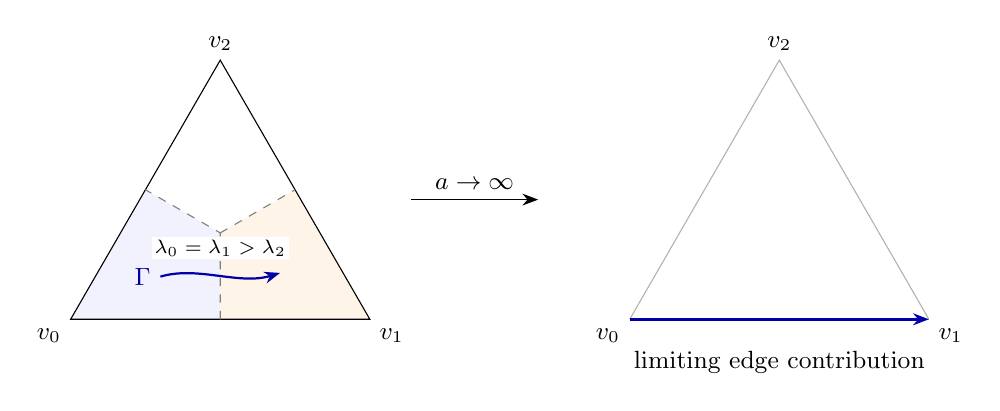
\begin{tikzpicture}[x=0.95cm,y=0.95cm,font=\small]
 \begin{scope}
  \fill[blue!5] (0,0)--(2,0)--(2,1.155)--(1,1.732)--cycle;
  \fill[orange!9] (4,0)--(3,1.732)--(2,1.155)--(2,0)--cycle;
  \draw (0,0)--(4,0)--(2,3.464)--cycle;
  \draw[dashed,gray] (2,0)--(2,1.155)--(1,1.732);
  \draw[dashed,gray] (2,1.155)--(3,1.732);
  \draw[blue!65!black,thick,-{Stealth[length=2mm]}]
    (1.2,0.57) .. controls (1.7,0.72) and (2.25,0.45) .. (2.8,0.62);
  \node[left,blue!65!black] at (1.2,0.57) {$\Gamma$};
  \node[below left] at (0,0) {$v_0$};
  \node[below right] at (4,0) {$v_1$};
  \node[above] at (2,3.464) {$v_2$};
  \node[font=\scriptsize,fill=white,inner sep=1pt] at (2,0.95)
    {$\lambda_0=\lambda_1>\lambda_2$};
 \end{scope}
 \draw[-{Stealth[length=2mm]}] (4.55,1.6)--(6.25,1.6)
    node[midway,above] {$a\to\infty$};
 \begin{scope}[xshift=7.1cm]
  \draw[gray!60] (0,0)--(2,3.464)--(4,0);
  \draw[blue!65!black,very thick,-{Stealth[length=2mm]}] (0,0)--(4,0);
  \node[below left] at (0,0) {$v_0$};
  \node[below right] at (4,0) {$v_1$};
  \node[above] at (2,3.464) {$v_2$};
  \node[below] at (2,-0.3) {limiting edge contribution};
 \end{scope}
\end{tikzpicture}
\caption{A two-dimensional model of a tie budget. Dashed segments
are the two-leader ties. The curve crosses one of them away from
the three-leader center; its image concentrates on the corresponding
edge. The right panel records the limiting contribution, not the
image under a finite-parameter homeomorphism.}
\label{lt:tie-model}
\end{figure}

For generic samples all relevant hits are finite on compact measured
pieces.  Higher ties, simplex-boundary junctions, and lower-dimensional
source exceptions are avoided by Lemma~\ref{lt:trace-slicing} and
translation coarea.  Counts consequently concern isolated hits at
regular underlying source strata; no differentiability of the original
image surface at such a hit is being assumed.

\subsection{A variable simplex squeeze}

\begin{lemma}[Compatible simplex squeezing]
\label{lt:squeeze}
Let $\mathcal T$ be a locally finite triangulation of a three-dimensional
open domain.  Assign constants $0<b_\sigma\leq1$ to its tetrahedra,
and to every nonempty face $\rho$ assign the minimum of the constants
of its incident tetrahedra.  On each tetrahedron put
\begin{align}
 b(\lambda)&=
 \min_{\varnothing\ne\rho\subseteq\sigma}
 \left(b_\rho+
        \frac{\max_{i\notin\rho}\lambda_i}{\max_j\lambda_j}\right),
       \label{lt:b-definition}\\
 a(\lambda)&=e^{1/b(\lambda)}-e,
 \qquad
 T_i(\lambda)=
 \frac{\lambda_i e^{a(\lambda)\lambda_i}}
             {\sum_j\lambda_j e^{a(\lambda)\lambda_j}},
       \label{lt:squeeze-definition}
\end{align}
where the maximum over an empty set in \eqref{lt:b-definition} is zero.
These formulas define a face-preserving, locally bi-Lipschitz
self-homeomorphism $T$ of the domain, with finitely many $C^1$ formulas
on closed pieces of every compact subset.  The normalized Lipschitz
constant of $b$ is bounded absolutely, independently of its minimum,
and a.e.
\begin{equation}
 |Da|\leq C(a+1)(1+\log(a+1))^2.
 \label{lt:a-derivative}
\end{equation}
If all the incident constants in a mesh neighborhood are one, $T$ is
the identity on its inner simplices.

Let $G$ parametrize finitely many compact $m$-traces, $m\in\{1,2\}$,
by finite closed-piece $C^1$ formulas, and suppose their intersections
with the $Z_{\sigma,I}$ are regular transverse hits away from higher
ties and simplex boundaries.  Every counted hit is in the interior
of each counted regular $m$-dimensional parameter branch; parameter
boundaries and lower-dimensional parameter strata avoid the counted
dual strata.  As the lower bounds of $a$ tend to
infinity on the measured neighborhood,
\begin{equation}
 \int J_mD(T\circ G)
 \longrightarrow
 \sum_{\text{hits on }Z_{\sigma,I}}
       \cH^m(\conv\{v_i:i\in I\}),
 \label{lt:squeeze-area}
\end{equation}
with multiplicity.  The local convergence, and in particular its upper
bound with arbitrarily small error, is uniform when other floors of
$a$ are made arbitrarily larger.  Continuous weights may be bounded
by their simplex suprema in this conclusion.
\end{lemma}

\begin{proof}
Since the candidate $\rho=\sigma$ gives $b\leq b_\sigma\leq1$,
$a\geq0$.  Every denominator $\max\lambda_j$ is at least $1/4$,
so the normalized Lipschitz constant of $b$ is absolute.  The chain
rule gives \eqref{lt:a-derivative}.  On a face $\tau$, replacing a
candidate $\rho$ by $\rho\cap\tau$ leaves its nonzero outside
coordinates unchanged and can only lower its constant, because
$b_{\rho\cap\tau}\leq b_\rho$.  An empty intersection gives an
outside-coordinate ratio of one and cannot improve on $b_\tau\leq1$.
Thus restrictions agree on faces.  Positivity, zero coordinates, and
the order of coordinates are preserved by \eqref{lt:squeeze-definition}.

We verify invertibility even though $a$ is variable.  Given output
ratios $z_i=T_i/T_{\max}\in[0,1]$, for a trial $D\geq0$ let $r_i$
be the unique solution of
\begin{equation}
 z_i=r_i e^{-D(1-r_i)},\qquad 0\leq r_i\leq1.
 \label{lt:ratio-inverse}
\end{equation}
The function of $r_i$ on the right is strictly increasing.  Each
$r_i$ is nondecreasing in $D$, with the zero and maximal ratios fixed
at zero and one.  Put $R=\sum_i r_i$ and $\lambda_i=r_i/R$.
The trial value of $a$ is $DR$, an increasing function of $D$ with
increase at least that of $D$.  In \eqref{lt:b-definition} the
outside-coordinate ratios are exactly $r_i$; hence $b$ at this trial
inverse is nondecreasing in $D$.  Its prescribed value
$e^{1/b}-e$ is nonincreasing.  The equation
\[
 DR=e^{1/b(\lambda)}-e
\]
has a unique solution, by continuity, its sign at $D=0$, and its
positive sign for large $D$.  This proves bijectivity.
On an individual closed simplex $b$ has a positive lower bound, so
the solution has bounded $D$.  Equation~\eqref{lt:ratio-inverse}
has uniformly Lipschitz inverse in this bounded range, including at
zero output coordinates.  The scalar equation's left-minus-right
increase is at least the increase in $D$, so its root depends
Lipschitz-continuously on the output.  Since $T_{\max}\geq1/4$,
forming the output ratios is Lipschitz as well.  The forward formula
is Lipschitz on that simplex, and its inverse is Lipschitz.  The
finite min/max alternatives in \eqref{lt:b-definition} give finitely
many closed pieces with $C^1$ extensions of the formulas.  Local
finiteness proves all the global assertions.  If the incident
constants are one, the minimum is one, so $a=0$ and $T=\Id$.

It remains to prove the concentration assertion.  On a compact trace
set away from $(m+1)$-fold leader ties, at most $m$ coordinates can be
near the maximum.  Coordinates outside that set and all their
derivatives are exponentially small in $a$, multiplied only by
powers of $a$ and $\log(a+e)$ by \eqref{lt:a-derivative}.  The active
coordinates have total mass one up to those errors and therefore
take values in a face of dimension at most $m-1$.  Their $m$-Jacobian
vanishes.  Expanding the actual $m$-Jacobian then shows uniform
convergence to zero away from the counted ties, including along
simplex faces by the same piecewise calculation.

Near a transverse hit relabel the leaders $0,\ldots,m$ and use
\[
 u_i=\lambda_i-\lambda_0,\qquad 1\leq i\leq m,
\]
as trace coordinates.  All leader coordinates have a fixed positive
lower bound there, and the remaining coordinates are separated below
them.  Normalize the probabilities on the leaders first.  Their
logit differences are
\[
 a(u)u_i+\log\frac{\lambda_i(u)}{\lambda_0(u)}.
\]
Inactive probabilities and derivatives are exponentially small.
Write $a_0=a(0)$.  Since
$b(0)=1/\log(a_0+e)$ and $b$ is uniformly Lipschitz, on
$u=t/a_0$ with bounded $t$ one has
\[
 \log\frac{a(u)+e}{a_0+e}
       =O\left(\frac{(\log(a_0+e))^2|t|}{a_0}\right)=o(1).
\]
The scaled derivative terms coming from $Da$ tend to zero by
\eqref{lt:a-derivative}.  The leader map and its a.e. derivatives
therefore converge locally uniformly, apart from its harmless
piece seams, to
\[
 t\longmapsto
 \left(\frac{e^{t_i}}{1+\sum_{j=1}^m e^{t_j}}\right)_{i=1}^m.
\]
This softmax map is a diffeomorphism from $\R^m$ onto the interior
of the standard $m$-simplex.  Multiplication by the physical edge
vectors consequently gives exactly the flat $m$-area of the leader
face, provided the tails vanish.

Here are uniform tail bounds.  The determinant of the active
probability derivative is its probability product times the
determinant of the logit derivative.  The logit derivative has the
form $aI+u\otimes Da+B$, with $B$ bounded for the fixed trace chart.
The probability product is at most $C e^{-ca|u|}$.  Thus the
absolute determinant, modulo exponentially small inactive terms,
is bounded by
\begin{equation}
 C(1+a+|Da|\,|u|)^m e^{-ca|u|}.
 \label{lt:tail-bound}
\end{equation}
For $|u|\leq a_0^{-1/2}$, the preceding logarithmic estimate is
uniform and gives $a/a_0\to1$ there.  After scaling, the
determinant has an integrable bound $Ce^{-c|t|}$, because
$|Da||u|/a_0\leq C(\log a_0)^2a_0^{-1/2}=o(1)$.
For
\[
 a_0^{-1/2}<|u|\leq c_1/\log(a_0+e),
\]
choose $c_1$ small relative to the fixed Lipschitz bound for $b$.
Then $a\geq a_0^{3/4}$ for large $a_0$, and
$a|u|\geq a_0^{1/4}$.  Exponential decay in
\eqref{lt:tail-bound} absorbs all polynomial and logarithmic
factors uniformly for every larger $a$.
In the remaining sufficiently small neighborhood,
\[
 b(u)\leq b(0)+C|u|\leq C'|u|,
 \qquad a(u)+e\geq e^{c'/|u|}.
\]
For small $r=|u|$, the expression $a^N e^{-car}$ is decreasing
once $a\geq e^{c'/r}/2$, for any fixed $N$.  Increasing $N$ to
absorb the logarithms in \eqref{lt:tail-bound} therefore gives an
integrable bound of the form
\[
 C\exp(Nc'/r)\exp(-c''r e^{c'/r}),
\]
independent of how high the local floors are.  At every fixed
$u\ne0$ the integrand tends to zero as the floor tends to infinity.
Dominated convergence treats this last region.  These three bounds
prove tail vanishing and \eqref{lt:squeeze-area}.

For a compact measured list there are only finitely many charts and
hits.  One may therefore prescribe the floors simultaneously, with
any allocated small errors.  Local finiteness then permits such
choices for a locally finite list, including summable errors.  The
map moves a point only inside its own simplex, so multiplication by
simplex suprema of continuous weights proves the weighted upper
bound.  The same reasoning applies to every regular parameter
branch, and hence respects multiplicity.
\end{proof}

\subsection{Transfer and selection of the budgets}

\begin{proposition}[Topological transfer of trace budgets]
\label{lt:budget-transfer}
Fix generic trace data as in Lemma~\ref{lt:trace-slicing} and a
sufficiently fine generic mesh from Lemma~\ref{lt:target-mesh}.
There is an onto locally bi-Lipschitz homeomorphism
$H_0:\Omega\to\Omega'$, locally specified by finitely many
$C^1$ formulas on closed pieces, whose image lengths and areas on
the measured traces are at most their tie budgets plus arbitrarily
small prescribed local errors.  Nonnegative continuous output
weights are allowed, with the simplex-supremum budgets of
Definition~\ref{lt:tie-budget}.

The map can be arbitrarily close to $f$, with reciprocal closeness
on interior compact sets, within the mesh displacement and chosen
local modification errors.  It can retain smaller exact affine
germs previously installed at a locally finite family of crossings
and finitely many star centers, and can retain strict compact
forward and inverse safety conditions, including angular cone
conditions, whenever they have positive margins.  For this relative
usage, measured data are separated from buffered open exemptions
around the protected germs: a measured trace either avoids the
exempt cores, or its weight vanishes there with a buffer.  Every
germ required to remain exact in $H_0$ is contained in one of these
buffered exemptions.  The affine crossing germs installed at the
newly cleaned measured hits are retained only in the intermediate
map $G$ for the concentration calculation; no affine-germ condition
at those hits is imposed on $T\circ G$.  The mesh and all measured
configurations are fixed before the squeezing floors are selected.
\end{proposition}

\begin{proof}
Each area-line hit is an isolated intersection of the image of a
regular source surface with an affine target interval.  Apply
Lemma~\ref{lt:clean-crossing}, then Corollary~\ref{lt:affine-crossing},
in a paired source and target neighborhood.  For a curve-plane hit,
interchange source and target and clean the preimage plane.  The
supports can be chosen disjoint and locally finite.  Area-line hits
avoid curve-plane hits and the measured curve images; curve-plane
changes can avoid all area-test lines.  If parametrizations share a
regular source stratum at a hit, the operation is performed once on
that stratum and its fixed multiplicity is retained.  Lower strata
and other sheets are absent there by genericity.  A surviving hit
remains in its intended source stratum and target tie simplex, and
the cleaning does not increase its count.

Use Lemma~\ref{lt:relative-germs} to obtain a locally bi-Lipschitz
map $G$ with finite closed-piece $C^1$ formulas, keeping smaller
exact crossing and center neighborhoods.  Take the approximation
smaller than the positive gaps from all forbidden strata off those
neighborhoods.  The measured intersections of $G$ are now regular
transverse intersections and their counts do not exceed the
original budget counts.  Choosing all supports and approximation
errors finely also retains the stated compact forward and inverse
conditions.  These choices use only topology and qualitative
approximation; no derivative bound for $G$ is charged to a budget.

Apply Lemma~\ref{lt:squeeze} in the target and set $H_0=T\circ G$.
It has the asserted local regularity and is an onto homeomorphism.
On each compact measured list choose the floors high enough that
the image measurements cost at most the flat weights plus their
allocated errors.  Finitely many such lists meet each simplex, so
the uniformity in arbitrarily higher floors permits simultaneous
choices for the locally finite family.

For the relative assertion, first keep each protected-germ modification
deep inside its exempt region.  Make the mesh so fine that all
simplices touching the protected no-movement core, and their needed
neighbors, lie inside that exemption.  Assign the value one to
their $b_\sigma$ constants; then $T=\Id$ on a smaller neighborhood
of the germ.  All simplices required for measured points, including
points where the final weight is nonzero, remain buffered away
from these cores and use the original $f$-crossings.  Subsequent
cleaning supports are disjoint from the core neighborhoods.
Every motion by $T$ stays inside a simplex.  Thus the chosen fine
mesh retains the strict margins and the reciprocal compact
accuracies, and $w(TG(x))\leq\sup_\sigma w$ whenever $G(x)\in\sigma$.
This proves the weighted estimate as well.  No unweighted estimate
through an exempt affine-star core is asserted or needed.
\end{proof}

\begin{lemma}[Expected budgets]
\label{lt:budget-expectation}
For an $m$-trace with finite image measure, the meshes in
Lemma~\ref{lt:target-mesh} satisfy
\begin{equation}
 \mathbb E\,\mathcal B_m(\Gamma)
             \leq C\int_K J_mD(f\circ P),
 \label{lt:expected-budget}
\end{equation}
with parameter multiplicity understood.  The constant is universal
outside enlarged lattice patches and may depend on their fixed
aspect ratios inside them.  The estimate holds locally with
comparable enlargements.  For continuous weights it holds with
the weighted trace integral and an arbitrarily small enlargement
error as the local mesh sizes tend to zero.  Fixed linear output
normalizations may be included in all areas.
\end{lemma}

\begin{proof}
Use the joint variables $(t,z)$ of
\eqref{lt:mesh-joint-density} for a candidate tetrahedron.
For each fixed $z$, its dual $(3-m)$-piece $Z_z$ has diameter
$O(d)$ and measure at most $Cd^{3-m}$; translation by $t$
produces the actual dual piece.  If $N(t,z)$ is its intersection
count with the measured trace in the candidate's fixed enlarged
neighborhood, translation coarea gives
\[
 \int N(t,z)\,dt
 \leq C d^{3-m}\,
          \text{local trace image $m$-measure}.
\]
Indeed this is the area formula for the difference of the trace
and dual-piece parametrizations, whose angle factor is at most one.
The joint density bound therefore gives, for every such $z$,
\[
 \int q(t,z)N(t,z)\,dt
 \leq C d^{-m}\,
          \text{local trace image $m$-measure}.
\]
These are unnormalized translation integrals.  Integrating $z$
over its bounded normalized set only changes the constant.
The flat $m$-face weight is at most $Cd^m$ for every $z$, so it
cancels the remaining scale.  Discard the Delaunay selection
indicator for this upper estimate.
Only boundedly many candidate tuples occur locally and their
enlargements have bounded overlap, proving
\eqref{lt:expected-budget}.  The same coarea calculation gives
generic avoidance of negligible sets and finiteness of compact
counts.  A continuous weight's supremum on each vanishing simplex
differs from its value at a measured point by its local modulus
of continuity.  On a compact set multiply that modulus by the
finite trace measure; a locally finite exhaustion and allocated
errors give the weighted assertion.
\end{proof}

\begin{lemma}[Length budgets with arbitrarily high probability]
\label{lt:curve-probability}
For any compact rectifiable measured curve $\Gamma$ of finite
length, any $\delta>0$, and any $e>0$, sufficiently small local
mesh upper bounds make
\begin{equation}
 \mathcal B_1(\Gamma)\leq C\operatorname{length}(\Gamma)+e
 \label{lt:curve-high-probability}
\end{equation}
hold with probability at least $1-\delta$.  The constant $C$ is
independent of $\delta,e$ and the required mesh resolution; it is
universal away from enlarged patches.  Prescribed summable failure
probabilities and local errors can be imposed simultaneously on a
countable locally finite family of curves.  In a deep anisotropic
lattice patch there is also a grid-unit version: rescale to unit
grid aspect, estimate length there, and convert the weight back
using the longest physical side, with a constant independent of
the aspect ratio in those units.
\end{lemma}

\begin{proof}
Discard an arbitrarily small amount of length with multiplicity
and decompose the remainder into finitely many compact pieces on
$C^1$ graphs of arbitrarily small slope $s$ over straight axes.
Such pieces may be taken injectively from the regular parameter
branches, so multiplicity is accounted for by separate pieces.
Cover their axis projections by finitely many intervals of total
length at most the sum of their graph-piece lengths plus an
arbitrarily small error.  Extend the graphs over these intervals
with comparably small slopes.

For each fixed relative-coordinate value $z$ in the joint
integration formula \eqref{lt:mesh-joint-density}, classify a dual
plane by its unit normal $\nu(z)$ and the graph axis $e$.  If
$|\nu\cdot e|>2s$, the restriction of its affine defining function
to the graph is strictly monotone.  Each such plane patch meets
the graph over its interval at most once.  Charge a contributing
tetrahedron to an axis interval of length comparable to $d$
centered at a hit.  Intersecting charged intervals have comparable
scales, by slow grading, and their vertices belong to a bounded
local candidate list.  Thus the charges have bounded overlap.
The sum of mesh diameters, and hence of the flat edge weights,
is bounded by a constant times the graph length plus the local
mesh upper bound at each interval endpoint.  After the finite
cover is fixed, all endpoint overhangs can be made as small as
desired by the mesh choice.

For the remaining normals, the translation-coarea factor on this
graph is at most $Cs$.  For each fixed $z$, integration over the
physical translation variable bounds the crossing integral by
$Cs d^2$ times the local graph length.  Multiply by the joint
density bound $Cd^{-3}$ and the edge weight $Cd$, and then
integrate over the bounded relative-coordinate set.  This gives
expected cost at most $Cs$ times the graph length.  The normal
classification is translation invariant, so it is legitimate
inside this unnormalized joint integral.  The omitted trace length has correspondingly
small expected cost by Lemma~\ref{lt:budget-expectation}.  Choose the omitted length
and $s$ sufficiently small, then choose the mesh bounds for the
finite graph cover.  Markov's inequality applies only to these
small remainders, and makes their failure probability below
$\delta$ without changing the constant on the retained graph
length.  This proves \eqref{lt:curve-high-probability}.

For a locally finite family assign summable failure probabilities
and errors and impose the corresponding local upper bounds
together.  A union bound proves the simultaneous assertion.
In a deep lattice patch perform the entire argument after the
anisotropic rescaling.  There are finitely many rational tie-plane
families in these units; the same argument, or translated Riemann
sums for their projected length coarea, gives the claimed constant.
Physical flat weights are bounded by the longest-side factor
times their grid-unit weights.
\end{proof}

\begin{lemma}[Sharp costs along a thin-grid subspace]
\label{lt:sharp-grid}
In a deep lattice patch adapted to a fixed $k$-plane $E$, use side
$d$ along $E$ and side $\eta d$ along $E^\perp$, where
$k\in\{1,2\}$.  For $m=k$, the translation-averaged tie-budget
coefficient on a simple $k$-vector tangent to $E$ is at most
$1+C\eta$ times its Euclidean norm.  For general measured
$m$-vectors, tangent contributions have constants uniform in
$\eta$, and errors have a finite constant $C_\eta$.
After a fixed linear output normalization $A$ which keeps the two
subspaces orthogonal, the sharp coefficient relative to the normalized
tangent length or area is at most $1+C_A\eta$. Here $C_A$ depends only on
$\|A\|_{\op}$ and $\|A^{-1}\|_{\op}$. The tangent bounds remain
uniform in $\eta$, while the error constants may also depend on these
two norms.
The grid-unit bound of Lemma~\ref{lt:curve-probability} also has no
aspect-dependent factor on tangent lengths.
\end{lemma}

\begin{proof}
Rescale the grid to unit cubes, temporarily recording physical
flat weights separately.  For $k=2$ slice a cube at a generic
height in its thin direction.  Each Kuhn tetrahedron projects to
a triangle with one repeated vertex.  Write the two unsplit
projected barycentric masses as $q_s,q_t$.  On a fixed-height
slice, either part $\lambda_0$ of the split mass is a constant
minus a sum of some of $q_s,q_t$, with coefficients zero or one.
Consequently
\[
 \det D_{(q_s,q_t)}(q_s-\lambda_0,q_t-\lambda_0)>0.
\]
These are also the orientation coordinates for a leader triangle
with three different projected vertices.  Thus every such
projected triangle is counted positively.

The total projected weight on a horizontal period is exactly
its area.  One way to see this without estimating individual
positions is to take a constant large $a$ in
\eqref{lt:squeeze-definition}.  Projection of this periodic
simplexwise map on the horizontal slice is a torus map with
periodic displacement and degree one.  Its signed Jacobian
integrates to one base area.  Lemma~\ref{lt:squeeze} converts
this integral, in the large-$a$ limit, into the signed projected
triangle weights.  Generic heights give only finitely many
transverse hits away from simplex boundaries; the signs just
computed are positive, and repeated projections contribute zero.
For a direct check, the two Kuhn tetrahedra whose vertical step
comes first supply total projected area one at heights
$2/3<z<1$, those whose vertical step is middle supply one for
$1/3<z<2/3$, and those whose vertical step is last supply one for
$0<z<1/3$.  Each nondegenerate leader triangle contributes $1/2$
at its applicable height.  The finitely many exceptional heights
do not affect translation averaging.

In physical units a nondegenerate projected triangle differs
from its projected area by at most $C\eta$ times the base area;
a triangle with repeated projections has area at most
$C\eta d^2$.  The number of hits per period is uniformly bounded.
The total physical area cost is therefore at most
$(1+C\eta)d^2$.

For $k=1$, fix generic coordinates transverse to the long axis
and traverse one axial period.  Within a Kuhn tetrahedron the
varying barycentric pair transfers mass from its lower axial
position to its upper axial position, while the other masses
are fixed.  A switch between leaders with different axial
projections is consequently always forward.  Two fixed
unsplit masses do not tie at a generic transverse coordinate.
The projected periodic map has degree one, so total projected
length is exactly the axial period.  Edges with equal axial
projection, and the transverse parts of the other edges, cost
only $O(\eta)$ in period units.  This proves the sharp length
coefficient.

Translation coarea expresses each coefficient on a trace
Jacobian as a finite homogeneous sum of absolute linear forms
on its $m$-vector.  The parallel-vector computations therefore
give the asserted tangent coefficients.  Splitting a vector
into its tangent part and its error and using the triangle
inequality gives a finite $C_\eta$ on the error.  A fixed
normalization preserving orthogonality of the two subspaces
changes these constants only through its two norm bounds.
The final length assertion follows by making the anisotropic
rescaling before applying Lemma~\ref{lt:curve-probability}.
\end{proof}

\begin{remark}[Order of choices for weighted budgets]
\label{lt:weighted-order}
Additional compact configurations and continuous weights may be
fixed before selecting the target mesh bounds.  They change how
fine the mesh must be for the preceding estimates, but not the
constants in those estimates.  Small open exemptions, their
buffered no-movement cores, and strict angular safety conditions
are included in this convention.  Squeezing floors are selected
only after the regular transverse map $G$ and its compact
measurement lists are fixed.
\end{remark}

\subsection{Source meshes with uniform shapes}

\begin{lemma}[Shape-controlled source sampling]
\label{lt:source-mesh}
There are locally finite source meshes of uniform shape with
arbitrarily small local upper size bounds, preserving finitely
many separated deep cubical lattice patches in prescribed
orientations and with prescribed common fine scales.  Deep
cells may remain cubes; elsewhere they are tetrahedra, with
matching facet diagonals at interfaces.  For an integrable
nonnegative function $g$ and $m\in\{1,2\}$, their sampled
$m$-faces satisfy the local estimate
\begin{equation}
 \mathbb E\sum_F \ell_F^{3-m}\int_F g\,d\cH^m
                    \leq C\int g,
 \label{lt:source-fubini}
\end{equation}
with comparable local enlargements and bounded overlap understood.
In particular this applies to $g=|Df|^p$ and controls the
tangential derivative trace integrals.  Lattice shifts can also
be uniform over any prescribed macro-period formed by grouping
fine cubes.
\end{lemma}

\begin{proof}
Use the construction of Lemma~\ref{lt:target-mesh}, now with
cubical rather than anisotropic deep patches, and impose
uniform altitude avoidance on the unstructured sites.  Conditional
on the lattice shifts, enumerate these sites and place them
successively.  When placing a site, exclude a neighborhood of
thickness $\varepsilon_0$ times its scale around the affine span
of every nearby tuple of at most three earlier or lattice
vertices.  Candidate neighbor lists are fixed and bounded by
localization.  A neighborhood of each such plane, line, or
point removes at most $C\varepsilon_0$ of the jitter volume.
For an absolute sufficiently small $\varepsilon_0$, at least
half the jitter volume remains.  Choose uniformly in the
remaining portion.

Any affinely independent lattice prefix of a candidate simplex
comes from one rotated cubical lattice.  There are only finitely
many relevant normalized configurations, so its nonzero
determinant or lower-dimensional volume has an absolute lower
bound.  Each subsequently placed vertex has altitude at least
$\varepsilon_0$ times scale over the affine span of the preceding
vertices.  Induction gives a uniform lower bound on every
nondegenerate simplex determinant after scaling.  Together with
the upper diameter bound this gives uniform shapes.  Fully
lattice simplices have the usual finite collection of Kuhn
shapes.  Deep cells may be left cubical, using the same
diagonals on shared facets when meeting triangulated cells.
Block modifications can consequently be kept inside cubical
regions, with whole shared squares on their outer boundaries.

Given the previously placed sites and the lattice shifts, each
new jitter has conditional density at most twice its original
uniform density.  Successive integration of the unselected sites,
or the corresponding iterated-expectation bound on rectangular
events, therefore bounds the joint density of any fixed tuple of
$k$ selected unstructured sites by $C^k d^{-3k}$, uniformly in
the lattice shifts.  The jitters need not be independent.  Include the uniform density of a candidate's lattice shift, if
present, and make the same change of variables as in
Lemma~\ref{lt:target-mesh}.  This again gives a joint density
$q(t,z)\leq Cd^{-3}$ for physical translation and normalized
relative coordinates.  Discard any later selection indicator.
For each fixed $z$, an $m$-face has area $O(d^m)$, and Fubini gives
\[
 \int dt\int_{t+F_z}g\,d\cH^m
       \leq Cd^m\int_{U}g,
\]
where $U$ is the candidate's comparable enlarged neighborhood;
only translations in its bounded support are included on the
left.  Multiplying by $Cd^{-3}$, then integrating $z$ over its
bounded set, gives $Cd^{m-3}\int_U g$ for the expected face
integral.  Its mesh scale is comparable to $d$ by shape control.
Multiplication by $\ell_F^{3-m}$, followed by bounded candidate
counts and overlap, proves \eqref{lt:source-fubini}.

For grouping fine cubes into macro-cubes, choose independently
a uniform fine-period shift and a uniform discrete grouping
offset.  Their sum is uniform over the macro-period.  Truncation
of a lattice list concerns sites inside its fixed buffered patch;
it does not translate the transition-site lists by many mesh
steps.  Thus every mixed local candidate still uses only one
fine-scale physical translation variable after subtracting that
shift and normalizing its jitter coordinates.  Its bounded joint
density, and hence the unnormalized joint Fubini calculation,
remain unchanged.
\end{proof}

\section{Approximation for the low exponents}\label{sec:low-assembly}

We prove the approximation theorem for $1\le p\le2$.  The local
constructions in this section use the curve and surface budgets of the
preceding section.  Surface budgets, and the inverse-$BV$ theorem, are
used only when $p=2$.

\begin{theorem}[Low-exponent approximation]\label{la:approximation}
Let $\Omega,\Omega'\subset\R^3$ be bounded domains, let $1\le p\le2$, and
let $f:\Omega\to\Omega'$ be a homeomorphism in
$W^{1,p}(\Omega;\R^3)$.  For every $\eps>0$ there is a locally
bi-Lipschitz homeomorphism $H:\Omega\to\Omega'$ such that
\begin{equation}\label{la:goal}
 \int_\Omega \bigl(|H-f|^p+|DH-Df|^p\bigr)<\eps.
\end{equation}
In particular, the target of $H$ is exactly $\Omega'$, and
$H\in W^{1,p}(\Omega;\R^3)$.
\end{theorem}

We work on finitely many compact sets carrying controlled jets.
At rank three, radial blocks recover those jets; at ranks one and two,
kernel compression reduces the core estimate to a line or plane section,
with a further planar radial construction at rank two when $p<2$.
Boundary parametrization completes the remaining cells, and the final
proof records the order of choices and proves global summability.

Throughout the section, all modifications are made inside the open
domains.  Constants denoted by $C$ depend only on the dimension, $p$,
and the fixed shape constants.  A subscript records any additional
dependence.  In an expression $o(1)$ involving a mesh size, all the
other parameters and the finite compact configuration have already
been fixed.  The quantities tending to zero will always be
nonnegative costs or upper bounds for such costs.

\subsection{Composition at a collapsed stratum}

We first record the regularity fact used when a three-dimensional
region is compressed toward a line or a plane.  It also explains why
the finite-piece regularity in the budget construction is retained.

\begin{lemma}[Tangential composition limit]\label{la:composition-limit}
Let $D$ be a compact Lipschitz parameter piece of dimension $d$, and let
$q_j,q_0:D\to U$ be Lipschitz maps into an open subset of a Euclidean
space.  Suppose that their images lie in one compact subset of $U$,
that $q_j\to q_0$ uniformly, and that
\[
 Dq_j\longrightarrow Dq_0\quad\hbox{a.e. on }D,
 \qquad \sup_j\|Dq_j\|_{L^\infty(D)}<\infty.
\]
Let $v:U\to\R^a$ be Lipschitz on a neighborhood of that compact set.
Suppose there are finitely many closed pieces $C_\nu$ covering the
neighborhood and $C^1$ maps $v_\nu$, defined on neighborhoods of
$C_\nu$, such that $v=v_\nu$ on $C_\nu$.  Then, for every finite
$r\ge1$,
\begin{equation}\label{la:composition-convergence}
 D(v\circ q_j)\longrightarrow D(v\circ q_0)
       \quad\hbox{in }L^r(D).
\end{equation}
No rank assumption is imposed on $Dq_0$.  The assertion applies
separately to an edge, a face, or a volume piece.
\end{lemma}

\begin{proof}
For each $j\ge0$ and each $\nu$, apply the density theorem on the
parameter piece to $q_j^{-1}(C_\nu)$.  At almost every point of this
preimage, locality of the weak derivative gives
\[
 D(v\circ q_j)=Dv_\nu(q_j)Dq_j.
\]
Remove the union of the exceptional sets for the countably many $j$
and finitely many $\nu$.  At a remaining parameter point, every branch
containing $q_0$ gives the same product with $Dq_0$, namely
$D(v\circ q_0)$.  If a branch occurs along infinitely many $q_j$, its
closedness implies that it contains $q_0$.  Continuity of its
derivative and convergence of $Dq_j$ therefore show that its products
converge to this common value.  Finiteness of the branch list proves
pointwise convergence of the full sequence.  The fixed derivative
bounds give a bounded majorant, so dominated convergence proves
\eqref{la:composition-convergence}.  The proof takes place on $D$;
it does not pull back an ambient null set through a possibly
rank-deficient map.
\end{proof}

\subsection{Full-column-rank radial blocks}

Here the parameter dimension is either $m=3$, with $1\le p\le2$, or
$m=2$, with $1\le p<2$.  In the latter case the parameter domain is a
flat plane section of the source.  All target motions remain ambient
three-dimensional homeomorphisms.

Let $K$ be a compact subset of such a parameter patch.  Assume that
there is a local $C^1$ ambient diffeomorphism $b$ such that
\begin{equation}\label{la:identity-jets}
 f=b,\qquad D_m f=D_m b\quad\hbox{on }K
\end{equation}
up to the null sets of the indicated traces.  The map $f$ on the patch
is Sobolev and has its continuous ambient values.  Both $Db$ and
$(Db)^{-1}$ are bounded by a fixed constant, denoted collectively by
$C_b$.  For $m=2$, the additional normal column of $b$ is chosen so
that its ambient orientation agrees with that of $f$.
Write
\[
 F=b^{-1}\circ f.
\]
Thus $F=\Id$ and $D_mF=I_m$ on $K$, where $I_m$ is the derivative
of the identity inclusion of the parameter plane into $\R^3$.
Target coordinates in the following construction are always the
$b$-coordinates.  If $m=3$ and $p=2$, then
\begin{equation}\label{la:inverse-bv}
 F^{-1}\in BV_{\mathrm{loc}},
\end{equation}
by \cite[Theorem~1.1]{CsornyeiHenclMaly2010}.  That theorem requires no
finite-distortion hypothesis.

Choose an integer $N$, put $l=N^{-1}$, and fix a sufficiently large
absolute constant $K_0$.  Set
\begin{equation}\label{la:gamma}
 \gamma=l/K_0.
\end{equation}
Use a uniformly shifted cubical grid of side $h$, with each macro cube
subdivided into tiles of side $lh$.  The word ``cube'' includes a
square when $m=2$.  Cubes meeting $K$ are candidates.  In each candidate
$Q$, draw a center $a$ uniformly in a central cube of side $h/4$; retain
only centers belonging to $K$.  Rays from $a$ through boundary mesh
vertices are the forward spokes.  When $m=3,p=2$, also choose,
independently on each boundary mesh square, a point $u_j$ uniformly in
its central half and use the target ray from $a$ through $u_j$.

Cubical polar coordinates are written
\[
 x=a+r(\omega-a),\qquad \omega\in\partial Q,
\]
so the boundary has radial coordinate $r=1$.  In dimension two, the
ambient output box is the normal thickening of $Q$, centered on the
parameter plane and of height $h$.

\begin{lemma}[Radial block construction]\label{la:radial-blocks}
Fix finitely many separated compact configurations satisfying
\eqref{la:identity-jets}, and fix $l$.  For sufficiently small $h$ one
can retain candidate blocks with the following properties.

\begin{enumerate}
\item The expected $m$-volume of discarded candidate blocks tends to
zero as $h\to0$.  The union of retained blocks therefore differs
from $K$ by a set whose expected measure tends to zero.
\item Each retained $Q$ has the core
\[
 B_Q=a+(1-8\gamma)(Q-a).
\]
The complement consists of shape-controlled frusta of scale $lh$, one
over each boundary tile.  After the common budget construction and
the source and target changes described below, the map on $B_Q$ is
$b$, except on caps of total measure at most $C\gamma |Q|$.  Its
tangential derivative on the whole core and its core boundary is
bounded by $C_b$.
\item Every radial connector in the final shell has image length at
most $C_b\gamma h$.  Nonincident mesh edges avoid the radial-angular
expansions.  Subsequent cap contractions multiply their length
budgets by at most a fixed constant.  With $\ell=lh$, the converted
shell edge cost after constant-speed parametrization is
$\ell^{m-p}\sum_e L_e^p$, where $L_e$ is the image length.
Its bound is $O_b(l)\sum_Q|Q|+o(1)$ after the source selection and
individual curve-budget bounds, with arbitrary additional transfer
errors.
\item If $m=3,p=2$, include the full wedge from $a$ to each boundary
tile edge among the measured surfaces.  There are bounded continuous
weights, fixed before the target budget mesh, for which the final
connector-face areas are bounded by the weighted $H_0$-areas, up to
arbitrarily small errors.  After multiplication by $lh$, the expectation of their total converted budget
$\mathcal B_{\mathrm{wedge}}$ satisfies
\begin{equation}\label{la:wedge-cost}
 \mathbb E\mathcal B_{\mathrm{wedge}}
       \le C_b\gamma\sum_i |K_i|+o(1).
\end{equation}
Outer ordinary edges and faces have converted cost
$O_b(l)\sum_Q|Q|+o(1)$ on these configurations.
\end{enumerate}
The construction can be performed simultaneously with the other
budgeted pieces used below.  In a volume block the only measured
interior surfaces are its wedges.  In the plane-section application,
any additional graph to be fixed is assumed to have positive
clearance from $K$ and its image.  Taking $h$ smaller then keeps all
expansion and cap supports off that graph.  More precisely, write
$V$ for the ambient initial map after its output motions and
$q_Q:Q\to Q$ for the radial parameter change.  The controlled trace
is $V\circ q_Q$.  For $m=3$ these parameter changes are ambient
source self-homeomorphisms; for $m=2$ they are retained solely as
section parametrizations.  The graph preservation means that the
radial motions leave its already-budgeted $H_0$-image unchanged;
it does not assert equality of $H_0$ with $f$ on that graph.
\end{lemma}

\begin{proof}
We give the selection, the maps, and the estimates in their order of
use.

\paragraph{Selection of centers and stars.}
Averaging the macro shift and the center draw is equivalent, up to
fixed bounded densities, to integration in the actual center $a$ and
normalized relative offset variables.  The weight in a block sum is
$h^m$.  Failure to choose $a\in K$ on candidate blocks costs at most
\[
 C\bigl|N_{Ch}(K)\setminus K\bigr|,
\]
which tends to zero.  Here $N_t(K)$ denotes the parameter-space
$t$-neighborhood of $K$.

For almost every center in $K$ and almost every fixed choice of
relative variables, each of the finitely many forward line traces is
absolutely continuous and has derivative the identity at $a$ in the
one-dimensional Lebesgue-point sense.  This follows from slicing and
$D_mF=I_m$ on $K$.  In the reverse system, use
\eqref{la:inverse-bv} and $F^{-1}=\Id$ on $K$, together with directional
$BV$ slicing and its separate absolutely continuous and singular
variation identities
\cite[Section~3.11, Theorems~3.103, 3.107, and~3.108]{AmbrosioFuscoPallara2000}.
At almost every line
density point of $K$, the absolutely continuous derivative of the
inverse trace is the identity and the density of its singular
variation is zero.  The trace is continuous because $F^{-1}$ is
continuous.  Consequently both systems have relative conical
differentiability at $a$, and the length of an initial ray interval is
its radius times $1+o(1)$.

For completeness, near-minimal length gives the single-crossing
sections required by Proposition~\ref{lt:star}.  The radial distance along
one distorted initial ray attains every level up to $(1-o(1))t$ and
has total variation at most $(1+o(1))t$.  One-dimensional coarea shows
that levels with more than one crossing have measure $o(t)$.  A finite
union of these exceptional sets still has measure $o(t)$, so there
are arbitrarily small common levels crossed once by every ray in
the system.  Injectivity and the local differentiability estimate
exclude remote tails from these shrinking sections.

The loop condition in Proposition~\ref{lt:star} is also obtained by slicing.
Fix one of a countable library of finite piecewise smooth loop
systems on the angular sphere.  For a fixed library loop $\omega$, set
\[
 E_t(a)=\int\bigl(|D_mF(a+t\omega(s))-I_m|^p
       +\mathbf1_{\text{patch}\setminus K}(a+t\omega(s))\bigr)
                         |\omega'(s)|\,ds.
\]
Extend the integrands to a fixed neighboring patch.  Translation
continuity and their vanishing on $K$ give
$\int_K E_t(a)\,da\to0$.  A diagonal choice of $t_n\downarrow0$
with summable means for the first $n$ library loops gives
$E_{t_n}(a)\to0$ for every loop at almost every center.  Each loop
then has a point in $K$, where $F=\Id$.  Absolute continuity from
that point gives uniform convergence of
$(F(a+t_n\omega)-a)/t_n$ to $\omega$, also when $p=1$.
The ray estimates hold at all sufficiently small scales, so this
subsequence supplies the loop tests simultaneously with them.
Choose the library fine enough to avoid the separated cones and test
the required punctured-sphere generators.  In the planar case
equatorial circles suffice.  Countability permits all these tests at
the same generic centers.

For any prescribed small cone and positional tolerances depending on
$l$, dominated convergence in the center and relative variables now
shows that the failed tests have total block volume tending to zero.
In full dimension the oriented generator test itself forces the
comparison link to have the identity orientation; no separate
Jacobian-sign assertion is needed here.  In the planar case the
orientation was fixed by the normal column of $b$.

\paragraph{Excluding intrusive edges.}
Call the unmodified fine lattice skeleton the default skeleton,
whether or not a candidate block will later be replaced.  Any default
edge whose image can enter a proposed inset target support lies in a
shrinking source neighborhood $U_h=N_{\rho(h)}(K)$ of $K$, by
continuity of the inverse, where $\rho(h)\to0$.  Enlarge $\rho(h)$
by $O(h)$ to include each entire relevant edge.  No estimate
$\rho(h)=O(h)$ is needed or assumed.
For an edge $e$ meeting $K$, absolute continuity from an unchanged
point gives
\[
 \sup_e|F-\Id|>c\gamma h
 \quad\Longrightarrow\quad
 \int_e|D_t(F-\Id)|^p\ge c(l,\gamma,p)h.
\]
Translation averaging makes the sum of these integrals in the
shrinking neighborhood $o(h^{1-m})$ for fixed $l$.  Edges missing $K$
are charged by their entire length $lh$ to
$U_h\setminus K$.  Thus the expected number of bad edges is
$o(h^{-m})$.  Their total image length is $o(h^{1-m})$: use the same
derivative-error estimate and H\"older on the bad edges, and use the
original derivative integral on those wholly off $K$.  For $p=1$
this is the direct length integral, with no H\"older gain required.

A rectifiable curve of length $L$ meets at most $C(1+L/h)$ grid blocks
at scale $h$, by division into subarcs of length at most $h$.  In the
planar case first project the curve to the parameter plane in target
coordinates.  Discarding all blocks struck by bad-edge images
therefore loses $o(1)$ total volume.  Good nonincident edges are
$o(\gamma h)$ from their original positions and avoid the strictly
inset expansion supports.  Accurate spoke positions also prevent a
spoke of one retained block from entering another block's support.

\paragraph{The protected germ and the radial maps.}
Apply Proposition~\ref{lt:star} at the retained centers.  In the
subsequent use of Lemma~\ref{lt:relative-germs} and
Proposition~\ref{lt:budget-transfer}, require the initial map $H_0$
to satisfy
\[
 b^{-1}\circ H_0=\Id\quad\hbox{near every retained center}.
\]
Keep the narrow forward cones and the small positional errors.  In
the critical case, keep also the condition that the preimage of each
chosen target ray, up to $r\le1-\gamma$, lies in the corresponding
open radial sector inside $Q$, except at $a$.  The star modification
preserves the angular conditions near the center.  Away from a
smaller center neighborhood the constraints have compact positive
margins, and fine approximation with reciprocal control preserves
them.  The simplex displacement is turned off still nearer the
germ.  Thus the later budget transfer does not destroy the ray
clearance.  For now fix the germ neighborhoods and margins.  The
actual budget transfer is made only after the outer weight below
has been fixed; the next paragraphs specify the maps that will
then follow it.

Once $H_0$ is chosen, choose $\lambda>0$ so small that $a+\lambda(Q-a)$ is in the exact
germ.  Precompose on $Q$ with the radial homeomorphism fixing
$\partial Q$ and sending $B_Q$ linearly onto this tiny cube.  On the
remaining ray segments use the linear radial interpolation.  In
target $b$-coordinates postcompose with a radial expansion $r\mapsto
e(r)$ which is the identity for $r\ge1-2\gamma$ and satisfies
\[
 e(r)=\frac{1-8\gamma}{\lambda}r\qquad(0\le r\le\lambda).
\]
This gives exactly $b$ on $B_Q$.  For $p<2$, any strictly increasing
piecewise linear profile between these prescribed portions is
sufficient.  The supports for different blocks are disjoint.

\paragraph{Angular attenuation when $p=2$.}
For this paragraph $m=3$.  On a boundary square $S_j$, write its
points in rays from $u_j$ as
\[
 \omega=u_j+\rho R_j(\theta)v(\theta),\qquad 0\le\rho\le1.
\]
Here $R_j(\theta)$ is the distance to the square boundary.  It is
comparable to $lh$ and is piecewise smooth with the corresponding
uniform derivative bounds.  Choose $0<\kappa,t<1/4$ and
replace $\rho$ by
\[
 \phi(\rho)=
 \begin{cases}
  (1-t)\rho/\kappa,&0\le\rho\le\kappa,\\
  1-t+t(\rho-\kappa)/(1-\kappa),&\kappa\le\rho\le1.
 \end{cases}
\]
The resulting map $A$ preserves $S_j$, fixes its boundary, and
expands its tiny central copy.  On each smooth angular piece,
\begin{equation}\label{la:angular-det}
 \det DA=\phi'(\rho)\frac{\phi(\rho)}{\rho},
 \qquad
 |DA|\le C\left(1+\frac{lh}{|\omega-u_j|}\right).
\end{equation}
The angular dependence of $R_j$ adds shear but leaves the displayed
determinant unchanged.  On a compact set missing $u_j$, choose
$\kappa$ below its relative distance and then let $t\downarrow0$;
the determinant tends uniformly to zero there.  For the straight
interpolation $A_\beta=(1-\beta)\Id+\beta A$, the radial profile is
$(1-\beta)\rho+\beta\phi(\rho)$.  Away from the central copy its
radial slope is at most one, while its transverse expansion has the
bound in \eqref{la:angular-det}.  Hence
\begin{equation}\label{la:angular-interpolation}
 |\det DA_\beta|
 \le C\left(1+\frac{lh}{|\omega-u_j|}\right),
 \qquad0\le\beta\le1,\quad\rho\ge\kappa.
\end{equation}

Choose $0<\lambda<\lambda'<1/4$ still inside the exact affine region.
Turn $A$ on between $\lambda$ and $\lambda'$, leave it on through
$1-4\gamma$, and turn it off between $1-4\gamma$ and $1-3\gamma$.
Choose a slope $0<\alpha<\gamma$ on $[\lambda,1/2]$, and put
\[
 k_\alpha=
 \frac{6\gamma-\alpha(1/2-\lambda)}{1/2-2\gamma}>0.
\]
The denominator is bounded below, so $k_\alpha\le C\gamma$.
On $[1/2,1-2\gamma]$ use this slope.  Explicitly, these portions are
\[
 e(r)=
 \begin{cases}
  1-8\gamma+\alpha(r-\lambda),&\lambda\le r\le1/2,\\
  1-8\gamma+\alpha(1/2-\lambda)+k_\alpha(r-1/2),
       &1/2\le r\le1-2\gamma.
 \end{cases}
\]
They meet $e(1-2\gamma)=1-2\gamma$ exactly.  The slope $\alpha$
can still be decreased as required by the inner error estimate.
All maps for fixed positive parameters are bi-Lipschitz with
finitely many closed $C^1$ pieces.

In normalized cubical polar coordinates the target map is
\[
 (r,\omega)\longmapsto
       a+e(r)\bigl(A_{\beta(r)}(\omega)-a\bigr).
\]
Its two-angular-direction area factor is bounded by
\begin{equation}\label{la:two-angular}
 C_b(e/r)^2|\det DA_{\beta(r)}|,
\end{equation}
and its mixed radial-angular factor is bounded by
\begin{equation}\label{la:mixed-angular}
 C_b(e/r)\bigl(|e'|+e\,l|\beta'|\bigr)|DA_{\beta(r)}|.
\end{equation}
Indeed the radial derivative is
$e'(A_\beta-a)+e\beta'(A-\Id)$, the angular derivative is $eDA_\beta$,
and $|A-\Id|\le Clh$.  Uniform transversality of the cubical radial
direction to a boundary tile gives these estimates for arbitrary
tangent two-planes as well.

These two estimates treat different components of a surface tangent
plane.  Its purely angular component is controlled by the determinant
of $DA_{\beta(r)}$, while its mixed component uses only the first power
of $|DA_{\beta(r)}|$.  Write
\[
 G(\omega)=1+\frac{lh}{|\omega-u_j|}
\]
on each boundary tile.  Figure~\ref{la:radial-bands} displays the
resulting area bounds in the unexpanded target coordinates.  The inner
costs will be made small after $H_0$ has been constructed, using its
actual measured surfaces.  The remaining costs will be bounded by a
continuous outer weight fixed before the budget transfer.  This is why
the later attenuation choices do not change the budget already selected.

\begin{figure}[tb]
\centering
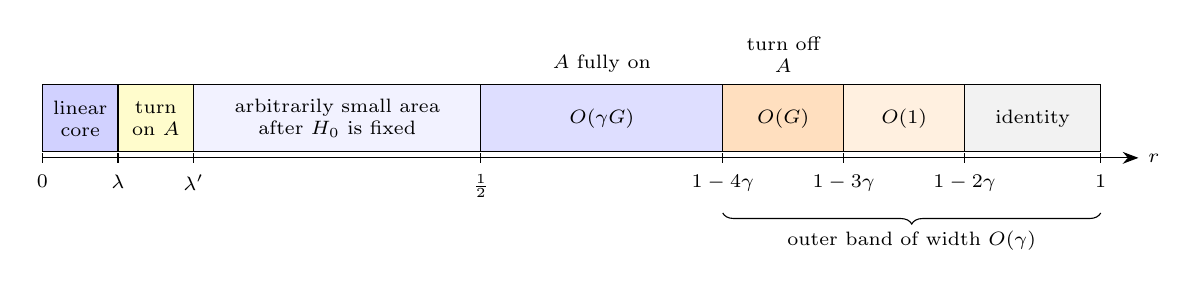
\begin{tikzpicture}[x=0.96cm,y=1cm,font=\scriptsize]
 \fill[blue!18] (0,0) rectangle (1,0.85);
 \fill[yellow!20] (1,0) rectangle (2,0.85);
 \fill[blue!5] (2,0) rectangle (5.8,0.85);
 \fill[blue!13] (5.8,0) rectangle (9,0.85);
 \fill[orange!25] (9,0) rectangle (10.6,0.85);
 \fill[orange!12] (10.6,0) rectangle (12.2,0.85);
 \fill[gray!10] (12.2,0) rectangle (14,0.85);
 \draw (0,0) rectangle (14,0.85);
 \foreach \x in {1,2,5.8,9,10.6,12.2} {\draw (\x,0)--(\x,0.85);}
 \node[align=center] at (0.5,0.42) {linear\\core};
 \node[align=center] at (1.5,0.42) {turn\\on $A$};
 \node[align=center] at (3.9,0.42) {arbitrarily small area\\after $H_0$ is fixed};
 \node at (7.4,0.42) {$O(\gamma G)$};
 \node at (9.8,0.42) {$O(G)$};
 \node at (11.4,0.42) {$O(1)$};
 \node at (13.1,0.42) {identity};
 \node[above] at (7.4,0.88) {$A$ fully on};
 \node[above,align=center] at (9.8,0.88) {turn off\\$A$};
 \draw[-{Stealth[length=2mm]}] (0,-0.08)--(14.5,-0.08)
       node[right] {$r$};
 \foreach \x/\s in {0/0,1/\lambda,2/\lambda',5.8/\tfrac12,
                     9/1-4\gamma,10.6/1-3\gamma,12.2/1-2\gamma,14/1}
       {\draw (\x,-0.02)--(\x,-0.15);\node[below] at (\x,-0.17) {$\s$};}
 \draw[decorate,decoration={brace,mirror,amplitude=4pt}]
       (9,-0.78)--(14,-0.78);
 \node[below] at (11.5,-0.88) {outer band of width $O(\gamma)$};
\end{tikzpicture}
\caption{Critical radial area costs in the pre-expansion coordinate
$r$; intervals are not drawn to scale.  Here
$G=1+lh/\dist(\omega,u_j)$ has bounded angular mean.  The linear core
contains no uncontrolled connector face.  Inner costs can be
suppressed after $H_0$ is fixed.  Among the remaining terms, the middle
band carries the factor $\gamma$, and terms without this factor occur
only in the thin outer band.}
\label{la:radial-bands}
\end{figure}

The measured connector surfaces after source squeezing are truncated
wedges.  Between $\lambda$ and $\lambda'$ they are exactly radial
over tile edges and are unchanged by $A$; their cost is arbitrarily
small with the increase of $e$ on that interval.  Below $\lambda$
these surfaces are absent.  On $[\lambda',1/2]$, all relevant
surfaces have positive angular clearance from the selected rays.
After $H_0$ and $\lambda'$ are fixed, choosing $\kappa,t$ sufficiently
small suppresses \eqref{la:two-angular}, and choosing $e'$ sufficiently
small suppresses \eqref{la:mixed-angular}.  Only finiteness of the
fixed surface areas is used in this step.  More explicitly, work in
units $h=1$ and let
\[
 M_0=\int_{\lambda'\le r\le1-4\gamma}G(\omega)\,d\mu<\infty,
\]
where $\mu$ is the unexpanded $H_0$-area of the finitely many surfaces.
Choose $\kappa$ below the angular clearance of every measured
surface on $\lambda'\le r\le1-\gamma$, including the switch-off
band.  This clearance follows from the inverse-ray sector condition
and compactness after removal of the exact germ.  Thus every use of
\eqref{la:angular-interpolation} on these surfaces lies in
$\rho\ge\kappa$.  The suppressed error is bounded by
\[
 C_b\left(\frac{t}{(\lambda')^2}
                +\frac{\alpha}{\lambda'}\right)M_0.
\]
The exact radial wedges on $[\lambda,\lambda']$ cost at most
$C_b L\alpha(\lambda'-\lambda)$, where $L$ is their total angular
edge length.  Thus $t$ and $\alpha$ can make the sum smaller than any
given positive error, while $k_\alpha$ remains positive and bounded
by $C\gamma$.

On the remaining fully-on band the mixed cost is at most
$C_b\gamma(1+lh/|\omega-u_j|)$ times unexpanded area; the
two-angular cost can again be suppressed.  On the switch-off band,
$l|\beta'|\le C l/\gamma=CK_0$, so
\eqref{la:angular-interpolation}--\eqref{la:mixed-angular} bound both
costs by a constant times the \emph{first} power of
$1+lh/|\omega-u_j|$.  The radial-only outer end has a fixed bounded
area factor.  Squaring the angular factor would not give the needed
averaging estimate, and is avoided by the determinant calculation.

\paragraph{A weight fixed before budgeting.}
Inside a retained volume block, the measured surface list consists
only of its full wedges.  Every other measured source surface lies
outside the block interior; kernel templates remain in their own
macro blocks.  The preimage of a selected target ray lies in the
open sector over its tile, so it meets neither these outside
surfaces nor a wedge, which lies on a sector boundary.  On compact
ray segments away from the exact germ, local finiteness therefore
gives positive clearance from the entire measured surface list.

In the outer radial region choose a continuous buffered majorant
$W$.  The angular envelope on a tile is a buffered version of
\[
 1+\frac{lh}{|\omega-u_j|}.
\]
Its singularity can be capped in a tiny neighborhood of the ray:
the ray-preimage sector condition makes the outer compact portions
of all measured surfaces disjoint from that ray.  First choose the
caps for the adjusted topological map with a positive margin, then
choose the budget mesh and $G,T$ fine enough to preserve the margin.
Cutoffs in disks of radius $O(lh)$ and a constant background make
the envelope continuous across tile boundaries.  Write the resulting
bounded envelope as $\widehat G$.  It agrees with an upper bound for
the uncapped factor on the measured surfaces and is bounded above
by a fixed multiple of the uncapped integrable envelope everywhere.

Choose continuous radial cutoffs with the following values, using
linear interpolation between the listed bands:
\[
\begin{array}{c|cc}
 &0&1\\ \hline
 \chi_{\mathrm{low}}&r\le1/2-\gamma&r\ge1/2\\
 \chi_{\mathrm{out}}&r\le1-6\gamma&r\ge1-5\gamma\\
 \chi_{\mathrm{cut}}&r\ge1-\gamma&r\le1-2\gamma.
\end{array}
\]
For a sufficiently large fixed $C_b$, take
\begin{equation}\label{la:outer-weight}
 W=\chi_{\mathrm{out}}+
   C_b\chi_{\mathrm{low}}\chi_{\mathrm{cut}}
             (\gamma+\chi_{\mathrm{out}})\widehat G.
\end{equation}
It is zero for $r\le1/2-\gamma$, dominates the required
$C_b\gamma G$ on the middle band and $C_bG$ on the return ramp,
and equals the ordinary weight one for $r\ge1-\gamma$.
The radial outer end is covered as well, and the angular factors
are confined below $1-\gamma$.  The part without the factor $\gamma$ occupies an
$O(\gamma)$ radial band.  Buffered cutoffs may enlarge these bands
by another fixed multiple of $\gamma$ without changing the estimates.

This fixes a bounded continuous weight before
Proposition~\ref{lt:budget-transfer} is applied.  The weight vanishes in
the star-modification neighborhoods, and the simplex map is the
identity on smaller exact-germ neighborhoods.  Thus the measured
crossings used by the transfer are the original $f$-crossings.  The
mesh-element suprema of $W$ give the weighted $H_0$-area upper bound.
The still smaller attenuation parameters in the preceding paragraph
are chosen \emph{after} $H_0$; they need not have been known when $W$
was fixed.  Equations~\eqref{la:two-angular} and
\eqref{la:mixed-angular} prove the asserted weighted bound for all
connector, outer, or nonincident measured surfaces, with arbitrarily
small additive errors.

\paragraph{Spokes and the final contractions.}
After the expansion, each shell spoke lies in a ball of radius
$C\gamma h$ about its intended outer mesh vertex.  Its entire image is outside the open linear $\lambda$-core by
injectivity and the exact germ, with the inner endpoint on that
core's boundary.  Its angular direction remains in a sufficiently
narrow vertex cone, and along the whole trace its pre-expansion
radius is at most $1+o(\gamma)$.  The angular maps fix vertices and have uniform local
Lipschitz bounds near them.  These facts give the stated ball
inclusion.

Each such spoke has finite length.  Homothetically contract its
entire vertex ball to a sufficiently tiny concentric ball, and extend
radially to the identity on the twice-larger ball.  The extension has
a uniform upper Lipschitz bound, while the homothety factor may be as
small as required to reduce the whole spoke length to
$C_b\gamma h$.  Group all spokes at a shared vertex and use the same
contraction for them.  The twice-larger balls are pairwise disjoint
when $K_0$ is large enough.  Their centers are outside the open cores.
There are $O(l^{1-m})$ boundary vertices, so their intersection with
a core has measure at most
\[
 C l^{1-m}(\gamma h)^m\le C\gamma h^m.
\]
On the core the map before contraction is $b$; hence the contracted
map still has derivative bounded by $C_b$.  All other length and
area estimates are multiplied by a bounded factor.  No uniform
inverse Lipschitz bound in the contraction factor is required.

\paragraph{Averaging the wedge weight.}
The total area of the full wedges in a three-dimensional block is
$O(h^2/l)$.  On their portions in $K$, $F=\Id$.  The outer band has
relative radial thickness $O(\gamma)$, and the remaining nonzero
weight has the factor $\gamma$.  Also, for a point $\omega$ fixed
before the choice of $u_j$,
\[
 \mathbb E_{u_j}\left[1+\frac{lh}{|\omega-u_j|}\right]\le C,
\]
because $u_j$ is sampled in two dimensions at scale $lh$.  An
indicator of successful selection can be dropped in this upper
bound.  Multiplying the resulting weighted area by $lh$ gives
$C_b\gamma h^3$ per block.

On off-$K$ wedge portions, use the same uncapped angular envelope
before making any clearance-dependent choices.  For normalized wedge
parameters $v$, translation continuity gives
\[
 \int_K
  \bigl(|Df|^2\mathbf1_{\Omega\setminus K}\bigr)(a+hv)\,da
       \longrightarrow0,
\]
and integration in the relative variables and wedge parameters
gives the corresponding averaged trace estimate.  The generic
surface formula in Lemma~\ref{lt:trace-slicing} applies.  This proves
\eqref{la:wedge-cost}, including the later target-mesh averaging of
Lemma~\ref{lt:budget-expectation}.  The outer grid has only
$O(l^{1-m})$ edges or faces at scale $lh$ per macro boundary, so its
converted bounded-derivative cost is $O_b(l)|Q|$.  Its off-$K$ error
tends to zero by the same trace averaging.  Nonincident edges avoid
the expansion; nonincident surfaces use the same clearance and
weighted estimate.  All required assertions follow.
\end{proof}

\subsection{Compact jets and kernel blocks}

We next reduce the remaining positive-rank sets to line and plane
sections.  The distinction between invertible, zero, and nonzero
singular derivatives already plays a central role in the planar
construction of Hencl--Pratelli
\cite[Section~1.1 and Section~3]{HenclPratelli2018}.  Here the singular
models are handled by compressing their kernel directions.  A matrix
with a prescribed rank need not be the derivative of any ambient
diffeomorphism; its kernel is used only to choose the source coordinates.

\begin{lemma}[Finite compact jet selection]\label{la:jet-selection}
Given $\varepsilon_0>0$, one can choose $M<\infty$ and finitely many
pairwise disjoint compact sets $K_i\Subset\Omega$, of ranks
$k_i\in\{1,2,3\}$, such that
\begin{equation}\label{la:jet-tail}
 \int_{\Omega\setminus\bigcup_iK_i}|Df|^p<\varepsilon_0.
\end{equation}
On their nonzero singular values there are common bounds $M^{-1}$
and $M$.  At rank three the sets have ambient $C^1$ diffeomorphism
charts $b_i$ agreeing with the values and derivatives of $f$, with
chart bounds $C_M$.  At ranks one and two, for any subsequently chosen
$\delta>0$, the pieces can be refined so that
\begin{equation}\label{la:rank-model}
 |Df-D_i|\le\delta\quad\hbox{on }K_i,
 \qquad \rank D_i=k_i,
\end{equation}
with the same type of singular-value bounds.  The compact pieces can
be enclosed in disjoint source neighborhoods and corresponding
disjoint target neighborhoods with buffers.  Once all finite
multiplicative constants are fixed, the neighborhoods can be chosen
so that
\begin{equation}\label{la:excess-neighborhood}
 \sum_i\int_{U_i\setminus K_i}(1+|Df|^p)
\end{equation}
is as small as prescribed, and the inverse images of the buffered
target neighborhoods lie in the corresponding $U_i$.
\end{lemma}

\begin{proof}
Sobolev maps are approximately differentiable almost everywhere.
Truncate the positive-rank sets where their nonzero singular values
lie in $[M^{-1},M]$, and choose $M$ so large that the lost derivative
integral is small.  Rank-zero points have zero derivative energy and
need not be included.  On each retained part, pass to compact subsets
with continuous jet data and uniform approximate differentiability,
losing an arbitrarily small further derivative integral.

These are $C^1$ Whitney jets after a further compact refinement.  To
see the value condition, take two nearby retained points and compare
their approximate first-order expansions at a common good point in
the overlap of balls of radius comparable to their separation.  The
uniform density losses can be made smaller than a fixed fraction of
the overlap, so such a point exists.  Subtracting the two expansions,
using continuity of the jets, and then sending the differentiation
error to zero gives the Whitney remainder estimate.  The $C^1$
extension theorem~\cite[Part~I, Section~4, Theorem~I]{Whitney1934} supplies the extensions.  At full rank, continuity
of the derivative and the inverse function theorem give local
invertibility.  Injectivity on the compact set, together with
compactness, makes the extension injective on a sufficiently small
neighborhood of the whole compact piece.  Its derivative and inverse
derivative bounds can be kept within $C_M$.

For ranks one and two, cover the bounded rank-$k$ matrix range by
finitely many $\delta$-balls centered at rank-$k$ matrices with
comparable nonzero singular values.  Refine the compact pieces
accordingly, losing an arbitrarily small integral to make the finite
pieces disjoint.  Their number does not enter the local chart
bounds.  Injectivity of $f$ makes their compact images disjoint as
well.  Regularity of the integrable measure $(1+|Df|^p)\,dx$ gives
\eqref{la:excess-neighborhood}; continuity of $f^{-1}$ permits target
buffers whose preimages stay inside these source neighborhoods.
The initial losses can be allocated to give
\eqref{la:jet-tail}.
\end{proof}

Use Lemma~\ref{lt:source-mesh} with mesh sizes at most $lh$, deep
cubical regions around the $K_i$, and a common macro shift within
each such region.  At rank $k=1,2$, choose orthonormal coordinates
$x=(y,z)$ with $z\in\ker D_i$ and $y\in\R^k$.  At rank three use
Lemma~\ref{la:radial-blocks}.  A failed macro block is left as ordinary
fine cells.  Outside the retained macro blocks all cells are ordinary,
including the locally finite cells approaching $\partial\Omega$.

The anisotropic target grids of Lemma~\ref{lt:sharp-grid} are needed
only at rank one and at rank two when $p=2$.  Their long directions
span $\operatorname{range}D_i$, their aspect parameter is $\eta>0$,
and a linear normalization $L_i$ can be chosen so that
\begin{equation}\label{la:normalization}
 L_iD_i(y,z)=(y,0),\qquad
 \|L_i\|+\|L_i^{-1}\|\le C_M.
\end{equation}
The range and its orthogonal complement remain orthogonal in this
normalization.  Elsewhere the target grid can be isotropic.

Consider one rank-$k$ candidate macro cube $Q$ of side $h$.  Let $B$
be its concentric product cube obtained by removing one fine layer
from each side, let $Y$ be its projection onto the $y$-coordinates,
and let $z_0$ be its central kernel coordinate.  Put
\[
 S=Y\times\{z_0\}.
\]
Construct a Lipschitz map
\begin{equation}\label{la:flat-collapse}
 P_0(y,z)=(y,p_y(z)):Q\longrightarrow Q
\end{equation}
which is the identity on $\partial Q$ and collapses $B$ onto $S$.
For $y\in Y$, collapse the inner kernel cube to $z_0$ and extend
radially and linearly to the outer kernel boundary.  Outside $Y$,
blend with the identity using a piecewise smooth $y$-cutoff.  These
formulas may be chosen semialgebraic and piecewise $C^1$ on closed
pieces, with Lipschitz bound $C_l$.  They preserve $y$ exactly, so
\begin{equation}\label{la:collapse-model-identity}
 D_iDP_0=D_i.
\end{equation}
For $0<\lambda\le1$, put
\begin{equation}\label{la:positive-collapse}
 P_\lambda=(1-\lambda)P_0+\lambda\Id.
\end{equation}
For each fixed $y$ the kernel radial slopes are positive.  The map is
triangular in $(y,z)$, fixes the boundary, and is bi-Lipschitz on $Q$.

Budget the shell edges after $P_0$, and also its shell faces when
$p=2$.  Include $S$, its tile edges, and all lower-dimensional
intersections that occur in these templates.  In source and target
units divided by $h$, require that the sum of the $p$-power
tangential derivative errors from the model on these finitely many
pieces is at most $\tau^p$.  On a $P_0$-image this means the error
from $D_iDP_0=D_i$; on $S$ it means the error from its $y$-columns.
The unprojected section is required to carry its Sobolev trace even
when $k=2,p<2$.

\begin{lemma}[Successful kernel blocks]\label{la:kernel-selection}
For fixed $M,l,\tau$, the total expected volume of candidate
rank-one or rank-two blocks failing these trace tests tends to zero
as first $\delta\to0$ and then $h\to0$, with sufficiently small
excess neighborhoods.  In successful blocks the transferred
unparametrized shell data have converted cost
\begin{equation}\label{la:kernel-shell-budget}
 O_M(l)\sum_Q|Q|+\text{an arbitrarily small error}.
\end{equation}
Here converted edge cost means $(lh)^{3-p}$ times image length to the
power $p$, and, when $p=2$, converted face cost means $lh$ times
image area.  Fixed factors depending on $l$ and $\eta$ are allowed
on the trace errors.
\end{lemma}

\begin{proof}
Translation averaging on the fixed product templates, with block
weight $h^3$, bounds the expected sum of normalized trace errors by
\begin{equation}\label{la:trace-test-expectation}
 C_l\sum_i\int_{N_{Ch}(K_i)}|Df-D_i|^p.
\end{equation}
The measured curve strata, and the measured surface strata when $p=2$,
are covered by Lemma~\ref{lt:trace-slicing}. For the additional
unprojected rank-two plane section when $p<2$, ordinary Sobolev slicing
and translation Fubini supply the $W^{1,p}$ trace used in these tests.
This step requires neither an image-area formula nor a two-dimensional
Lusin property. On $K_i$, the integrand is at most
$\delta^p$; off $K_i$ it is bounded by
$C_M(1+|Df|^p)$, whose excess integral is small.  Markov's inequality
therefore makes the failed volume small relative to the fixed
threshold $\tau^p$.

There are $O(l^{-2})$ shell cells of side $lh$.  In grid units, with
the longest side restored after the anisotropic rescaling,
\eqref{la:collapse-model-identity} prevents inflation of the model
term.  The factors from $DP_0$ and from anisotropy multiply only
$Df-D_i$.  Lemma~\ref{lt:curve-probability}, followed by H\"older
on each curve, gives the edge length-power budgets.  At $p=2$,
Lemma~\ref{lt:budget-expectation} and the squared derivative trace
integrals give the face budgets.  A bounded model derivative costs
$C_M(lh)^3$ per shell cell after conversion; multiplying by
$O(l^{-2})$ gives $C_Mlh^3$ per macro block.  For fixed $l,\eta$, the
error contributions are made as small as desired by $\tau$ and the
budget-transfer tolerances.  All relevant images lie deep inside
their prescribed target patches for small $h$, by the source and
target buffers.  This proves \eqref{la:kernel-shell-budget}.
\end{proof}

\subsection{Parametrizing the retained line and plane sections}

For a successful rank-$k$ block we shall find a bi-Lipschitz
self-homeomorphism $\sigma_Y$ of $Y$, preserving its tile complex,
and a tangential map $h_Y$ into the target.  If $V$ denotes the initial
map $H_0$ after all the required output motions, the relation is
\begin{equation}\label{la:section-parametrization}
 h_Y(y)=V(\sigma_Y(y),z_0).
\end{equation}
The aim is
\begin{equation}\label{la:section-goal}
 \sum_{\text{successful }Q}
   h^{3-k}\int_Y |Dh_Y-D_i|_y^p
       \quad\hbox{arbitrarily small}.
\end{equation}
Only the $y$-columns of $D_i$ occur in this formula.  The factor
$h^{3-k}$ is the volume of the kernel fibers, up to fixed constants.

\paragraph{Rank one.}
On each interval tile, reparametrize the transferred curve at
constant speed in the normalization $L_i$.  By
Lemma~\ref{lt:sharp-grid}, its expected length budget, divided by
the tile length, is at most
\begin{equation}\label{la:sharp-length-budget}
 1+C_M\eta+o_{\tau}(1)+o_{\mathrm{transfer}}(1),
\end{equation}
where $l$ and $\eta$ have already been fixed.  Its budget is also at
least $1-o(1)$: the section trace test gives almost correct endpoint
differences, and a sufficiently fine transfer preserves the values
to a still smaller error.  Consequently the total positive excess,
weighted by tile length times $h^2$, has arbitrarily small expectation.

The constant speeds are bounded by $C_M$ simultaneously, using
Lemma~\ref{lt:curve-probability}.  To see that its grid-unit constants
do not deteriorate with $\eta$, split the normalized trace derivative
into the tangent model and the error.  The model has size bounded by
$C_M$ in longest-side-restored grid units.  The error has $p$-mean at
most $C_{\eta,l}\tau$, and is made small after the grid parameters
are fixed.

Here is the elementary sharpness calculation.  On a unit normalized
interval, write $u$ for the constant-speed curve, $s=|u'|$, and
$d=u(1)-u(0)$.  If $e$ is the desired unit direction, then
\begin{equation}\label{la:length-sharpness}
 \int_0^1|u'-e|^2=s^2+1-2e\cdot d.
\end{equation}
Since $s\le C_M$, $|d-e|$ is small, and $s\ge1-o(1)$, the right side
is bounded by $C_M(s-1)_+$ plus an arbitrarily small error.
For $1\le p\le2$, H\"older converts this squared error to a
$p$-error.  Rescaling the tiles and summing with the fiber weights
proves \eqref{la:section-goal}.  In particular the argument works at
$p=1$; it does not appeal to strict convexity of the $L^1$ norm.

\paragraph{Rank two at the critical exponent.}
Now $k=p=2$.  For every planar tile, use the area budget in the
normalization $L_i$.  Lemma~\ref{lt:sharp-grid}, applied to its
oriented tangent $2$-vector and the squared derivative trace error,
gives expected normalized area at most
\begin{equation}\label{la:sharp-area-budget}
 1+C_M\eta+o_\tau(1)+o_{\mathrm{transfer}}(1).
\end{equation}
There is also the lower bound $1-o(1)$ for every sufficiently fine
generic sample.  Indeed the edge tests make the original boundary
trace uniformly close, after translation and normalization, to the
boundary of the identity square.  The transfer preserves that
closeness.  Orthogonal projection of the transferred disk to the
model plane has degree one at every point a small distance inside
the square.  It therefore covers that inner square, and its area is
at least the inner-square area.  Since the transferred area is no
larger than its budget plus a chosen small error, the same lower
bound holds for the budget.  These tiles lie away from all exempt
star centers.

It follows that the weighted sum of the positive area excesses has
arbitrarily small expectation.  To obtain the needed boundary
parametrization, subdivide each common edge into $J$ fixed intervals
and use constant speed on each interval, preserving its endpoints.
Choose $J$ large before the finer trace and transfer tolerances.
Lemma~\ref{lt:curve-probability} bounds the normalized speeds by
$C_M$; the error part is $C_{\eta,l,J}\tau$ and is made small later.
Every reparametrized point stays within its $J$-interval, so the
boundary values converge uniformly to the ideal translated square
as $J\to\infty$ and the finer errors tend to zero.  The boundary
squared derivative integral is uniformly bounded.

Absorb these common edge changes by coning in each tile, then apply
Lemma~\ref{lt:disk}.  Fix a desired derivative tolerance $\zeta>0$.
The sharp assertion of Lemma~\ref{lt:disk} supplies an area-excess tolerance
$\rho>0$ and a boundary-closeness tolerance, using the already fixed
speed bound.  On tiles whose normalized area is at most $1+\rho$,
it gives squared derivative error at most $\zeta$ in tile units.
For the remaining tiles, the sum of their converted tile measures
is bounded by $\rho^{-1}$ times the positive excess.  The crude disk
estimate bounds their energy by a constant times area plus the
bounded boundary energy.  Thus their total converted energy is at
most
\[
 C_M(1+\rho^{-1})\,
       \bigl(\hbox{total converted positive excess}\bigr)
       +o(1).
\]
Make the positive excess small after fixing $\rho$.  This proves
\eqref{la:section-goal} also in the critical rank-two case.  The
finite-piece and edge regularity needed by the disk estimate will
be checked below before the volume gluing.

\paragraph{Rank two below the critical exponent.}
Suppose $k=2$ and $1\le p<2$.  The macro selection has already fixed
finitely many plane sections.  On each $S$, first discard points
where the tangential derivative differs substantially from the
injective $y$-columns of $D_i$.  On the retained set its two singular
values lie between bounds depending only on $M$.  The trace test and
Chebyshev's inequality show that the discarded integral of
$1+|D_yf|^p$ is at most $C_M\tau^p h^2$.  Select compact $C^1$ Lusin
jet sets in the interiors of the original tiles, losing an
arbitrarily small additional integral.  The jets extend to ambient
charts $b$ by adding a normal column with the ambient orientation of
$f$.  Their derivative and inverse derivative bounds are $C_M$.
Thus the leftover part of the section satisfies
\begin{equation}\label{la:section-leftover}
 h^{-2}\int_{\text{leftover}}(1+|D_yf|^p)
       \le C_M\tau^p+\text{an arbitrarily small error}.
\end{equation}
Choose disjoint compact neighborhoods on the source and target sides.
The new compacts avoid the original tile edges.  They also avoid
$P_0$ of every shell edge: when those images lie in $S$, their
$y$-coordinates belong to the tile boundaries.  Consequently all
these fixed graph images have positive clearance from the new
compact neighborhoods.

Inside each section use a new macro grid of side $s$ and a fine grid
of side $ls$, with $s\to0$ only after the macro data have been fixed.
To respect the original tile seams, insert their fixed coordinate
levels, omit shifted $s$-levels within $s/4$ of a seam, and subdivide
each remaining gap into $N$ equal pieces.  The resulting rectangles
have controlled aspect ratios.  Near a seam, every nonfixed
subdivision level has a shift coefficient of magnitude at least
$1/N$, so its translation density is bounded for fixed $l$.
Only boundedly many such levels occur per seam in an $O(s)$ band.
Therefore their edge trace integrals, multiplied by $ls$, are bounded
in expectation by $C_l$ times the section derivative integral on
that shrinking band.  The fixed seam lines have finite trace
integrals and their converted weights tend to zero.  Both
contributions vanish as $s\to0$.

Apply Lemma~\ref{la:radial-blocks} with $m=2$ on the new compacts,
simultaneously with the preparation of $H_0$.  All target radial and
vertex motions avoid the already-budgeted fixed graph because of the
clearance just established.  On each successful micro block, make
the radial source change only as a parametrization of the section,
and keep its controlled core.  Parametrize the remaining planar
edges at constant speed, except for the prescribed core edges, and
apply Lemma~\ref{lt:collapse} to the remaining two-dimensional cells.
It applies because $p<2$.  Do the same on fallback micro cells.
These changes fit together to form a tile-preserving bi-Lipschitz
map $\sigma_Y$ of the section.  They are not inserted as an
additional ambient precomposition.

On the compact jets in the micro cores, the map equals $b$, apart
from the bounded-derivative caps of Lemma~\ref{la:radial-blocks}; its
derivative is $D_yf$ there.  The cap fraction and shell contributions
are $O_M(l)$ in section units.  The derivative is bounded by $C_M$
on the remaining core portions.  The shell spokes have image length
$O_M(\gamma s)$, so constant-speed parametrization gives their
required bounded energy.  Ordinary outer and fallback edges use the
individual high-probability length bounds, followed by the planar
collapse estimate.  The latter has the form
\[
 \int_D|Dg|^p
       \le C(ls)\int_{\partial D}|D_tg|^p+\text{a chosen error}.
\]
Translation averaging and \eqref{la:section-leftover} therefore give
\begin{equation}\label{la:micro-section-error}
 h^{-2}\int_Y|Dh_Y-D_i|_y^p
       \le C_M l+C_M\tau^p+o_s(1)
                 +\text{an arbitrarily small error}.
\end{equation}
Here failed micro blocks contribute vanishing cost by their failed
area and bounded compact jets; elsewhere the ordinary converted
trace cost is bounded by the leftover integral.  The constants in
that latter bound depend on $M$, not on later micro-chart widths or
their number.  The seam errors were handled separately above.
Multiplying by $h$ and summing proves \eqref{la:section-goal}.
On the original tile edges, the same construction gives an upper
$p$-energy bound by a fixed constant times the original trace
$p$-energy plus chosen errors.  There are no micro output motions
on those edges.

\subsection{From section cores to volume cells}

We now keep all finite section data and output motions fixed.  On a
rank-$k$ macro core use
\begin{equation}\label{la:kernel-core-map}
 G_\lambda(y,z)
   =V\bigl(P_\lambda(\sigma_Y(y),z)\bigr),\qquad(y,z)\in B.
\end{equation}
Since $P_0$ is flat on $B$, its argument here is
\[
 (\sigma_Y(y),z_0+\lambda(z-z_0)).
\]
Lemma~\ref{la:composition-limit} gives
\begin{equation}\label{la:kernel-core-limit}
 DG_\lambda\longrightarrow[Dh_Y,0]
       \quad\hbox{in }L^p(B)\qquad(\lambda\downarrow0).
\end{equation}
The outer map $V$ has finitely many closed-piece $C^1$ formulas on
the compact configurations: this is true for $H_0$ and for each
radial, angular, and cap map.  The inner maps are uniformly Lipschitz
for fixed $\sigma_Y$, and their derivatives have the stated pointwise
limit.  This verifies the hypotheses even if the limiting map has
rank one or two.

The core boundary values preserve the images of its individual facets.
Indeed, set
\[
 w_\lambda=V\circ P_\lambda,\qquad
 T_B(y,z)=(\sigma_Y(y),z).
\]
Then $G_\lambda=w_\lambda\circ T_B$ on $B$.  Since $\sigma_Y$ preserves
the tile complex, $T_B$ preserves each fine facet and edge of
$\partial B$.  In particular,
\[
 G_\lambda(F)=w_\lambda(F)
 \quad\hbox{for every such facet }F.
\]
Thus these boundary values can be prescribed on the adjacent shell
cells without changing their base face images.  The product formula
need not be extended through the shell; its base map there is
$w_\lambda=V\circ P_\lambda$.
Apply Lemma~\ref{la:composition-limit} separately on its edges and
faces, with limiting parameter map $P_0$.  Their lengths and areas
converge to the transferred budgets, or to smaller upper bounds
when rank is lost.

We record the boundary scaling of the prescribed core data.  Facets
normal to a kernel coordinate have limiting energy bounded by
\begin{equation}\label{la:normal-kernel-face}
 C h^{2-k}\int_Y|Dh_Y|^p.
\end{equation}
For $k=2$, facets normal to a $y$-coordinate use the original tile-edge
parametrizations on $\partial Y$; their total energy per macro block
is $O_M(h^2)$.  For $k=1$ their limiting energy is zero.  The total
limiting edge energy on the subdivided $\partial B$ is
\begin{equation}\label{la:core-edge-energy}
 O_M(h/l).
\end{equation}
For the critical rank-two case this follows from the uniform edge
speed bounds.  Below the critical exponent use instead the
individual original tile-edge energy estimates just proved; the
trace tests bound their sum.  Edges replicated in kernel directions
have the same tangential data, and kernel-axis edges have zero
limiting energy.  Multiplying \eqref{la:normal-kernel-face} by $lh$
and \eqref{la:core-edge-energy} by $(lh)^2$ gives
$O_M(l)$ times the macro-volume contributions, using
\eqref{la:section-goal} for the first expression.  Small positive
$\lambda$ preserves these estimates with arbitrarily small error.

\begin{lemma}[Completion of uncontrolled cells]\label{la:cell-completion}
Let $D$ be an uncontrolled source three-cell of scale $H$ in the
construction.  Its base embedding $v:D\to\R^3$ is bi-Lipschitz and is
given by finitely many $C^1$ formulas extending to neighborhoods of
their closed pieces.  Write $g$ for the prescribed or subsequently
chosen boundary data.  On every prescribed core face $F$,
assume that $g|_F=v|_F\circ s_F$, where $s_F:F\to F$ is a
bi-Lipschitz self-homeomorphism preserving each edge.  These self-maps
agree on shared edges.  When $p=2$, their edge restrictions have
derivatives with essential limits almost everywhere.
Then the cell can be reparametrized bi-Lipschitzly, preserving its
base image and all prescribed boundary data, with derivative cost
at most a constant times
\begin{equation}\label{la:cell-cost}
 \begin{split}
 H\sum_{F\text{ prescribed}}\int_F|D_tg|^p
 &+H^2\sum_{e\subset\partial D}\int_e|D_tg|^p\\
 &+\mathbf1_{\{p=2\}}\,
       H\sum_{F\text{ uncontrolled}}\operatorname{Area}(v|_F)
 \end{split}
\end{equation}
plus any prescribed positive error.  An unprescribed edge of length
comparable to $H$ may be given energy at most
$C\operatorname{length}(v(e))^pH^{1-p}$.
The constants depend only on $p$ and the fixed shape bounds, and
adjacent cells can be completed with identical shared-face data.
\end{lemma}

\begin{proof}
First reparametrize every unprescribed edge at constant speed,
keeping common vertices.  On an unprescribed face, cone-extend these
edge changes.  If $p<2$, Lemma~\ref{lt:collapse} in dimension two gives
face energy bounded by $CH$ times its boundary $p$-energy plus a
chosen error.  If $p=2$, use the crude estimate of
Lemma~\ref{lt:disk}; after scaling it bounds the face energy by a
constant times its base image area plus $H$ times its edge squared
energy.  Shape-controlled polygons are converted to square
parameters by fixed bi-Lipschitz closed-piece smooth charts.
Prescribed faces are left with their given parametrizations.  Make
one choice per shared face.

The disk hypotheses follow from the actual base and edge regularity.
Restricting finitely many closed-piece $C^1$ formulas gives the
almost-everywhere essential limits on a base face and the tangential
limits at its parameter edges.  On each fixed edge subdivision,
normalized arclength has derivative with essential limits almost
everywhere.  Bi-Lipschitzness bounds that derivative away from zero,
and the inverse arclength map has the same property.

For prescribed kernel edges, the source self-map is the restriction
of $T_B$.  In the rank-one case it is the interval arclength change;
in the critical rank-two case it is the arclength change on each fixed
$J$-subinterval of the section edge.  The disk parametrizations fix the
tile boundaries, so they leave these edge changes intact.  Kernel-axis
edges use the identity.  Reusing these source self-maps at positive
$\lambda$ retains their essential derivative limits, even though the
resulting curves need not have constant speed for the base map
$w_\lambda$.  On radial-core facets the prescribed map already equals
$v$, so $s_F=\Id$.  Thus all prescribed edges needed for a critical
face satisfy the stated condition.  Coning the edge changes preserves the
compatibility required by Lemma~\ref{lt:disk}.

The assembled boundary map $g$ gives the face-preserving bi-Lipschitz
self-homeomorphism $v^{-1}\circ g$ of $\partial D$.  Apply
Lemma~\ref{lt:collapse} to this boundary self-map in dimension three,
where $p\le2<3$.
It contributes a factor $H$ times the true boundary-face energy.
Substituting the preceding face estimates gives
\eqref{la:cell-cost}.  This last collapse requires the radial
compatibility of the base parametrization and a fixed bi-Lipschitz
boundary map; it does not require stronger smoothness of the entire
boundary reparametrization.  Allocate the intermediate errors so
their converted sum is below the prescribed cell error.
\end{proof}

\subsection{Global choices, summability, and strong convergence}

\begin{proof}[Proof of Theorem~\ref{la:approximation}]
We first construct locally bi-Lipschitz approximants; smoothing is
performed only after their global derivative costs have been
estimated.  If necessary, compose with a reflection to fix an
orientation convention, and undo it at the end.

\paragraph{Order of the fixed data.}
Let $\varepsilon_0>0$ be a tail tolerance, to be sent to zero.
Choose the compact rank truncation and its bound $M$ in
Lemma~\ref{la:jet-selection}.  Choose $l$ so small that all the
$O_M(l)$ contributions in volume and section shells and in cap
regions are below a prescribed auxiliary tolerance.  Recall that
$\gamma=l/K_0$.

With $M,l$ fixed, choose the sharp derivative tolerances for the
line and plane tiles.  The speed bounds entering those tolerances
are fixed in terms of $M$.  When $k=p=2$, choose the further edge
subdivision $J$ large enough for the desired boundary closeness.
Choose $\eta$ small enough for the sharp length and area coefficients,
then $\tau$ small enough for all trace errors, including the factors
depending on $l,\eta,J$.  Next choose $\delta$ in
\eqref{la:rank-model} small enough, refine the compact pieces, and
choose their nested excess neighborhoods so that
\eqref{la:excess-neighborhood} is small after multiplication by every
now fixed inflation factor.  These bounds do not depend on the
widths of the neighborhoods or on the number of their compact
pieces.  Only then choose $h$ small and make the macro success
selections.  The planar micro configurations, when present, are
chosen afterward, using \eqref{la:section-leftover} and then small
$s$.  Their ambient chart constants are controlled by $M$.

Fix the bounded radial area weights and compact clearance margins
before choosing the target budget mesh.  Choose that mesh using
Proposition~\ref{lt:budget-transfer} and Lemmas~\ref{lt:budget-expectation},
\ref{lt:curve-probability}, and~\ref{lt:sharp-grid}.  This determines
$H_0$, with the required exact affine germs.  The small radial
parameters, angular attenuation parameters, and vertex contractions
are then chosen from the actual finite configuration.  In kernel
blocks choose $\lambda$ after the section parametrizations and all
output maps have been fixed.  Finally complete the uncontrolled
cells using Lemma~\ref{la:cell-completion}, with summable positive
error prescriptions.  Lemma~\ref{pre:local-tolerances} permits the
locally finite fine choices and these summable prescriptions.

\paragraph{Controlling ordinary and failed cells.}
We give the accounting that makes this order of choices sufficient.
For ordinary cells meeting no compact jet set and no enlarged special
neighborhood, source sampling bounds the converted trace integrals in
expectation by
\begin{equation}\label{la:ordinary-tail}
 C_p\int_{\Omega\setminus\bigcup_iK_i}|Df|^p.
\end{equation}
On the simultaneous individual curve-bound event, H\"older's inequality
bounds the converted edge costs by these source trace integrals.  When
$p=2$, the conditional expectation over the later target mesh bounds
the converted face-area budgets by the corresponding source traces.
Substituting in \eqref{la:cell-cost} gives precisely the codimension
conversion factors $H$ for faces and $H^2$ for edges.  The constants in
\eqref{la:ordinary-tail} are ordinary mesh and budget constants,
independent of $M,l,\eta$.

In a failed macro block, the compact-jet integrands are bounded by a
constant depending on $M$.  For the ordinary fine grid, the total
converted size of edges and faces in that block is $O(h^3)$, with
fixed factors from any special target normalization allowed.
The converted source trace integrals over its compact-jet portions
are therefore bounded deterministically by $C h^3$.  After the source
mesh and failed blocks have been selected, the target area-budget
expectation applies to these fixed traces.  On the individual
curve-bound event, H\"older's inequality gives the same bound for
converted edge costs.  Thus the small failed-block volume controls
their total without requiring a source trace law conditional on
failure.  On off-compact portions, discard the failure indicator
before applying the unconditional source trace bounds.

Whenever a nonuniversal constant can occur, its whole source trace
lies in one of the chosen enlarged source neighborhoods for small
enough meshes.  Indeed its image meets a buffered anisotropic or
radial-motion zone, whose inverse image is compactly inside that
neighborhood; the small cell diameter and the fine initial-map
errors preserve this inclusion.  Thus even an edge length-power
estimate can pay its finite factor on the \emph{whole} edge's
H\"older integral, then split this integral into the bounded
compact-jet part and the small excess part.  By
\eqref{la:excess-neighborhood}, all these excess contributions are
as small as prescribed.  No later large constant multiplies the
unprotected tail in \eqref{la:ordinary-tail}.

For full-rank radial blocks, Lemma~\ref{la:radial-blocks} gives the
small wedge budget and the contracted spoke lengths.  On compact
points of a failed full-rank block, $F=\Id$, so their image points
cannot belong to another block's inset angular support.  Outer
ordinary traces of retained blocks have the $O_M(l)$ converted cost
already computed.  Any off-compact surface portion affected by an
angular map is estimated by the uncapped envelope, integrating in
$u_j$ before the later clearance-dependent caps.  Its conditional
mean is bounded for the fixed trace template.  This gives the same
small excess estimate.  Nonincident edges avoid the angular
supports and hence never pay a power of that angular envelope.
Target-mesh suprema of the fixed bounded weights are allowed an
arbitrarily small enlargement error by a still finer target mesh.

The kernel shells are controlled by
Lemma~\ref{la:kernel-selection},
\eqref{la:normal-kernel-face}, and
\eqref{la:core-edge-energy}.  Their prescribed face and edge
contributions in \eqref{la:cell-cost} are $O_M(l)$ in bulk units.
The radial volume shells have the same bound, since their prescribed
core faces have bounded derivatives and their radial edges have
length $O_M(\gamma h)$.  All estimates are relative to the original
straight product or frustum cell sizes; no shape bound is imposed
on the intermediary image cells.

\paragraph{Simultaneous choices.}
Each estimate just used bounds a sum of nonnegative errors.  In the
sharp line and plane cases, this sum is the positive excess, not the
signed total excess alone; the lower bounds in the section argument
are what allow that replacement.  Choose the expectations smaller
than the desired tolerances with enough slack, and use Markov's
inequality for the finitely many aggregate objectives.  The source
and micro configurations are fixed first, using the trace,
failed-volume, and angular-weight bounds.  The target sample is
chosen next, meeting the expectation objectives together with the
arbitrarily high-probability individual curve bounds.  Countably
many ordinary curves are handled with summable failure allowances
and local mesh upper bounds.  Generic slicing and intersection
conditions have full measure on their templates; the star conditions
have already been accounted for by the small failed volume.

In particular, the sharp disk tolerances are selected using fixed
speed bounds.  Make the positive excess small only after their area
threshold $\rho$ is chosen.  The converted measure of bad sharp
tiles and their crude energy are then small by the explicit
$\rho^{-1}$ estimate above.  This avoids any assertion that the
lattice intersection count itself converges pointwise on a
wrinkled trace.  These choices yield deterministic configurations
with all the stated bounds simultaneously.

\paragraph{The resulting homeomorphism.}
Let $V$ be $H_0$ after the ambient radial-angular expansions and the
vertex contractions.  Their supports are disjoint within each
family.  Distinct compact configurations have separated target
neighborhoods; the much later micro-section supports were chosen
smaller still, and avoid all fixed graph data.  In the rank-three
volume blocks precompose by the radial source squeezes.  In kernel
blocks use $P_\lambda$ as the shell base map and
\eqref{la:kernel-core-map} on the core.  Section micro squeezes enter
only through $\sigma_Y$.  Complete all remaining edges, shared faces,
and volume cells as in Lemma~\ref{la:cell-completion}.

Each change is a self-parametrization relative to the same base
image, with matching boundary values.  The meshes are locally finite,
and each interior compact meets only finitely many pieces.  Finite
local straight cell geometry and the finite local bi-Lipschitz
constants give a locally bi-Lipschitz map across the interfaces.
It is a homeomorphism of $\Omega$ onto the same target as $V$.
The initial $H_0$ is onto $\Omega'$, and every output change is a
self-homeomorphism supported inside $\Omega'$.  Consequently the
assembled map $H$ is onto exactly $\Omega'$.

\paragraph{Derivative error.}
Let $\mathcal C$ be the union of the controlled volume cores.  The
preceding bounds imply
\begin{equation}\label{la:outside-core-energy}
 \int_{\Omega\setminus\mathcal C}|DH|^p
       \le C_p\varepsilon_0+o(1),
\end{equation}
where the auxiliary errors, including $O_M(l)$, can be made as small
as prescribed in their stated order.  The original derivative has
the same small bound on this complement: outside the compacts use
\eqref{la:jet-tail}, while on the compacts the shell fraction and
failed volume are small and the jets are bounded.

On a full-rank core, $H=b_i$ except on the small bounded-derivative
caps.  On its compact jet set, $Db_i=Df$; on the remaining portion the
chart derivative is bounded and the excess integral is small.
Thus the derivative difference there is small.  On a kernel core,
\eqref{la:kernel-core-limit} and \eqref{la:section-goal} give closeness
to $D_i$ with the correct fiber factor $h^{3-k}$.  Equation
\eqref{la:rank-model} compares $D_i$ with $Df$ on $K_i$, and the
excess-neighborhood bound treats the remaining points.  Choose the
finitely many $\lambda$'s sufficiently small after the other data.
Combining these estimates with \eqref{la:outside-core-energy} yields
\begin{equation}\label{la:derivative-final}
 \int_\Omega|DH-Df|^p\le C_p\varepsilon_0+o(1).
\end{equation}
All uncontrolled-cell errors were chosen summably.  The displayed
bounds therefore also establish $\int_\Omega|DH|^p<\infty$, rather
than only local Sobolev regularity.

\paragraph{Value convergence.}
The source self-parametrizations move points only within cells or
blocks whose maximum diameter tends to zero.  The initial budget map
can have arbitrarily small value error, and the target motions are
supported in boxes of arbitrarily small diameter in physical
coordinates.  On every interior compact, continuity of $f$ then
gives value convergence.  Since the domains are bounded and all
images lie in the fixed bounded target, dominated convergence gives
$L^p$ convergence on $\Omega$.  Choose the meshes and value
prescriptions so its error and \eqref{la:derivative-final} sum to less
than the prescribed $\eps$; this proves \eqref{la:goal}.

\end{proof}

\section{Completion on the fixed target}\label{sec:completion}

\begin{proof}[Proof of Theorem~\ref{main:theorem}]
Fix $1\le p\le2$ and $\varepsilon>0$. Apply Theorem~\ref{la:approximation} with sufficiently small error, obtaining a locally bi-Lipschitz homeomorphism $H:\Omega\to\Lambda$ in $W^{1,p}$. Apply Theorem~\ref{sm:smoothing} to $H$ with a smaller error. The triangle inequality gives a smooth diffeomorphism $g:\Omega\to\Lambda$ such that
\[
 \int_\Omega (|g-f|^p+|Dg-Df|^p)\,dx<\varepsilon.
\]
Both approximation theorems give global $W^{1,p}$ membership and retain
the target for each approximant. In particular, the proper-degree
argument in Lemma~\ref{sm:proper-degree}, used during smoothing,
establishes bijectivity before any limit is taken; the nonsingular
smooth differential then supplies the smooth inverse. Apply the
construction with $\varepsilon=2^{-j}$ to obtain
\eqref{main:convergence}.
\end{proof}

\begingroup
\raggedright
\bibliographystyle{plainnat}
\bibliography{references}
\endgroup
\end{document}
